
\documentclass[11pt, a4paper]{book}
\usepackage{svn-multi}
\svnid{$Id$}
% \usepackage{prelim2e}
\newcommand{\PrelimWords}{Draft Copy \svnkw{Id}}
%%\newcommand*{\mysvnrev}{\svnrev}
\usepackage[hyperindex=true,
			bookmarks=true,
            pdftitle={}, pdfauthor={Xi Yang},
            colorlinks=false,
            pdfborder=0,
            pagebackref=false,
            citecolor=blue,
            plainpages=false,
            pdfpagelabels,
            pagebackref=true,
            hyperfootnotes=false]{hyperref}
\usepackage[all]{hypcap}
\usepackage[palatino]{anuthesis}
\usepackage{afterpage}
\usepackage{graphicx}
\usepackage{thesis}
\usepackage[square]{natbib}
\usepackage[normalem]{ulem}
\usepackage[table]{xcolor}
\usepackage{makeidx}
% \usepackage{cleveref}
% \usepackage[centerlast]{caption2}
\usepackage{float}
\urlstyle{sf}
\renewcommand{\sfdefault}{uop}
\usepackage[T1]{fontenc}
\usepackage[scaled]{beramono}

\usepackage{multirow}

% Thesis style guide:
% https://policies.anu.edu.au/ppl/document/ANUP_012815

\renewcommand*{\backref}[1]{}
\renewcommand*{\backrefalt}[4]{
  \ifcase #1 %
    %
  \or
    (cited on page #2)%
  \else
    (cited on pages #2)%
  \fi
}



%!tex root=./thesis.tex
%      $Id: macros.tex 506 2009-10-05 16:57:07Z daniel $    

\usepackage{booktabs}
\usepackage{relsize}
\usepackage{xspace}

\definecolor{tableheadcolor}{rgb}{0.8,0.8,1.0}
%\definecolor{tablealtcolor}{rgb}{0.9,0.9,1.0}
\definecolor{tablealtcolor}{rgb}{0.9,0.9,0.95}


\definecolor{todocolor}{rgb}{0.8,0.8,1.0}
\definecolor{fixcolor}{rgb}{1,0.8,0.8}
\definecolor{commentcolor}{rgb}{0.8,1.0,0.8}

\usepackage[color=todocolor, colorinlistoftodos]{todonotes}

%\newcommand{\notinpart}{%
% \def\toclevel@chapter{-1}\def\toclevel@section{0}\def\toclevel@subsection{1}} \newcommand{\inpart}{
% \def\toclevel@chapter{0}\def\toclevel@section{1}\def\toclevel@subsection{2}}


%
% Stuff for pretty printing the source code using listings.sty
%

\long\def\sfootnote[#1]#2{\begingroup%
\def\thefootnote{\fnsymbol{footnote}}\footnote[#1]{#2}\endgroup}
%
% code
%

\usetikzlibrary{shapes,arrows,calc,positioning}
\newcommand{\aref}[1]{\hyperref[#1]{Appendix~\ref{#1}}}
\newcommand{\eref}[1]{\hyperref[#1]{Equation~\ref{#1}}}
%
% abbreviations
%


\newcommand{\eg}{e.g., }
\newcommand{\ie}{i.e., }

\newcommand{\ghostscript}{\bmtype{ghostscript}\xspace}

\newcommand{\doi}[1]{\href{http://dx.doi.org/#1}{\nolinkurl{doi:#1}}}
%
% misc
%
\newcommand{\fix}[1]{\todo[color=fixcolor]{#1}}
\newcommand{\comment}[1]{\todo[color=commentcolor]{#1}}
\newcommand{\ifix}[1]{\todo[inline,color=fixcolor]{#1}}
\newcommand{\icomment}[1]{\todo[inline,color=commentcolor]{#1}}
\newcommand{\itodo}[1]{\todo[inline]{#1}}
\newcommand{\ignore}[1]{}
\newcommand{\mccenter}[1]{\multicolumn{1}{c|}{#1}}

% these from first paper
% \usepackage{hyperref} %
% \usepackage{natbib}
% \usepackage{aastexmacros}
\usepackage{tikz}
\usepackage[algoruled]{algorithm2e}
% \usepackage{subfig}
\usepackage[mediumspace,mediumqspace,squaren]{SIunits}
% \usepackage{pdflscape}

% \usepackage{textgreek}
% \newcommand{\micro}{\textmu}
\newcommand{\jansky}{Jy}
% \newcommand{\unit}[2]{${#1}\ ${#2}}

%
% figure spacing
%
%\clubpenalty 10000
%\widowpenalty 10000
%\def\topfraction{0.9}
%\def\bottomfraction{0.9}
%\def\textfraction{0.1}
%\renewcommand{\singlespacing}{\renewcommand{\baselinestretch}{1.00}\small\normalsize}
%\renewcommand{\doublespacing}{\renewcommand{\baselinestretch}{1.5}\small\normalsize}
%\newcommand{\tight}{\renewcommand{\baselinestretch}{1.28}\small\normalsize}
%\renewcommand{\subfigbottomskip}{0.25ex}
%\renewcommand{\subfigcapskip}{0ex}
%\renewcommand{\subfigcapskip}{-1ex}
%\newcommand{\subfigshrink}{-0.75ex}
%\newcommand{\subfigcapspace}{2ex}

%\newcommand{\subwidth}[0]{.32\textwidth}


%
% margins
%
%\topmargin -.5truein
%\textheight 9truein
%\oddsidemargin .25truein
%\evensidemargin .25truein
%\textwidth 6truein


%
% crossreferencing footnotes
%
%\newcommand{\fnref}[1]{~(\ref{#1})}
%\newcommand{\onecolparbox}{3.1in}


%\newcommand{\textjava}[1]{{\lstset{language=java,basicstyle=\footnotesize\ttfamily}\lstinline@#1@}}
%\newcommand{\textasm}[1]{{\lstset{language=asm,basicstyle=\footnotesize\ttfamily}\lstinline@#1@}}

%%
%% Change the sections etc.
%%
%\makeatletter
%\parskip=0pt
%\renewcommand\section{\@startsection{section}{1}{\z@}%
%                                   {-2.5ex}% beforeskip
%%                                   {1ex}% afterskip
%                                   {\large \bfseries \raggedright}}
% \renewcommand\subsection{\@startsection{subsection}{2}{\z@}%
%                                     {-2ex\@plus -1ex \@minus -.2ex}%
%                                      {.5ex \@plus .2ex}%
%                                      {\normalsize \bfseries \raggedright}}
% \renewcommand\subsubsection{\@startsection{subsubsection}{3}{\z@}%
%                                      {-2ex\@plus -1ex \@minus -.2ex}%
%                                      {1ex \@plus .2ex}%
%                                      {\normalfont\fontsize{11pt}{12pt}\selectfont\itshape}}
%\renewcommand{\thesubsubsection}{\thesubsection.\arabic{subsubsection}}

%\renewcommand\paragraph{\@startsection{paragraph}{4}{\z@}% 
%  {.5em}%
%  {-1em}%
%  {\normalfont\normalsize\bfseries\parskip=0pt}}
%\setlength\partopsep{0\p@}
%\setlength\parskip{0\p@ \@plus \p@}

%\makeatother
%\parindent=9pt





%%% Local Variables: 
%%% mode: latex
%%% TeX-master: "doa"
%%% End:


\newcommand{\citeneeded}{{\color{blue} \textsuperscript{citation needed}}}
\newcommand{\defn}[1]{\emph{#1}}
\newcommand{\deriv}[2]{\frac{\mathrm{d}{#1}}{\mathrm{d}{#2}}}
\usepackage{amsmath}
\usepackage{amssymb}


\addto\extrasenglish{%
  \renewcommand{\subsectionautorefname}{Section}%
  \renewcommand{\subsubsectionautorefname}{Section}%
}

\usepackage{aastexmacros}

\usepackage{mathtools}
\DeclarePairedDelimiterX{\infdivx}[2]{(}{)}{%
  #1\;\delimsize\|\;#2%
}


% unappendix
\makeatletter
\newcounter{savesection}
\newcounter{apdxsection}
\renewcommand\appendix{\par
  \setcounter{savesection}{\value{section}}%
  \setcounter{section}{\value{apdxsection}}%
  \setcounter{subsection}{0}%
  \gdef\thesection{\@Alph\c@section}}
\newcommand\unappendix{\par
  \setcounter{apdxsection}{\value{section}}%
  \setcounter{section}{\value{savesection}}%
  \setcounter{subsection}{0}%
  \gdef\thesection{\@arabic\c@section}}
\makeatother

%%%%%%%%%%%%%%%%%%%%%%%%%%%%%%%%%%%%%%%%%%%%%%%%%%%%%%%%%%%%%%%%%%%%%%%
%% Preamble
\title{Learning to Identify Extragalactic Radio Sources}
\author{Matthew J. Alger}
\date{\today}

\renewcommand{\thepage}{\roman{page}}

\makeindex
\begin{document}
%\doparttoc
%%%%%%%%%%%%%%%%%%%%%%%%%%%%%%%%%%%%%%%%%%%%%%%%%%%%%%%%%%%%%%%%%%%%%%%
%% Title page
\pagestyle{empty}
\thispagestyle{empty}
%!tex root=./thesis.tex
%% anuthesis.sty Copyright (C) 1996, 1997 Steve Blackburn
%% Department of Computer Science, Australian National University
%%

\begin{titlepage}
  \enlargethispage{2cm}
  \begin{center}
    \makeatletter
    \Huge\textbf{\@title} \\[.4cm]
    \Huge\textbf{\thesisqualifier} \\[2.5cm]
    \huge\textbf{\@author} \\[7cm]
    \makeatother
%%   \LARGE A thesis submitted for the degree of \\
%%    Master of Philosophy at \\
%%    The Australian National University \\[2cm]
    \LARGE A thesis submitted for the degree of \\
    Doctor of Philosophy\\
    of The Australian National University \\
    
\includegraphics{logo/ANU_LOGO_CMYK_56mm.eps}\\
    \thismonth
  \end{center}
\end{titlepage}


%%%%%%%%%%%%%%%%%%%%%%%%%%%%%%%%%%%%%%%%%%%%%%%%%%%%%%%%%%%%%%%%%%%%%%%
%% Here begin the preliminaries
%!tex root=./thesis.tex
\vspace*{14cm}
\begin{center}
  \makeatletter
  \copyright\ \@author{} 2021\\All rights reserved
  \makeatother
\end{center}
\noindent
\begin{center}
  \footnotesize{~} %\aboutthesis
\end{center}
\noindent

\newpage

% \emph{
%     A thesis by compilation includes a signed declaration that specifies:

%     Title, authorship and publication outlet of each paper.
%     The current status of each paper (In press, Accepted, Under Review, In preparation).
%     The extent of the contribution of the candidate to the research and the authorship of each paper.

    % For each paper where the candidate is not the sole author, either:

    % The collaborating authors sign the declaration; or
    % A senior author signs the declaration on behalf of the collaborating authors

% }

\vspace*{7cm}
    I declare that the research presented in this thesis represents original
    work that I carried out during my candidature at the Australian National
    University, except for contributions to multi-author papers incorporated
    in the thesis where my contributions are specified in this Statement of
    Contribution.

    \begin{itemize}
      \item \emph{Radio Galaxy Zoo: Machine learning for radio source host galaxy cross-identification}, by \textbf{M. J. Alger}, J. K. Banfield, C. S. Ong, L. Rudnick, O. I. Wong, C. Wolf, H. Andernach, R. P. Norris, and S. S. Shabala. Published in 2018 in the \emph{Monthly Notices of the Royal Astronomy Society}.
      \item \emph{Radio Galaxy Zoo: Radio luminosity functions of extended sources}, by \textbf{M. J. Alger}, O. I. Wong, C. S. Ong, N. M. McClure-Griffiths, H. Andernach, L. Rudnick, S. S. Shabala, A. F. Garon, J. K. Banfield, A. D. Kapi\'nska, R. P. Norris, and A. J. M. Thomson. Not yet submitted.
      \item \emph{Interpretable Faraday Complexity Classification}, by \textbf{M. J. Alger}, J. D. Livingston, N. M. McClure-Griffiths, J. L. Nabaglo., O. I. Wong, and C. S. Ong. To be published in \emph{Publications of the Astronomical Society of Australia}.
    \end{itemize}

    For all three papers I wrote the vast majority of the content, produced all figures except where noted, and conducted all experiments. Other authors reviewed the papers, made suggestions, and discussed ideas.

    Senior author or collaborating authors endorsement:

\vspace*{4cm}

\hspace{8cm}\makeatletter\@author\makeatother\par
\hspace{8cm}\today


%%%%%%%%%%%%%%%%%%%%%%%%%%%%%%%%%%%%%%%%%%%%%%%%%%%%%%%%%%%%%%%%%%%%%%%
%% Dedication
\cleardoublepage
\pagestyle{empty}
\vspace*{7cm}
\begin{center}
    To Shirley and Bob.
\end{center}


%%%%%%%%%%%%%%%%%%%%%%%%%%%%%%%%%%%%%%%%%%%%%%%%%%%%%%%%%%%%%%%%%%%%%%%
%% Acknowledgements
\cleardoublepage
\pagestyle{empty}
\chapter*{Acknowledgments}
\addcontentsline{toc}{chapter}{Acknowledgments}
Who do you want to thank?


%%%%%%%%%%%%%%%%%%%%%%%%%%%%%%%%%%%%%%%%%%%%%%%%%%%%%%%%%%%%%%%%%%%%%%%
%% Abstract
\cleardoublepage
\pagestyle{headings}
%!tex root=./thesis.tex
\chapter*{Abstract}
\addcontentsline{toc}{chapter}{Abstract}
\vspace{-1em}

Radio observations of actively accreting supermassive black holes outside of the galaxy can provide insight into the history of galaxies and their evolution. With the construction of fast new radio telescopes and the undertaking of large new radio surveys in the lead up to the Square Kilometre Array (SKA), radio astronomy faces a `data deluge' where traditional methods of data analysis cannot keep up with the scale of the data. Astronomers are increasingly looking to machine learning to provide ways of handling large-scale data like these. This thesis introduces machine learning methods for use in wide-area radio surveys and demonstrate their application to radio astronomy data.

We developed an automated machine learning method for cross-identifying radio objects with their infrared counterparts, training the algorithm with data from the citizen science project Radio Galaxy Zoo. The trained result performed comparably to an algorithm trained on expert cross-identifications, demonstrating the benefit of non-expert labelling in radio astronomy. By examining the theoretical maximum accuracy of this algorithm we showed that existing pilot studies for future surveys were not sufficiently large enough to train machine learning methods. We showed the use of my cross-identification algorithm by applying it instead to a large survey, Faint Images of the Radio Sky at Twenty Centimeters (FIRST), producing the largest catalogue of cross-identified extended sources available at the time of writing. From this catalogue, we calculated a mid-infrared-divided fractional radio luminosity function as well as an estimate of energy injected into the intergalactic medium by active galactic nuclei jets---one of the first applications of machine learning to radio astronomy to obtain a physics result. A key result from this work was that the limitation in our sample size was not due to the number of radio objects cross-identified but rather by the number of available redshift measurements. Finally, we developed interpretable features for spectropolarimetric measurements of radio sources and used these features to design a machine learning algorithm that can identify Faraday complexity, while the features themselves may be used for other tasks. The methods in this thesis will be applicable to future radio surveys such as the Evolutionary Map of the Universe (EMU) continuum survey and the Polarised Sky Survey of the Universe's Magnetism (POSSUM), as well as surveys produced with the SKA, allowing the development of higher resolution radio luminosity functions, better estimates of the impact of radio galaxies on their environments, faster analysis of polarised surveys, and better quality rotation measure grids.

%%% Local Variables: 
%%% mode: latex
%%% TeX-master: "paper"
%%% End: 

%%%%%%%%%%%%%%%%%%%%%%%%%%%%%%%%%%%%%%%%%%%%%%%%%%%%%%%%%%%%%%%%%%%%%%%
%% Table of contents
\cleardoublepage
\pagestyle{headings}
\markboth{Contents}{Contents}
\tableofcontents
\listoffigures
\listoftables

%%%%%%%%%%%%%%%%%%%%%%%%%%%%%%%%%%%%%%%%%%%%%%%%%%%%%%%%%%%%%%%%%%%%%%
%% Here begins the main text
\mainmatter

%!tex root=./thesis.tex
\chapter{Introduction}
\label{cha:intro}

% \begin{quote}
%     There exist problems in astronomy that you cannot solve by downloading XGB and hitting them with a hammer. This is why we need to do astroinformatics research.

%    ---Cheng Soon Ong
% \end{quote}

Many great results come from study at the intersection of two fields, and the combination of astronomy and informatics is no exception. The resulting interdisciplinary field is called \defn{astroinformatics}, and concerns the application of statistical and machine learning techniques to problems in astronomy and astrophysics.
% I am a strong believer in the benefits of interdisciplinary study to both fields: by studying astroinformatics, we can gain new applications for existing machine learning methodology, as well as gain a greater understanding of the problems faced in astronomy.
Machine learning, a collection of methods for formalising and solving data-driven problems at scale, is a natural fit for radio astronomy: Radio astronomy faces a `data deluge' thanks to new and upgraded telescopes and associated wide-area surveys to be undertaken with them. The goal in the near future is to be able to process data---and conduct science on that data---on the fly as the volume of data grows too large to store. This is a requirement for the Square Kilometre Array (SKA), a grand international undertaking to build a distributed radio array across Western Australia and South Africa with an intended collecting area of one square kilometre. There exists no comparable telescope today. The SKA will be able to perform new tests of general relativity, help pin down the large-scale structure of the Universe, investigate the mysteries of the epoch of reionisation, probe the history of galaxy evolution to new extents, and perhaps make unexpected new discoveries \citep{diamond_ska_2017}.

The SKA will have technical challenges unlike any so far in radio astronomy. Raw data will stream from the telescope antennae at 2 petabytes per second, and up to 300 petabytes per year of science data is expected to be generated \citep{diamond_ska_2017}. This is a phenomenal amount of data, much of which won't be stored, and the community expectation is that machine learning will provide avenues to conduct science with such a large dataset. Precursor projects to the SKA have begun to investigate these pathways \citep[e.g.][]{bonaldi_square_2020,kapinska_emu_2020,mostert_unveiling_2020}.

Even without the SKA, the data deluge has already begun. Three precursor telescopes have been constructed: the Australian Square Kilometre Array Pathfinder \linebreak(ASKAP) and Murchison Widefield Array (MWA) in Western Australia, and MeerKAT in South Africa. While MeerKAT will eventually form part of the SKA itself, all three are already online and generating science data at astonishing rates. ASKAP will soon conduct six surveys of the entire southern radio sky: the Evolutionary Map of the Universe \citep[EMU;][]{norris11,kapinska_emu_2020}, the Widefield ASKAP L-Band Legacy All-Sky Blind Survey \citep[WALLABY]{koribalski_wallaby_2020}, the First Large Absorption Survey in HI (FLASH), an ASKAP Survey for Variables and Slow Transients \citep[VAST;][]{murphy_vast_2013}, the Galactic ASKAP Spectral Line Survey (GASKAP), and the Polarisation Sky Survey of the Universe's Magnetism (POSSUM); as well as the deeper but smaller Deep Investigation of Neutral Gas Origins (DINGO) and the Commensal Real-Time ASKAP Fast-Transients survey \citep[CRAFT;][]{macquart10craft}. Atop these future surveys, the recent Rapid ASKAP Continuum Survey \citep[RACS;][]{mcconnell_rapid_2020} has redefined our knowledge of the southern radio sky with shallow observations at 15 arcsecond resolution---compare to the previous largest radio survey, the NRAO VLA Sky Survey \citep[NVSS;][]{condon98nvss}, with 45 arcsecond resolution over the northern sky.

Machine learning methods for radio astronomy will be developed for and tested upon surveys like RACS and EMU. The path between an astronomical problem and a machine learning problem, however, is not a straightforward one. The goal when casting an astronomy question as something mathematical or computational is to convert the question into one with a known method of solution, such as classification or regression. Along the way, astronomical concepts and assumptions need to be turned into something a computer can deal with. Despite the wide availability of machine learning software and tools, there is no automatic or easy way to make this transformation. This necessitates research in astroinformatics.

This thesis concerns applications of machine learning to radio astronomy for the identification of extended extragalactic radio sources in wide-area surveys. We will present new methods of cross-identifying radio objects with their corresponding infrared and optical observations, demonstrate the applicability of these methods to existing wide-area radio surveys (shedding light on radio source population astronomy along the way), and develop a new way to identify complexity in polarised radio sources.


\section{Problems in extragalactic radio astronomy}
\label{sec:problems-radio-astronomy}

    Galaxies produce radio emission through a variety of methods. The main emission mechanisms are star formation and active galactic nuclei (AGN, \autoref{sec:agn}) and only the latter show extended structure well beyond the galaxy itself. AGN are the central focus of this thesis. They are intensely energetic objects at the centre of galaxies, which actively accrete matter and eject huge jets of plasma that develop into extended lobes over huge distances. Radio astronomy has many uses for AGN: their energy scales provide a test-bed for high energy physics, and the extremely bright lobes and jets can be seen throughout the Universe making AGN an accessible probe of the distant and old Universe.

    AGN are thought to be critical to galaxy evolution and perhaps the early reionisation of the Universe \citep{bosch-ramon_role_2018}, but their exact role in their host galaxies is an open question. The radiative and mechanical energy released by AGN impacts the interstellar medium (ISM) and is a key component of contemporary galaxy simulations and models \citep{morganti_many_2017}. The quenching of star formation due to AGN activity is called \defn{AGN feedback}, the idea being that the energy expelled from an AGN is returned to the ISM of the galaxy, heating the gas so it cannot condense into stars. The different impacts of radiative and mechanical energy, the location and scales within the galaxy for which star formation is quenched, and whether star formation material is ejected from the galaxy by the AGN are all open questions \citep{husemann_reality_2018}. One of our key results in \autoref{cha:rlfs} is an estimation of the mechanical energy contributed to the intergalactic medium by AGN. Solving these questions requires an understanding of AGN at both small and large scales, as well as connecting AGN to their host galaxies at other wavelengths so that redshift, emission lines, star formation rates, etc. can be determined. \autoref{cha:cross-id} describes our new method for performing such cross-identifications.

    The large scales of AGN also provide insight into the larger-scale structure of the Universe. Giant radio galaxies for example (\autoref{sec:what-we-see-agn}) are difficult to identify due to their size and disconnected appearance (\autoref{sec:aggregation}), but are so large that they can be used to probe galaxy clusters \citep{banfield_radio_2016} and even the large-scale structure of the Universe \citep{reiprich_abell_2020}. Other large-scale effects seem to exist, such as the apparent alignment of radio galaxies \citep{contigiani_radio_2017,panwar_alignment_2020}, though investigation continues as to whether this effect is real or due to some unknown systematic bias. New radio surveys will reveal more radio sources than ever before, and if they can be identified, radio structures in these surveys will allow us to investigate the structure of the Universe.

    The magnetic structure of AGN and their extended lobes may be probed by radio polarimetry observations \citep{anderson_broadband_2015,grant11polarised}. Through polarisation, though, extragalactic AGN can provide insight into our own Galaxy: the Faraday depth and complexity (\autoref{sec:polarisation}) of extragalactic radio sources can be used to quantify local magnetic fields. With more polarised radio sources to be revealed through upcoming wide-area polarisation surveys, the magnetic field of the Milky Way and its surrounding intergalactic medium can be better resolved. Polarimetry also allows us to determine some aspects of the structure of unresolved extragalactic sources, even though we cannot spatially see that structure: spatially extended, polarised radio sources may have different polarisation spectra to those which are spatially compact when projected onto the sky.

    Other problems in radio astronomy relate to the new level of data that we are about to obtain from large telescopes like the SKA, which we discuss in \autoref{sec:big-data}.

\section{Big data in astronomy}
\label{sec:big-data}

    The scale of radio data underpins many of the methodology problems facing radio astronomy. There are two main scientific benefits that come from large-scale data: better statistics and more unusual objects. However, methods for dealing with radio data at scale are still very much in their infancy, and need to be developed before instruments like ASKAP and MeerKAT can be used to their full potential.

    Many results in astronomy are statistical, from measuring the expansion of the Universe to understanding the distribution of galaxy properties. With more observations we can not just narrow the uncertainty of these results, but also diversify them. When the number of objects under study is large, we can subdivide the population into subpopulations based on their physical properties and determine a statistic on each subpopulation. This can help understand the physical basis behind the statistic, or 
    remove unwanted subpopulations from analysis. Even with less data it is still possible to subdivide or filter populations, but this will dramatically raise the uncertainty in the results due to the low sample size of each bin. An example of such a statistic is the radio luminosity function (RLF), which describes the density of radio sources throughout the Universe. It can be divided into a fractional RLF to examine the distribution of subpopulations, or to remove the effect of star-forming galaxies. We use large datasets to improve the uncertainty of RLFs and subdivide RLFs by the infrared properties of the population in \autoref{cha:rlfs}.

    With large datasets, highly unusual or rare objects are more likely to be included. Much of astronomy has been pushed forward by serendipitous discoveries, and (provided we have some way of combing through the dataset) large datasets should provide a wealth of such discoveries to be found. These may be found either through identifying objects where statistical methods seem to fail, or perhaps through direct searches \citep{norris17unexpected}. By applying machine learning techniques, we found a number of new, rare giant radio galaxies in \autoref{cha:rlfs}.

    But with the benefits of big data come new challenges. At these new scales, the ability to store all of our science data is no longer a given. Many methods that previously had the luxury to run over a whole dataset at their own pace will now need to process data on-the-fly. This is in contrast to how most science observations are currently performed, with new discoveries coming from legacy surveys many years after they were conducted. Many discoveries are unplanned, and losing the ability to make serendipitous discoveries would be a major blow to astronomy \citep{norris17unexpected}: how can we deal with so much data but still retain the ability to discover the unknown? Even with storage, the scale is tremendous: FIRST, for example, contains around 900~000 sources, of which very few were manually labelled. Over 10~000 volunteers labelled interesting objects in FIRST over four years of the Radio Galaxy Zoo project, with 75~000 aggregated labels passing quality assurance testing. While a phenomenal and, in radio, unparalleled labelling effort, it pales in comparison to the estimated 70~000~000 sources that EMU will find \citep{banfield15}.

\section{Machine learning in astronomy}
\label{sec:ml-in-astro}

    Machine learning is the process and practice of designing algorithms that automatically find and exploit useful patterns in data \citep{deisenroth_mathematics_2020}. It is best suited for scenarios where these patterns are hard to encode by hand. Typically hard-to-describe problems might include data exploration, data visualisation, or interpolation. We face a deluge of data, and our existing methods for data analysis and astronomical discovery are hard to automate due to the often complex, visual nature of much of astronomy. This is where machine learning comes in: if we can find a way to encode the processes underpinning astronomy as algorithms, we could apply them at scale. Machine learning has found much success in other fields with similar difficult-to-describe problems like image classification and outlier identification.

    From the other direction, machine learning finds interesting and unique applications in radio astronomy. Radio images are usually quite different from images in the typical image analysis problems faced in computer science. Standard assumptions are frequently broken: noise is correlated across the image, objects can be different shapes when viewed at different wavelengths, and the number of colours in an image may be in the hundreds. Data points are spatially located and can be close together or far apart in ways that are not solely based on how they look or behave. We often do not have the option of obtaining more data, sometimes because it is prohibitively expensive (e.g. to undertake a new survey) and sometimes because it simply does not exist (as we only have one Universe to look at or because the event is a transient one-off). The burgeoning field of astroinformatics promises to prove interesting.

\section{How this thesis fits in}
\label{sec:how-this-fits}

    Current methods of identifying radio sources in wide-area radio surveys work best for compact, isolated objects. As resolution and depth of radio surveys increases in the lead-up to the SKA, these limitations are becoming more apparent: resolution increases apparent complexity and depth increases the number of radio sources visible in any given patch of sky.

    Source identification is critical for analysis of radio sources in large-scale surveys whether one is interested in individual sources or their bulk properties. Without solving issues like cross-identification and Faraday complexity we will not be able to make full use of the SKA when it arrives. As we will discuss in \autoref{sec:xid}, cross-identification of radio sources with their counterparts in infrared or optical is key to understanding these sources. Many galaxy properties can only be derived from observations of the galaxy, the stellar component of which can be traced by emission in the infrared and optical. This can yield properties including distance, star formation rate, and even mass of the central black hole powering the radio source itself. We develop an automated machine learning method for cross-identification in \autoref{cha:cross-id} and apply it to obtain physical results in \autoref{cha:rlfs}.

    Bulk analysis of polarised sources greatly benefits from being able to assess their Faraday complexity. The most important application is perhaps in the development of so-called \defn{rotation measure grids}, which help characterise the magnetic field of the Milky Way and surrounding intergalactic medium. Without knowing which sources are complex and which are not, we cannot estimate the grid reliably. A fast way to estimate Faraday complexity also allows us to quickly determine which sources may need following up, either with more expensive algorithms or further observations. \autoref{cha:faraday} details our development of an automated Faraday complexity classifier.

\section{Thesis outline}
\label{sec:outline}

We begin by introducing key concepts from radio astronomy in \autoref{cha:background}, including radio active galactic nuclei (AGN), as well as motivations for and difficulties in cross-identifying observed radio emission from AGN. \autoref{cha:background-ml} introduces machine learning and describes the machine learning background required for the remainder of the thesis. These chapters together comprise the background knowledge.

\autoref{cha:cross-id} is my paper \emph{Radio Galaxy Zoo: Machine learning for radio source host galaxy cross-identification} \citep{alger18radio}. This chapter describes a new, machine learning method for cross-identifying extended radio emission with host galaxies in the infrared. We apply this approach to cross-identifying all extended radio sources in the Faint Images of the Radio Sky at Twenty Centimeters radio survey \citep[FIRST;][]{becker95first} with their infrared counterparts in All\emph{WISE} \citep{cutri2013wiseexplanatory} and use the resulting catalogue of cross-identifications to create a fractional radio luminosity function in \autoref{cha:rlfs}, which itself is my paper \emph{Radio Galaxy Zoo: Radio luminosity functions of extended sources} \citep{alger21rlfs}. \autoref{cha:faraday} is my paper \emph{Interpretable Faraday Complexity Classification} \citep{alger2021interpretable}, which introduces an interpretable method for classifying radio emission as Faraday complex or simple, which could be used to identify whether it is an extended source that is below the resolution limit. \autoref{cha:conc} provides a discussion of the insights gained from the findings of this thesis and suggests future directions for research building on our results.

\section{Contributions}
\label{sec:contributions}

My main contributions to radio astroinformatics in this thesis are:
\begin{itemize}
    \item I introduce a new method for cross-identifying radio emission which can learn from existing catalogues, the first application of machine learning to radio cross-identification (\autoref{cha:cross-id});
    \item I demonstrate an application of this new method to the creation of fractional radio luminosity functions, which require considerably more cross-identifications than non-fractional radio luminosity functions, in the process creating the largest available catalogue of extended, cross-identified radio sources (\autoref{cha:rlfs});
    \item I produce a fractional radio luminosity function with divisions based on mid-infrared colours associated with the host galaxies of the radio emission, helping to understand how radio galaxies evolve throughout the Universe (\autoref{cha:rlfs});
    \item I highlight the requirement of considerably more redshifts in understanding future wide-area radio surveys (\autoref{cha:rlfs});
    \item I introduce a new method to identify Faraday complexity using an interpretable classifier, as well as features for Faraday dispersion functions which can be used for other machine learning tasks (\autoref{cha:faraday}); and
    \item I apply machine learning to real radio spectropolarimetric data for the first time (\autoref{cha:faraday}).
\end{itemize}

\newpage

\section{Works produced during this PhD}
\label{sec:works}

During my PhD, I had the good fortune to collaborate with many talented authors and contribute to a number of related works. The following is a list of papers which I co-authored in this time:

\begin{itemize}
    \item \emph{Radio Galaxy Zoo: Machine learning for radio source host galaxy cross-identification} (2018). \textbf{M. J. Alger}, J. K. Banfield, C. S. Ong, L. Rudnick, O. I. Wong, C. Wolf, H. Andernach, R. P. Norris, and S. S. Shabala. \emph{Monthly Notices of the Royal Astronomy Society} 478, pp. 5547--5563.
    \item \emph{Radio Galaxy Zoo: Radio luminosity functions of extended sources} (in prep.). \textbf{M. J. Alger}, O. I. Wong, C. S. Ong, N. M. McClure-Griffiths, H. Andernach, L. Rudnick, S. S. Shabala, A. F. Garon, J. K. Banfield, A. D. Kapi\'nska, R. P. Norris, and A. J. M. Thomson.
    \item \emph{Interpretable Faraday Complexity Classification} (in press). \textbf{M. J. Alger}, J. D. Livingston, N. M. McClure-Griffiths, J. L. Nabaglo., O. I. Wong, and C. S. Ong. \emph{Publications of the Astronomical Society of Australia}.
    \item \emph{Radio Galaxy Zoo Data Release 1: visual identification of 75,641 radio morphologies from the FIRST and ATLAS surveys} (in prep.). O. I. Wong, A. F. Garon, \textbf{M. J. Alger}, K. W. Willett, L. Rudnick, J. K. Banfield, J. Swan, S. S. Shabala, H. Andernach, R. P. Norris, B. D. Simmons, A. D. Kapi\'nska, N. Seymour, et al.
    \item \emph{Radio Galaxy Zoo: CLARAN - a deep learning classifier for radio morphologies} (2019). C. Wu, O. I. Wong, L. Rudnick, S. S. Shabala, \textbf{M. J. Alger}, J. K. Banfield, C. S. Ong, S. V. White, A. F. Garon, R. P. Norris, H. Andernach, J. Tate, V. Lukic, H. Tang, K. Schawinski, and F. I. Diakogiannis. \emph{Monthly Notices of the Royal Astronomy Society} 482, pp. 1211--1230.
    \item \emph{Heightened Faraday Complexity in the inner 1 kpc of the Galactic Centre} (2021), by J. D. Livingston, N. M. McClure-Griffiths, B. M. Gaensler, A. Seta, and \textbf{M. J. Alger}. \emph{Monthly Notices of the Royal Astronomy Society} 502, pp. 3814--3828.
    \item \emph{Radio Galaxy Zoo: Unsupervised Clustering of Convolutionally Auto-encoded Radio-astronomical Images} (2019). N. O. Ralph, R. P. Norris, G. Fang, L. A. F. Park, T. J. Galvin, \textbf{M. J. Alger}, H. Andernach, C. Lintott, L. Rudnick, S. S. Shabala, and O. I. Wong. \emph{Publications of the Astronomical Society of the Pacific} 131, 108011.
    \item \emph{Radio Galaxy Zoo: Knowledge Transfer Using Rotationally Invariant Self-organizing Maps} (2019). T. J. Galvin, M. Huynh, R. P. Norris, X. R. Wang, E. Hopkins, O. I. Wong, S. S. Shabala, L. Rudnick, \textbf{M. J. Alger}, and K. L. Polsterer. \emph{Publications of the Astronomical Society of the Pacific} 131, 108009.
\end{itemize}

\newpage

I also gave a number of conference talks:
\begin{itemize}
    \item \emph{Machine Learning Methods for Radio Host Cross-Identification with Crowdsourced Labels}, presented in 2017 at the seventh SKA Pathfinder Radio Continuum Survey meeting, Perth, Australia.
    \item \emph{Learning to Cross-identify Wide-area Radio Surveys with Radio Galaxy Zoo: Data challenges in citizen science}, presented in 2018 at the Collaborative Conference on Computational and Data Intensive Science, Melbourne, Australia.
    \item \emph{Radio luminosity functions with Radio Galaxy Zoo and machine learning}, presented in 2019 at the ninth SKA Pathfinder Radio Continuum Survey meeting, Lisbon, Portugal.
    \item \emph{Radio luminosity functions with machine learning and Radio Galaxy Zoo}, presented in 2019 at the Annual Scientific Meeting of the Astronomical Society of Australia.
    \item \emph{Extracting Meaningful Features from Early-Science Radio Data}, presented in 2019 at the Collaborative Conference on Computational and Data Intensive Science, Canberra, Australia.
    \item \emph{Extracting Meaningful Features from Early-Science Radio Data}, presented in 2019 at Artificial Intelligence in Astronomy, Garching, Germany.
\end{itemize}

%!tex root=./thesis.tex
\chapter{Background}
\label{cha:background}

I'll need to explain the purpose of this chapter and give a brief outline. There'll be three sections, and I'll briefly summarise them here.

    \begin{figure}[ht]
        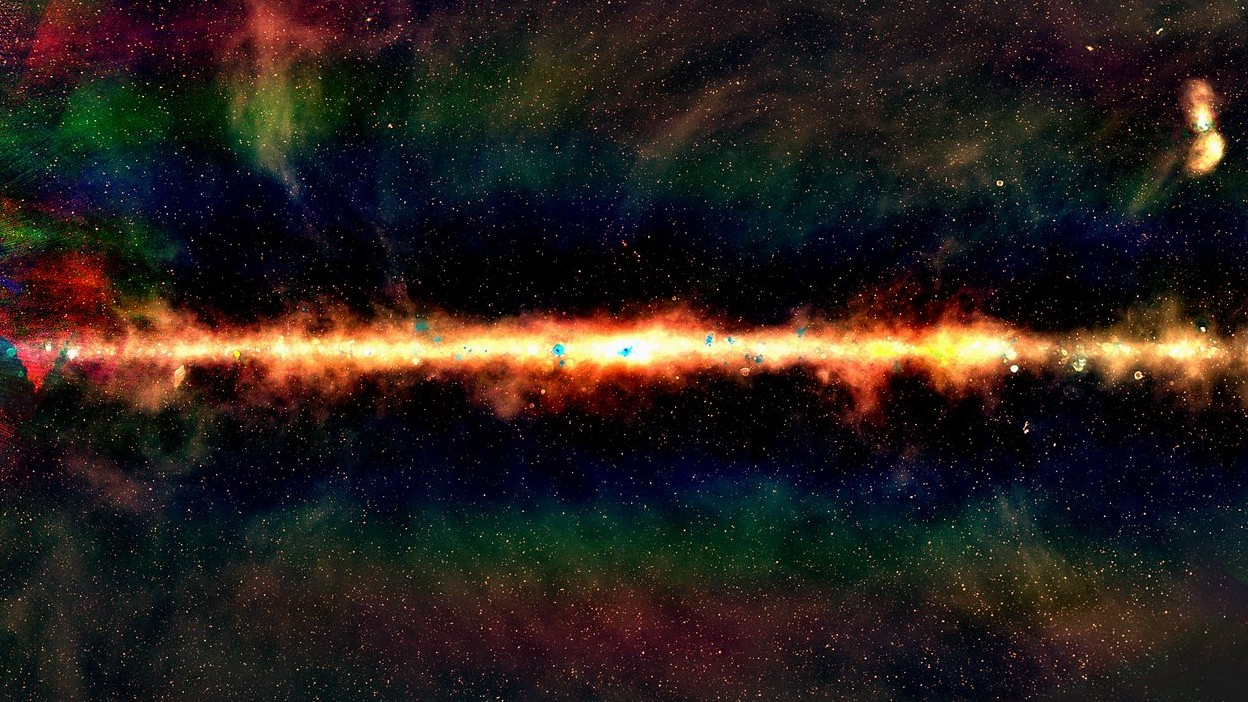
\includegraphics[width=\textwidth]{images/gleam.jpg}
        \caption{\label{fig:gleam} False-colour image of the radio sky from the GLEAM survey. (Image: Natasha Hurley-Walker, Curtin University/ICRAR \citeneeded)}
    \end{figure}

\section{Astrophysics of Extended Radio Sources}
\label{sec:physics-of-radio-sources}

    % In this section I'll talk about extended radio sources: AGN, their jets, and the unified model as described by Urry and Padovani. I'll need to talk about synchrotron radiation and the AGN core and jets. It'd also make sense to talk about observational classes, including FRI and FRII, and how orientation affects this. How do radio objects evolve over time? What are the main questions in the field?

    The extragalactic sky appears quite different at different wavelengths. While an optical observer may look at a distant galaxy and see spirals and halos, an infrared observer will see discs and dust. What does the radio astronomer see? 

    \autoref{fig:gleam} shows a false-colour image of the radio sky. The disc of the Milky Way is clearly visible through the center, but nearly every other object in this image is a galaxy. These galaxies fall into two main categories: those that emit radio due to star formation, and those that emit radio due to \defn{active galactic nuclei} (AGN). Since star formation is limited to the galaxy proper (usually within tens of kiloparsecs of the galaxy centre), and the resolution of wide radio surveys tends to be upwards of 5 arcseconds, most star forming galaxies appear unresolved in radio, and the extended sources are dominated by AGN.

    AGN are some of the most energetic objects in the Universe. They both provide a laboratory for extreme physics and are a key part of the life cycle of a galaxy \citep{heckman_coevolution_2014}. Powered by a supermassive black hole, they convert gravitational potential energy into intense electromagnetic radiation at a broad range of frequencies. AGN that produce strong radio emission are called radio AGN, and methods of observing the complex structures that these radio AGN form will be the focus of this thesis.

    \subsection{Active galactic nuclei}
    \label{sec:agn}

        \begin{figure}
            \centering
            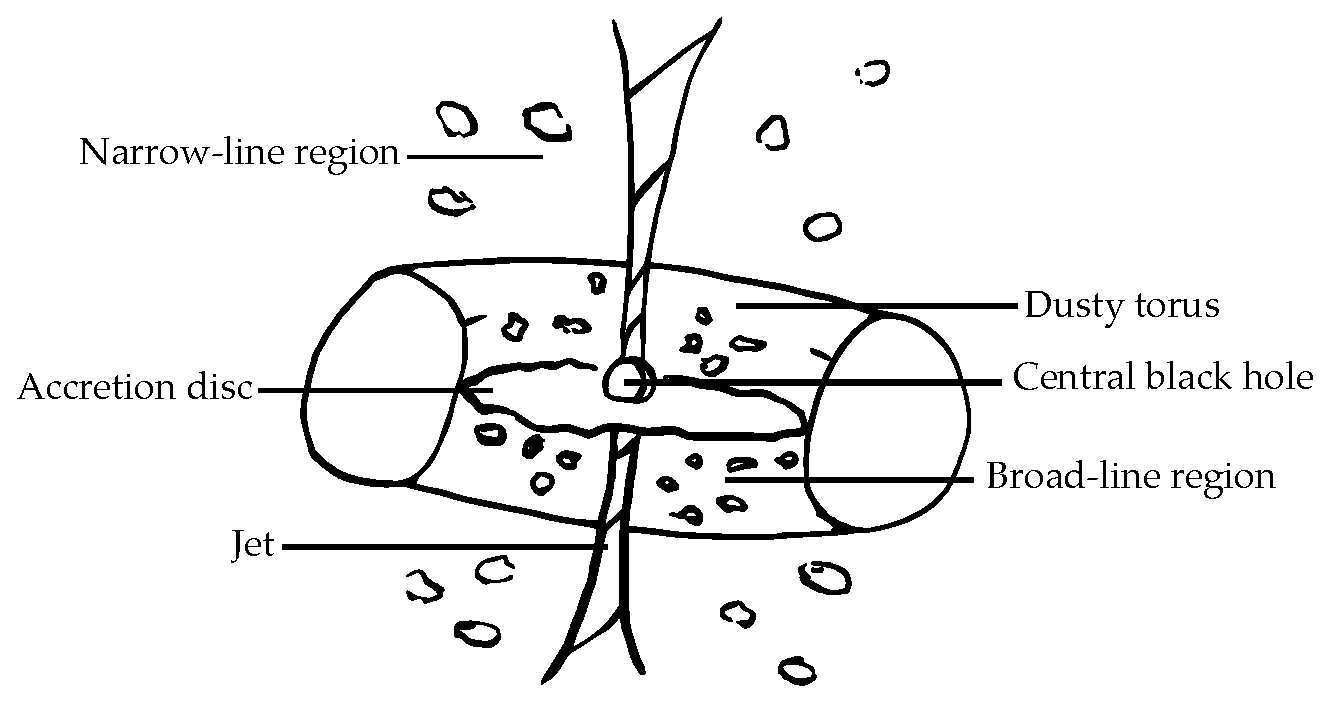
\includegraphics[width=\textwidth]{images/agn.eps}
            \caption{\label{fig:agn} The unified model of AGN.}
        \end{figure}

        At their core, AGN are an accreting \defn{supermassive black hole}: a body so dense that even light cannot escape its gravitational pull, with mass on the order of $10^7$--$10^9\ \mathrm{M}_\odot$ \citeneeded{}. Such black holes seem to exist at the centre of galaxies\citeneeded{} and these galaxies are called \defn{host galaxies}. The current understanding of the structure of an AGN is as follows \citep{urry_unified_1995}. The black hole is surrounded by an accretion disc emitting in ultraviolet and X-ray. Beyond this is the broad-line region, named for the broad emission lines emitted by clouds of material surrounding the accretion disc. The broad-line region and accretion disc are themselves surrounded by a dusty torus (or some other disc-like structure) which prevents light from the centre of the AGN being observed from the sides. Further still from the accretion disc is the narrow-line region, where lower-energy gas produces narrow emission lines. From either side of the disc, an AGN produces two collimated outflows of relativistic plasma called {jets}, and these jets interact with gas in the host galaxy to produce bright radio emission. As the jets disperse further out from the centre of the AGN they widen into plumes of plasma known as \defn{lobes}. This model of AGN unifies different observed classes of AGN by their orientation and luminosity, and is hence known as the \defn{unified model} \citep{antonucci_unified_1993}.

        There are many different ways to divide the set of radio AGN into classes. By morphology, radio AGN are often divided by the structure of the jets and lobes: Fanaroff-Riley type I (FRI) and Fanaroff-Riley type II (FRII) are the most striking examples, with FRI having wavy, diffuse lobes; and FRII having long, tightly-collimated jets and sharp-edged lobes with bright hot-spots \citep{urry_unified_1995}. FRII are also generally higher-luminosity \citep{fanaroff_morphology_1974} than FRI and therefore make up the majority of observed extended radio sources throughout the Universe. AGN can also be divided into \defn{radiative-mode} and \defn{jet-mode} by how they expel their energy \citep{heckman_coevolution_2014}. Radiative-mode AGN produce radiative energy in amounts higher than 1 percent of their Eddington limit, while jet-mode AGN mainly output energy through their jets. The Eddington limit describes the maximum luminosity that a compact object can emit, and is given in \autoref{eq:eddington} \citep{rybicki_radiative_1979}:
        \begin{equation}
            L_{\mathrm{Eddington}}(M) = \frac{4\pi G M m_p c}{\sigma_T}.
            \label{eq:eddington}
        \end{equation}
        Optical emission observed near the centre of the AGN can be used to divide radio AGN into broad-line and narrow-line galaxies: the former are AGN seen end-on, and the latter are AGN seen edge-on with the dusty torus obscuring the broad-line region and are the only ones for which we see significant extended structure.

        The jets and lobes of AGN can be very extended, with the largest known radio galaxies measuring over 4 Mpc end-to-end \citep{machalski_understanding_2011}. This is much larger than the radius of their host galaxies, and so the jets and lobes of AGN are uniquely posed to interact with the local environment. Environmental interactions both within and outside the host galaxy warp and distort the jets and lobes and lead to a great variety of exotic-shaped radio galaxies.

    \subsection{Radio emission from AGN}
        
        Most radio emission from AGN is \defn{synchrotron radiation}, produced by relativistic charged particles accelerating in a magnetic field. A non-relativistic charged particle will spiral with a fixed angular frequency when it moves in a magnetic field in a process called \defn{gyro radiation}. Synchrotron radiation is a relativistic effect: it can be thought of as gyro radiation Lorentz transformed to energies much greater than $mc^2$. The spectrum of synchrotron radiation follows a power law \citep{condon_essential_2016}:
        \begin{equation}
            \label{eq:spectral-index}
            S(\nu) \propto \nu^{\alpha}.
        \end{equation}
        $\alpha$ is called the \defn{spectral index}\footnote{Note that the sign of $\alpha$ varies by convention, and both $S \propto \nu^{\alpha}$ and $S \propto \nu^{-\alpha}$ exist in the literature.}. It is related to the energy distribution of the emitting electrons: assuming that the electron energy distribution follows a power law (which it generally does\citeneeded), where the number density of electrons at a given energy $E$ is given by
        \begin{equation}
            n(E) \propto E^\Gamma,
        \end{equation}
        then
        \begin{equation}
            \alpha = \frac{\Gamma - 1}{2}.
        \end{equation}
        AGN cores tend to have spectral indices around -0.7 \citeneeded, while the spectral index of the lobes is higher \citeneeded.

        % The most general form of the electric field in an electromagnetic wave, propagating in the $\hat z$ direction, is
        % \begin{equation}
        %     \vec E = (\hat x E_x \exp^{i\varphi_x} + \hat y E_y \exp^{i\varphi_y}) e^{i(k \hat z \cdot \vec r - \omega t)}
        % \end{equation}
        % where $\vec r$ is the position vector and $k$ is the \defn{wavenumber}. This is the composition of two orthogonal waves

        \subsubsection{Polarisation}
        \label{sec:polarisation}

            \todo{This section is kinda terrible! Rewrite to be in terms of two orthogonal waves (-> linear polarisation) and if these are out of phase we have circular polarisation. Introduce the Poincar\'e sphere or at least an ellipse?}
            An electromagnetic wave travels at an angle. This angle and its behaviour is called the \defn{polarisation} of the wave. As this wave propagates along the line-of-sight toward an observer, the electric field oscillates in an ellipse across the plane. This ellipse can be characterised by the \defn{Stokes parameters}. Split the electric field $\vec E$ along the $x$--$y$ plane perpendicular to the line-of-sight $\hat z$ into two orthogonal components $E_x$ and $E_y$:
            \begin{equation}
                \vec E = (\hat x E_x \exp(i \varphi_x) + \hat y E_y \exp(i \varphi_y)) \exp(i (\vec k \cdot \hat z - \omega t)).
            \end{equation}
            $\vec k$ is the \defn{wave vector} which points in the direction of travel and has magnitude $2\pi/\lambda$ and $\omega = 2\pi\nu$ is the \defn{angular frequency}. $\varphi_x$ and $\varphi_y$ are the phase offsets of each component. The Stokes parameters are then \citep{condon_essential_2016}
            \begin{align}
                \label{eq:stokes-i}
                I &= \frac{1}{R_0} \mathbb E_t[E_x^2 + E_y^2],\\
                \label{eq:stokes-q}
                Q &= \frac{1}{R_0} \mathbb E_t[E_x^2 - E_y^2],\\
                \label{eq:stokes-u}
                U &= \frac{1}{R_0} \mathbb E_t[2 E_x^2 E_y^2 \cos (\varphi_x - \varphi_y)],\\
                \label{eq:stokes-v}
                V &= \frac{1}{R_0} \mathbb E_t[2 E_x^2 E_y^2 \sin (\varphi_x - \varphi_y)].
            \end{align}
            $I$ is the \defn{total intensity}. $Q$ and $U$ together describe the \defn{linear polarisation}, which is related to the angle of the ellipse described above, called the \defn{polarisation angle} $\chi$:
            \begin{equation}
                \label{eq:polarisation-angle}
                \tan (2 \chi) = \frac{U}{Q}.
            \end{equation}
            $V$ is called the \defn{circular polarisation} and describes the eccentricity of this ellipse. For most extragalactic sources, the circular polarisation is zero \citeneeded because \todo{reasons}. The polarised intensity is
            \begin{equation}
                \label{eq:polarised-intensity}
                P^2 = Q^2 + U^2 + V^2.
            \end{equation}
            Note that $P^2 \leq I^2$. The \defn{fractional polarisation} is the ratio between these two intensities:
            \begin{equation}
                p = \frac{P}{I}.
            \end{equation}

            The synchrotron radiation from AGN is polarised, though this polarisation is not always detectable \citeneeded \todo{forward reference to the next section?}. Additionally, the most common non-AGN cause for radio emission is star-formation, which does not have detectable polarisation. Polarisation is therefore an excellent way to confirm that a radio source is an AGN.

            Polarisation can also be used to describe the magnetic structure of both AGN and intervening medium.

        % Following \citet{condon_essential_2016}, we will derive the expected power spectrum of synchrotron radiation. A \emph{non-}relativistic charged particle moving at velocity $\vec v$ in a magnetic field $\vec B$ is subject to the Lorentz force $\vec F$:
        % \begin{equation}
        %     \vec F = q \vec v \times \vec B.
        % \end{equation}
        % The Lorentz force causes the particle to spiral with a fixed angular frequency independent of its speed:
        % \begin{equation}
        %     \label{eq:angular-gyro-frequency}
        %     \omega_G = \frac{qB}{m}.
        % \end{equation}
        % Such a particle will emit \defn{gyro radiation} at the \defn{gyro frequency} $\nu_G = \omega_G/2\pi$. Synchrotron radiation is gyro radiation Lorentz transformed to energies much greater than $mc^2$. The power emitted by gyro radiation is given by Larmor's equation:
        % \begin{equation}
        %     \label{eq:larmor}
        %     P = \frac{2}{3} \frac{1}{4\pi\epsilon_0} \frac{q^2}{c^3} \dot v_\perp^2
        % \end{equation}
        % where $\dot v_\perp$ is the component of the particle's acceleration perpendicular to the magnetic field. Transform coordinates to the rest frame of the magnetic field:
        % \begin{equation}
        %     \dot v_\perp \to \gamma^2 \dot v_\perp, P \to P
        % \end{equation}
        % where $\gamma$ is the Lorentz factor
        % \begin{equation}
        %     \gamma = \frac{1}{\sqrt{1 - \frac{v^2}{c^2}}}.
        %     \label{sec:lorentz-factor}
        % \end{equation}
        % This gives the observed power of synchrotron radiation for a charged particle:
        % \begin{equation}
        %     \label{eq:larmor-boosted}
        %     P = \frac{2}{3} \frac{1}{4\pi\epsilon_0} \frac{q^2\gamma^4}{c^3} \dot v_\perp^2.
        % \end{equation}
        % It remains to find $\dot v_\perp^2$ in terms of the magnetic field. The acceleration for a relativistic orbiting particle is
        % \begin{equation}
        %     \dot v_\perp = \frac{\omega_G}{\gamma} v_\perp
        % \end{equation}
        % and substituting the angular gyro frequency (\autoref{eq:angular-gyro-frequency}) gives
        % \begin{equation}
        %     \dot v_\perp = \frac{qB}{m\gamma} v_\perp = \frac{q}{m\gamma} |\vec v \times \vec B|.
        % \end{equation}
        % This can then be substituted into \autoref{eq:larmor-boosted} to obtain the synchrotron power radiated by a single charged particle:
        % \begin{equation}
        %     \label{eq:synchrotron-radiation-single}
        %     P = \frac{2}{3} \frac{1}{4\pi\epsilon_0} \frac{q^4 \gamma^2}{m^2 c^3} (\vec v \times \vec B)^2.
        % \end{equation}
        % For an electron, we can let $q = q_e$ and $m = m_e$ and write the power in terms of the Thomson cross-section $\sigma_T$:
        % \begin{equation}
        %     \label{eq:synchrotron-radiation-single-thomson}
        %     P = \epsilon_0 \sigma_T c \gamma^2 (\vec v \times \vec B)^2
        % \end{equation}
        % noting that
        % \begin{equation}
        %     \label{eq:thomson-cross-section}
        %     \sigma_T = \frac{8\pi}{3} \left(\frac{1}{4\pi\epsilon_0} \frac{e^2}{m_e c^2}\right)^2.
        % \end{equation}
        % Assuming an isotropic distribution of electrons in a plasma, we can integrate over all angles to find the average synchrotron power emitted by a single electron:
        % \begin{equation}
        %     \label{eq:average-single-synchrotron-power}
        %     \mathbb{E}[P] = \frac{2}{3} \epsilon_0 \sigma_T c \gamma^2 vB
        % \end{equation}
        % We can use this to find the expected power spectrum of synchrotron radiation from an ensemble of electrons. Assuming that the electrons follow a power law energy distribution (which they generally do\citeneeded), the number density of electrons at a given energy $E$ is
        % \begin{equation}
        %     n(E) \propto E^{-\delta}
        % \end{equation}
        % where $\delta$ is a constant. Further assuming that each electron radiates at the frequency $\gamma^2 \nu_G$, then 


\section{Observing Radio Sources}
\label{sec:radio-astronomy}

This section needs to talk about how the physics of AGN affects observations and what kind of data we deal with. I'll need to talk about radio telescopes, Fourier transforms, and the noise properties of radio sources, as well as what kind of sources we expect to find throughout the universe. How do observations limit our understanding of AGN? How do observational effects change what we see? What are the main difficulties in radio astronomy?


\section{Machine Learning for Radio Astroninformatics}
\label{sec:radio-astroinformatics}

% Here we need to talk about the fundamentals of machine learning. We'll start with problem formulations and what machine learning is, then discuss terminology and classification. We need to cover the difficulties of labels and the lack of groundtruth in astronomy, the problem and handling of uncertainties, and feature selection. We also need to talk about the importance (or unimportance?) of interpretability and how this ties into astronomy, and the unique idea of using machine learning as a pathway to understand something important about physics.

    Machine learning was once described to me by an anonymous supervisor as ``the statistics kept at the back of the textbook''. But even accepting its grounding in statistics, is this really an accurate description of the field? I think of machine learning as a data-driven way of formalising predictive problems mathematically, converting between different kinds of statistical problems, and an accompanying set of methods and practices for handling data and uncertainty. The eventual goal is to design some method or algorithm that automatically discovers useful information in (potentially very large) data sets. The machine learning component of this thesis will require an understanding of linear algebra, probability, statistics, and vector calculus. I will begin describing machine learning by exploring the concept of a predictor.
    % \citet{deisenroth_mathematics_2020} seperate machine learning into three core components: the data, the model, and learning.

    \subsection{Predictors}
    \label{sec:predictors}

        A \defn{predictor} is some function that produces an output from some given input. They can be represented as functions or as probabilistic models, depending on the machine learning approach being undertaken. As a function, a predictor maps from some input domain $\mathcal X$ into some output domain $\mathcal Y$, and is usually written as
        \begin{equation}
            f : \mathcal X \to \mathcal Y.
        \end{equation}
        $\mathcal X$ and $\mathcal Y$ are commonly (but certainly not always) a real vector space $\mathbb R^n$. Because the goal of machine learning involves \emph{finding} a suitable function $f$ for the task at hand, the set of functions is usually constrained. For example, if $\mathcal X = \mathbb{R}^n$, we might require that $f$ is a linear function $\mathbb R^n \to \mathbb R$, easily parametrised by $n + 1$ constants.

        As a probabilistic model, a predictor is a joint probability distribution between observations and hidden parameters \citep{deisenroth_mathematics_2020}. Using a probabilistic predictor allows us to formally describe and work with uncertainty both in the input space and output space. Such a predictor is usually parametrised by a finite set of parameters, which already includes most common probability distributions.

    \subsection{Data and representation}
    \label{sec:data-and-representation}

        Machine learning is centred on data and the extraction of information from that data. Data can include anything from numeric information, documents, or images to spectra or galaxies. A collection of data is called a \defn{dataset} and an element of this dataset is (interchangably) called an \defn{example} or \defn{instance}. Generally, data are not easy to work with in their original form and must be converted into a numerical representation before use. As it is relatively easy to work with both numerically and analytically, we usually convert our data into real vectors in $\mathbb R^n$. Each axis of this vector space is called a \defn{feature}. Features are non-trivial to choose, and finding good features often requires the expertise of a human who is well-versed in the original dataset (a \defn{domain expert}).

        % This conversion is called an \defn{embedding} of that data into a space. One way to embed data into a vector space is to use real numbers representative of different features and details of the original data. These values are called \defn{features} and the resulting embedding is called a \defn{feature representation}. 

    % There are many sub-fields of machine learning, divided mainly by the kind of predictions required. The most important sub-field that we will use in this thesis is classification.

    \subsection{Classification}
    \label{sec:classification}

        \defn{Classification} is the problem of categorising objects into classes. 
%!tex root=./thesis.tex
\chapter{Radio Cross-identification}
\label{cha:cross-id}

    % a. introduction and motivation
    % b. binary cross-identification
    % c. crowdsourced data and radio galaxy zoo
    % d. results (from ATLAS and FIRST)
    % e. basically the entire ATLAS paper

This chapter is based on my paper \emph{Radio Galaxy Zoo: Machine learning for radio source host galaxy cross-identification}, by M. J. Alger, J. K. Banfield, C. S. Ong, L. Rudnick, O. I. Wong, C. Wolf, H. Andernach, R. P. Norris, and S. S. Shabala; published in the \emph{Monthly Notices of the Royal Astronomical Society} in 2018. Some minor changes have been made to match the rest of this thesis.\\

In this chapter, we consider the problem of determining the host galaxies of radio sources by cross-identification. This has traditionally been done manually, which will be intractable for upcoming and ongoing wide-area radio surveys like the Evolutionary Map of the Universe (EMU). {Automated cross-identification will be critical for these future surveys, and machine learning may provide the tools to develop such methods.

We applied a standard approach from computer vision to cross-identification, introducing one possible way of automating this problem, and explored the pros and cons of this approach}. We applied our method to the $1.4$~GHz Australian Telescope Large Area Survey (ATLAS) observations of the \emph{Chandra} Deep Field South (CDFS) and the ESO Large Area ISO Survey South 1 (ELAIS-S1) fields by cross-identifying them with the \emph{Spitzer} Wide-area Infrared Extragalactic (SWIRE) survey. We trained our method with two sets of data: expert cross-identifications of CDFS from the initial ATLAS data release and crowdsourced cross-identifications of CDFS from Radio Galaxy Zoo. {We found that a simple strategy of cross-identifying a radio component with the nearest galaxy performs comparably to our more complex methods, though our estimated best-case performance is near 100 per cent. ATLAS contains 87 complex radio sources that have been cross-identified by experts, so there are not enough complex examples to learn how to cross-identify them accurately. Much larger datasets are therefore required for training methods like ours. We also showed that training our method on Radio Galaxy Zoo cross-identifications gives comparable results to training on expert cross-identifications, demonstrating the value of crowdsourced training data.}

\section{Introduction to cross-identification}
\label{sec:atlas-xid-intro-cross-id}

    \begin{figure}
        \centering
        \begin{subfigure}{0.3\textwidth}
            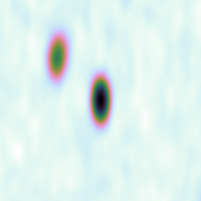
\includegraphics[width=\textwidth]{atlas-images/cdfs_100_compact.png}
            \caption{\raggedright{} Two compact components, each a compact source.}
        \end{subfigure}
        \begin{subfigure}{0.3\textwidth}
            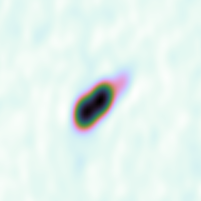
\includegraphics[width=\textwidth]{atlas-images/elais_57_resolved.png}
            \caption{\raggedright{} One resolved component and resolved source.}
        \end{subfigure}
        \begin{subfigure}{0.3\textwidth}
            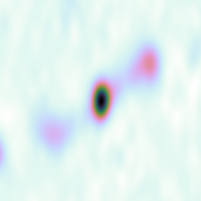
\includegraphics[width=\textwidth]{atlas-images/cdfs_185_resolved.png}
            \caption{\raggedright{} Three resolved components comprising one resolved source.}
        \end{subfigure}
        \caption[Examples showing key definitions of radio emission regions used throughout this chapter.]{\label{fig:definitions} Examples showing key definitions of radio emission regions used throughout this chapter.
                 Compact and resolved components are defined by \autoref{eq:atlas-compact}.}
    \end{figure}

    Next generation radio telescopes such as the Australian SKA Pathfinder \citep[ASKAP;][]{johnston07} and Apertif \citep{verheijen08} will conduct increasingly wide, deep, and high-resolution radio surveys, producing large amounts of data. The Evolutionary Map of the Universe \citep[EMU;][]{norris11} survey using ASKAP is expected to detect over 70 million radio sources, compared to the 2.5 million radio sources currently known \citep{banfield15}. An important part of processing these data is cross-identifying observed radio emission regions with observations of their host galaxies in surveys at other wavelengths.

    In the presence of extended radio emission, cross-identification of the host can be a
    difficult task. {Radio emission may extend far from the host galaxy
    and emission regions from a single physical object may appear disconnected. As a result, the
    observed structure of a radio source may have a complex relationship
    with the corresponding host galaxy, and cross-identification in radio is
    much more difficult than cross-identification at shorter wavelengths.} Small surveys
    containing a few thousand sources such as the Australia Telescope Large Area Survey
    \citep[ATLAS;][]{norris06, middelberg08} can be cross-identified manually,
    but this is impractical for larger surveys.

    One approach to cross-identification of large numbers of sources is crowdsourcing, where volunteers
    cross-identify radio sources with their host galaxies. This is the premise of Radio Galaxy
    Zoo\footnote{\url{https://radio.galaxyzoo.org}} \citep{banfield15}, a
    citizen science project hosted on the Zooniverse platform \citep{lintott08}.
    Volunteers are shown radio and infrared images and are asked to
    cross-identify radio sources with the corresponding infrared host galaxies. An
    explanation of the project can be found in \citet{banfield15}. The first
    data release for Radio Galaxy Zoo will provide a large dataset of over
    75~000 radio-host cross-identifications and radio source morphologies
    (Wong et al., in prep.). While this is a much larger number of visual
    cross-identifications than have been made by experts \citep[e.g.,
    ][]{taylor2007,Gendre2008,grant2010,norris06,middelberg08} it is still far
    short of the millions of radio sources expected to be detected in upcoming
    radio surveys \citep{norris17surveys}.

    Automated algorithms have been developed for cross-identification.
    \citet{fan15} applied Bayesian
    hypothesis testing to this problem, fitting a three-component model to extended radio
    sources. This was achieved under the assumption that extended radio sources
    are composed of a core radio component and two lobe components. The core
    radio component is coincident with the host galaxy, so cross-identification
    amounts to finding the galaxy coincident with the core radio component in
    the most likely model fit. This method could easily be extended to use other, more
    complex models, but it is purely geometric. It does not incorporate
    other information such as the physical properties of the potential host
    galaxy. Additionally, there may be new classes of radio source detected in
    future surveys like EMU which do not fit the model. \citet{weston18lrpy}
    developed a modification of the likelihood ratio method of
    cross-identification \citep{richter75likelihood} for application to ATLAS
    and EMU. This method does well on non-extended radio sources
    with approximately 70 per cent accuracy in the ATLAS fields, but does
    not currently handle more complex (extended or multi-component) radio sources
    \citep{norris17unexpected}.

    {One possibility is that machine learning techniques can
    be developed to automatically cross-identify catalogues drawn from new surveys}. Machine learning
    describes a class of methods that learn approximations to functions. {If
    cross-identification can be cast as a function approximation problem, then machine learning will allow datasets
    such as Radio Galaxy Zoo to be generalised to work on new data. Datasets from
    citizen scientists have already been used to train machine learning methods.
    Some astronomical examples can be found in \citet{marshall15citizen}.}

    In this chapter we {cast cross-identification as a function
    approximation problem by} applying an approach from computer vision
    literature. This approach casts cross-identification as the standard machine
    learning problem of binary classification {by asking whether a given
    infrared source is the host galaxy or not}. We train our methods on expert
    cross-identifications and volunteer cross-identifications from Radio Galaxy Zoo. In
    \autoref{sec:atlas-xid-data} we describe the data we use to train our methods. In
    \autoref{sec:atlas-xid-method} we discuss how we cast the radio host galaxy
    cross-identification problem as a machine learning problem. In
    \autoref{sec:atlas-xid-results} we present results of applying our method to ATLAS
    observations of the \emph{Chandra} Deep Field South (CDFS) and the ESO Large Area ISO Survey South 1 (ELAIS-S1) field. Our data, code and results are
    available at \url{https://radiogalaxyzoo.github.io/atlas-xid}.

    {Throughout this chapter, a `radio source' refers to all radio emission observed associated with a single host galaxy, and a `radio component' refers to a single, contiguous
    region of radio emission. Multiple components may arise from a single
    source. A `compact' source is composed of a {single unresolved component. \autoref{eq:atlas-compact} shows the definition of a resolved component. We
    assume that all unresolved components are compact sources, i.e. we assume that each unresolved component has its own host galaxy\footnote{{This will be incorrect if the unresolved components are actually compact lobes or hot-spots, but determining which components correspond to unique radio sources is outside the scope of this thesis.}}.} An `extended'
    source is a non-compact source, i.e. resolved single-component sources or a
    multi-component source. \autoref{fig:definitions} illustrates these definitions.}

\section{Data}\label{sec:atlas-xid-data}

  We use radio data from the Australia Telescope Large Area Survey
  \citep[ATLAS;][]{norris06,franzen15}, infrared data from the \emph{Spitzer}
  Wide-area Infrared Extragalactic survey \citep[SWIRE;][]{lonsdale03swire,
  surace05swire}, and cross-identifications of these surveys from the citizen
  science project Radio Galaxy Zoo \citep{banfield15}. Radio Galaxy Zoo also
  includes cross-identifications of sources in Faint Images of the Radio Sky at
  Twenty Centimeters \citep[FIRST;][]{white97first} and the All\emph{WISE}
  survey \citep{cutri2013wiseexplanatory}, though we focus only on Radio
  Galaxy Zoo data from ATLAS and SWIRE.

  \subsection{ATLAS}\label{sec:atlas-xid-atlas}
    \begin{table}
      \caption[Catalogues of ATLAS/SWIRE cross-identifications for the CDFS
        and ELAIS-S1 fields.]{Catalogues of ATLAS/SWIRE cross-identifications for the CDFS
        and ELAIS-S1 fields. The method used to generate each catalogue is
        shown, along with the number of radio components cross-identified in each
        field.}
      \centering
      \label{tab:atlas-cids}
      \begin{tabular}{llcc}
        \hline\hline
        Catalogue & Method & CDFS & ELAIS-S1\\
        \hline
        \citet{norris06} & Manual & 784 & 0\\
        \citet{middelberg08} & Manual & 0 & 1366\\
        \citet{fan15} & Bayesian models & 784 & 0\\
        \citet{weston18lrpy} & Likelihood ratio & 3078 & 2113\\
        Wong et al. (in prep.) & Crowdsourcing & 2460 & 0 \\
        \hline\hline
      \end{tabular}
    \end{table}

    ATLAS is a pilot survey for the EMU \citep{norris11} survey, which will
    cover the entire sky south of $+30$ deg and is expected to detect
    approximately 70 million new radio sources. {95 per cent of these sources
    will be single-component sources, but the remaining 5 per cent pose a
    considerable challenge to current automated cross-identification methods
    \citep{norris11}.} EMU will be conducted at the same depth and resolution
    as ATLAS, so methods developed for processing ATLAS data are expected to
    work for EMU. ATLAS is a wide-area radio survey of the CDFS and ELAIS-S1
    fields at 1.4~GHz with a sensitivity of 14 and
    \unit{17}{\micro\jansky}~beam$^{-1}$ on CDFS and ELAIS-S1 respectively.
    CDFS covers 3.6~deg$^2$ and contains 3034 radio components above a
    signal-to-noise ratio of 5. ELAIS-S1 covers 2.7~deg$^2$ and contains 2084
    radio components above a signal-to-noise ratio of 5 \citep{franzen15}. The
    images of CDFS and ELAIS-S1 have angular resolutions of 16 by 7 and 12 by
    8 arcsec respectively, with pixel sizes of 1.5 arcsec px$^{-1}$.
    \autoref{tab:atlas-cids} summarises catalogues that contain
    cross-identifications of radio components in ATLAS with host galaxies in
    SWIRE. In the present work, we train methods on
    CDFS\footnote{{Radio Galaxy Zoo only contains CDFS sources and so
    we cannot train methods on ELAIS-S1.}} and test these methods on both CDFS
    and ELAIS-S1. This helps confirm that our methods are transferable to different
    areas of the sky observed by the same telescope, as will be the case for
    EMU.

  \subsection{SWIRE}\label{sec:atlas-xid-swire}

    SWIRE is a wide-area infrared
    survey at the four IRAC wavelengths 3.6, 4.5, 5.8, and
    \unit{8.0}{\micro\meter} \citep{lonsdale03swire, surace05swire}. It covers eight fields, including CDFS and ELAIS-S1. SWIRE is the source of infrared
    observations for cross-identification with ATLAS. SWIRE has catalogued 221,535
    infrared objects in CDFS and 186,059 infrared objects in ELAIS-S1 above a signal-to-noise ratio of 5.

  \subsection{Radio Galaxy Zoo}\label{sec:atlas-xid-rgz}

    Radio Galaxy Zoo asks volunteers to cross-identify radio components with
    their infrared host galaxies. There are a total of 2460 radio components
    in Radio Galaxy Zoo sourced from ATLAS {observations of CDFS}. These components are
    cross-identified by Radio Galaxy Zoo participants with host galaxies
    detected in SWIRE. A more detailed description can be found in
    \citet{banfield15} and a full description of how the Radio Galaxy Zoo catalogue used in this work\footnote{The Radio Galaxy Zoo Data
    Release 1 catalogue will only include cross-identifications for which over
    65 per cent of volunteers agree. However, we use a preliminary catalogue containing volunteer
    cross-identifications for all components.} is generated can be found in Wong
    et al. (in prep.).

    The ATLAS~CDFS radio components that appear in Radio Galaxy Zoo {are drawn from a prerelease version of} the third data release
    of ATLAS by \citet{franzen15}. In this release, each radio component was fit with a
    two-dimensional Gaussian. Depending on the residual of the fit, more than
    one Gaussian may be fit to one region of radio emission. Each of these
    Gaussian fits is listed as a radio component in the ATLAS component catalogue. The
    brightest radio component from the multiple-Gaussian fit is called the
    `primary component'. {If there is only one Gaussian fit then this Gaussian is the primary component}. Each primary component found in the ATLAS
    component catalogue appears in Radio Galaxy Zoo. Non-primary components
    may appear within the image of a primary component, but do not have their
    own entry in Radio Galaxy Zoo. We will henceforth only discuss the primary
    components.

  \section{Method}\label{sec:atlas-xid-method}
    \begin{figure}
      \centering
      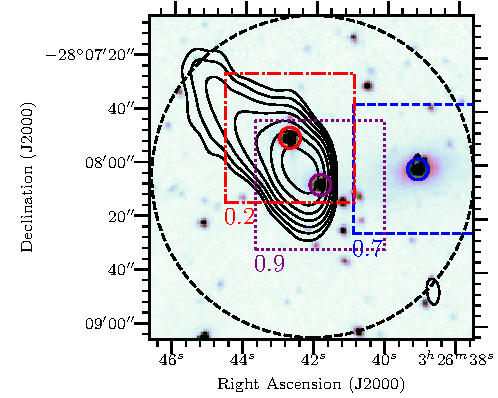
\includegraphics[width=0.6\columnwidth]{atlas-images/figure_example_of_method.pdf}
      \caption[An example of {finding} the host galaxy of a radio source using
        our sliding-window method.]{An example of {finding} the host galaxy of a radio source using
        our sliding-window method. The background image is a \unit{3.6}{\micro\meter} image from SWIRE. The contours show ATLAS radio data and start at $4\sigma$, increasing geometrically by a factor of 2. Boxes represent `windows'
        centred on {candidate host galaxies, which are circled. The pixels in each window are used to represent the candidate that the window is centred
        on. The scores of each candidate would be calculated by a binary classifier using the window as input,
        and these scores are shown below each window}. The scores
        shown are for illustration only. In this example,
        {the galaxy coincident with the centre window would be chosen as the host galaxy, as this
        window has the highest score.
        The dashed circle
        shows the $1'$ radius from which candidate host galaxies are selected. For clarity, not all candidate host galaxies are shown.}}
      \label{fig:windows}
    \end{figure}

  {The aim of this chapter is to express cross-identification in a form that
  will allow us to apply standard machine learning tools and methods. We use an approach from computer vision
  to cast cross-identification as binary classification.}

  \subsection{Cross-identification as binary classification}\label{sec:atlas-xid-as-binary-classification}
    \begin{figure}
      \centering
      %
      \tikzstyle{decision} = [diamond, draw, fill=white,
          text width=4.5em, text badly centered, inner sep=0pt]
      \tikzstyle{block} = [rectangle, draw, fill=white,
          text width=5em, text centered, rounded corners, minimum height=4em]
      \tikzstyle{line} = [draw, -latex']
      \begin{tikzpicture}[node distance=6mm, auto]
        \node [block] (init) {input radio source};
        \node [decision, right= of init] (iscompact) {compact?};
        \node [block, below= of iscompact] (compact) {find nearest infrared object};
        \node [block, right= of iscompact] (resolved) {find nearby infrared objects};
        \node [block, fill=black!30, right= of resolved] (classify) {classify objects};
        \node [block, below= of classify] (best) {choose object based on {score}};
        \coordinate (middle) at ($(compact)!0.5!(best)$);
        \node [block, below= of middle, fill=green!40] (done) {\textbf{host galaxy}};
        \path [line] (init) -- (iscompact);
        \path [line] (iscompact) -- (compact) node [midway] {yes};
        \path [line] (compact) -- (done);
        \path [line] (iscompact) -- (resolved) node [midway] {no};
        \path [line] (resolved) -- (classify);
        \path [line] (classify) -- (best);
        \path [line] (best) -- (done);
      \end{tikzpicture}
      \caption[Our cross-identification method once a binary classifier has been trained.]{{Our cross-identification method once a binary classifier has been trained}. As
        input we accept a radio {component. If the component is compact, we assume it is a compact source and select
        the nearest infrared object as the host galaxy. If the component is
        resolved, we use the binary classifier to score all nearby infrared objects
        and select the highest-scored object as the host galaxy. Compact and resolved components are defined in \autoref{eq:atlas-compact}.}}
      \label{fig:flowchart}
    \end{figure}

    We propose a two-step method for host galaxy cross-identification
    {which we will describe now}. Given a radio component, we want to find
    the corresponding host galaxy. The input is a $2' \times
    2'$ radio image of
    the sky centred on a radio component {and potentially other information about
    objects in the image (such as the redshift or infrared colour)}. {Images at other wavelengths (notably infrared) might be
    useful, but we defer this for now as it complicates the task.
    {We choose a $2' \times 2'$ image to match} the size of the images used
    by Radio Galaxy Zoo. To avoid solving the separate task of identifying
    which radio components are associated with the same source, we assume
    that each radio image represents a single extended
    source\footnote{Limitations of this assumption are discussed in
    \autoref{sec:atlas-xid-limitations}.}. Radio cross-identification can then
    be formalised as follows: Given a radio image centred on a radio
    component, locate the host galaxy of the source containing this radio
    component. This is a standard computer vision problem called `object
    detection', and we apply a common technique called a `sliding-window'
    \citep{rowley1996facedetection}}.

    {In sliding-window object detection, we want to find an object in an image.
    We develop a function to score each location in the image such that the
    highest-scored location coincides with the desired object. Square image
    cutouts called `windows' are taken centred on each location and these
    windows are used to represent that location in our scoring function. To
    find the infrared host galaxy, we choose the location with the highest
    score. To improve the efficiency of this process when applied to
    cross-identification, we only consider windows coincident with infrared
    sources detected in SWIRE. We call these infrared sources `candidate
    host galaxies'. For this chapter, there is no use in scoring
    locations without infrared sources as that would not lead to a host identification
    anyway. Using candidate host galaxies instead of pixels also
    allows us to include ancillary information about the candidate host
    galaxies, such as their infrared colours and redshifts. We refer to the
    maximum distance a candidate host galaxy can be separated from a radio component as
    the `search radius' and take this radius to be $1$ arcmin. To score each
    candidate host galaxy we use a `binary classifier', which we will define
    now.}

    \begin{algorithm}
        \KwData{\\\quad{}A $2 \times 2$ arcmin radio image of a radio component%
                \\\quad{}A set of infrared candidate host galaxies $\mathcal G$%
                \\\quad{}A binary classifier $f : \mathbb R^k \to \mathbb{R}$}
        \KwResult{A galaxy $g \in \mathcal G$}

        $max \leftarrow -\infty$\;
        $host \leftarrow \emptyset$\;
        \For{$g \in \mathcal G$}{
          $x \leftarrow$ a $k$-dimensional vector representation of $g$ (\autoref{vector-representation-of-infrared-sources})\;
          $d \leftarrow$ distance between $g$ and the radio component\;
          $score \leftarrow f(x) \times \frac{1}{\sqrt{2\pi\sigma^2}} \exp\left(-\frac{d^2}{2\sigma^2}\right);$
          \BlankLine
          \If{$score > max$}{
            $max \leftarrow score$\;
            $host \leftarrow g$\;
          }
        }

        \KwRet{$host$}
        \caption{Cross-identifying a radio component given a radio image of the component, a catalogue of infrared candidate host galaxies, and a binary classifier.
          {$\sigma$ is a parameter of the method.}}
        \label{alg:xid}
    \end{algorithm}

    {Binary classification is a common method in machine learning
    where objects are to be assigned to one of two classes,
    called the `positive' and `negative' classes. This assignment is
    represented by the probability that an object is in the positive class. A
    `binary classifier' is a function mapping from an object to such a
    probability. Our formulation of cross-identification is equivalent to
    binary classification of candidate host galaxies: the positive class
    represents host galaxies, the negative class represents non-host galaxies,
    and to cross-identify a radio component we find the candidate host galaxy
    maximising the positive class probability. In other words,
    the binary classifier is exactly the sliding-window scoring function. We therefore split
    cross-identification into two separate tasks: the `candidate
    classification task' where, given a candidate host galaxy, we wish to
    determine whether it is a host galaxy of \emph{any} radio component; and
    the `cross-identification task' where, given a specific radio
    component, we wish to find its host galaxy. The candidate classification task
    is a traditional machine learning problem which results in a binary
    classifier. To avoid ambiguity and recognise that the values output by a
    binary classifier are not true probabilities, we will refer to the outputs
    of the binary classifier as `scores' in line with the sliding-window approach
    described above. The cross-identification task maximises over scores
    output by this classifier. Our approach is illustrated in
    \autoref{fig:windows} and described in \autoref{alg:xid}. We refer to the
    binary classifier scoring a candidate host galaxy as
    $f$. To implement $f$ as a function that accepts candidate host galaxies
    as input, we need to represent candidate host galaxies by vectors. We
    describe this in \autoref{vector-representation-of-infrared-sources}.
    There are many options for modelling $f$. In this chapter we apply three
    different models: logistic regression, random forests, and convolutional
    neural networks.}

    {We cross-identify each radio component in turn. The classifier $f$
    provides a score for each candidate host galaxy. This score indicates how
    much the candidate looks like a host galaxy, independent of which radio
    component we are currently cross-identifying. If there are other nearby host
    galaxies, then multiple candidate hosts may have high scores (e.g.
    \autoref{fig:broken-isolation}). This difficulty is necessary---a classifier
    with dependence on the radio object would be impossible to train. We
    need multiple positive examples (i.e. host galaxies) to train a binary classifier, but
    for any specific radio component there is only one host galaxy. As a
    result, the candidate classification task aims to answer the general question
    of whether a given galaxy is the host galaxy of \emph{any} radio
    component, while the cross-identification task attempts to cross-identify
    a \emph{specific} radio component. To distinguish between candidate host
    galaxies with high scores, we weight the scores by a Gaussian function of
    angular separation between the candidates and the radio component.} The
    width of the Gaussian, $\sigma$, controls the influence of the Gaussian on
    the final cross-identification. When $\sigma$ is small, our approach is
    equivalent to a nearest neighbours approach where we select the nearest
    infrared object to the radio component as the host galaxy. In the limit
    where $\sigma \to \infty$, we maximise the score output by the
    classifier as above. We take $\sigma = 30''$, the best value
    found by a grid search maximising cross-identification accuracy. {Note that the optimum width depends on
    the density of radio sources on the sky, the angular separation of the
    host galaxy and its radio components and the angular resolution of the survey.}

    {We can improve upon this method by cross-identifying compact radio sources
    separately from extended sources, as compact sources are much easier to
    cross-identify. For a compact source, the nearest SWIRE object may be
    identified as the host galaxy (a \emph{nearest neighbours} approach), or a
    more complex method such as likelihood ratios may be applied
    \citep[see][]{weston18lrpy}. We cross-identify compact sources separately
    in our pipeline and this process is shown in \autoref{fig:flowchart}.}

  \subsection{Limitations of our approach}
    \label{sec:atlas-xid-limitations}

    \begin{figure}
      \centering
      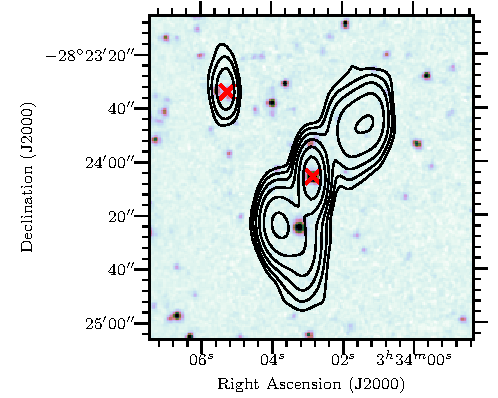
\includegraphics[width=0.6\linewidth]{atlas-images/CI0077C1_fig.pdf}
      \caption[A radio source breaking our assumption that there are no other radio sources with 1~arcmin of the source.]{A $2'$-wide radio image centred on ATLAS3\textunderscore{}J033402.87-282405.8C.
        %
        This radio source breaks the assumption that there are no other radio
        sources within 1~arcmin of the source. Another radio source is visible
        to the upper-left. Host galaxies found by Radio Galaxy Zoo volunteers
        are shown by crosses. {The background image
        is a \unit{3.6}{\micro\meter} image from SWIRE. The contours show ATLAS radio data and start at $4\sigma$, increasing geometrically by a factor of 2.}}
      \label{fig:broken-isolation}
    \end{figure}

    \begin{figure}
      \centering
      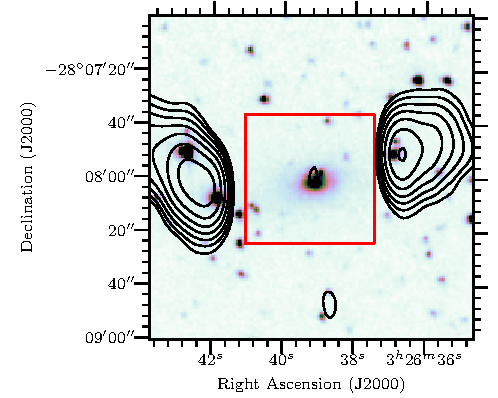
\includegraphics[width=0.6\linewidth]{atlas-images/CI2363_fig.pdf}
      \caption[A radio source where the window centred on the host galaxy does not contain enough radio information to correctly identify the galaxy as a host.]{An example of a radio source where the window centred on the
        host galaxy, shown as a rectangle, does not contain enough radio
        information to correctly identify the galaxy as the host. {The background image
        is a \unit{3.6}{\micro\meter} image from SWIRE. The contours show ATLAS radio data and start at $4\sigma$, increasing geometrically by a factor of 2.}}
      \label{fig:broken-window-size}
    \end{figure}

    \begin{figure}
      \centering
      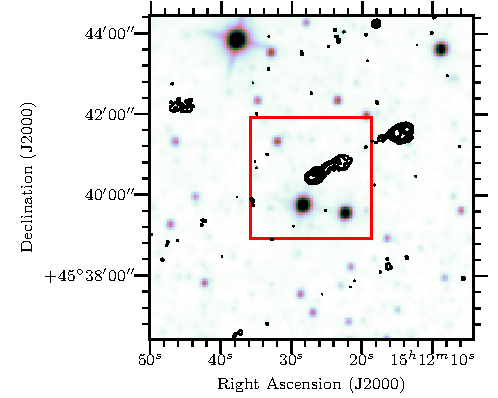
\includegraphics[width=0.6\linewidth]{atlas-images/FIRSTJ151227_fig.pdf}
      \caption[A radio source breaking our assumption that the whole radio source is visible in the chosen radius.]{A $8'$-wide radio image from FIRST, centred on
        FIRST\ J151227.2+454026. The $3'$-wide red box indicates the boundaries of
        the image of this radio component shown to volunteers in Radio Galaxy
        Zoo. This radio source breaks our assumption that the whole radio source
        is visible in the chosen radius. As one of the {components} of the radio source
        is outside of the image, a volunteer (or automated algorithm) looking at
        the $3'$-wide image may be unable to determine that this is a radio
        double or locate the host galaxy. {The background image
        is a \unit{3.4}{\micro\meter} image from \emph{WISE}. The contours show FIRST radio
        data, starting at $4\sigma$ and increasing geometrically by a factor of 2.}}
      \label{fig:broken-contains}
    \end{figure}

    We make a number of assumptions to relate the cross-identification task to
    the candidate classification task:
    \begin{enumerate}
      \item {For any radio component, the $2' \times 2'$ image centred on the component contains components of only one radio source.}
      \item {For any radio component, the $2' \times 2'$ image centred on the component contains all components of this source.}
      \item The host galaxy of a radio component is within the 1~arcmin {search radius around the component, measured from the centre of the Gaussian fit}.
      \item The host galaxy of a radio component is closer on the sky to the
        radio component than the host galaxy of any other radio component.
      \item The host galaxy appears in the SWIRE catalogue.
    \end{enumerate}
    These assumptions limit the effectiveness of our approach, regardless of
    how accurate our binary classifier may be. {Examples of radio sources that break these respective assumptions are:}
    \begin{enumerate}
      \item {A radio source less than $1'$ away from another radio source.}
      \item {A radio source with an angular size greater than $2'$.}
      \item {A radio source with a component greater than $1'$ away from the host galaxy.}
      \item {A two-component radio source with another host galaxy between a component and the true host galaxy.}
      \item {An infrared-faint radio source \citep[as in][]{collier14irfaint}.}
    \end{enumerate}

    {The main limitations are problems of scale in choosing the
    candidate search radius and the size of the windows
    representing candidates. If the search radius is too small, we may not
    consider the host galaxy as a candidate. If the search radius is too
    large, we may consider multiple host galaxies (though this is mostly
    mitigated by the Gaussian weighting). If the window is too small, radio
    emission may extend past the edges of the window and we may miss critical
    information required to identify the galaxy as a host galaxy. If the
    window is too large, then irrelevant information will be included and it
    may be difficult or computationally expensive to score. We choose a
    window size of $32 \times 32$ pixels, corresponding to approximately $48'' \times 48''$ in
    ATLAS. This is shown as squares in \autoref{fig:windows} and
    \autoref{fig:broken-window-size}. These kinds of size problems are
    difficult even for non-automated methods as radio sources can be extremely
    wide---for example, Radio Galaxy Zoo found a radio giant that spanned
    over three different images presented to volunteers and the full source
    was only cross-identified by the efforts of citizen scientists
    \citep{banfield15}. An example of a radio image where part of the radio
    source is outside the search radius is shown in
    \autoref{fig:broken-contains}.}

    In weighting the scores by a Gaussian function of angular
    separation, we implicitly assume that the host galaxy of a radio component
    is closer to that radio component than any other host galaxy. If this
    assumption is not true then the incorrect host galaxy may be identified, though
    this is rare.

    We only need to require that the host galaxy appears in SWIRE to
    incorporate galaxy-specific features
    (\autoref{vector-representation-of-infrared-sources}) and to improve
    efficiency. Our method is applicable even when host galaxies are not detected in
    the infrared by considering every pixel of the radio image as a candidate
    location as would be done in the original computer vision approach. {If the host galaxy location does not correspond to an infrared source, the radio source can be classified as infrared-faint.}

    Our assumptions impose an upper bound on how well we can cross-identify
    radio sources. We estimate this upper bound in \autoref{sec:atlas-xid-cdfs-results}.

  \subsection{Feature vector representation of infrared sources}
  \label{vector-representation-of-infrared-sources}

    {Inputs to binary classifiers must be represented by an array of real values called feature vectors.} We therefore need to choose a feature vector representation of our candidate host galaxies. Candidate hosts are sourced from the SWIRE catalogue (\autoref{sec:atlas-xid-swire}). We represent each candidate host with 1034 real-valued features, {combining the windows centred on each candidate (\autoref{sec:atlas-xid-as-binary-classification}) with ancillary infrared data from the SWIRE catalogue}. For a given candidate host, these features are:
    \begin{itemize}
      \item the 6 base-10 logarithms of the ratios of fluxes of the candidate
        host at the four IRAC wavelengths {(the `colours' of the candidate)};
      \item the flux of the host at \unit{3.6}{\micro\meter};
      \item the stellarity index of the host at both 3.6 and
        \unit{4.5}{\micro\meter};
      \item the radial distance between the candidate host and the nearest
        radio component in the ATLAS catalogue; and
      \item a 32 $\times$ 32 pixel image from ATLAS (approximately $48''
        \times 48''$), centred on the candidate host {(the window)}.
    \end{itemize}

    The infrared colours provide insight into the properties {of the candidate
    host galaxy} \citep{grant11polarised}. The 3.6 and \unit{4.5}{\micro\meter} fluxes trace
    both galaxies with faint polycyclic aromatic hydrocarbon (PAH) emission {(i.e. late-type, usually star-forming galaxies)}
    and elliptical galaxies dominated by old stellar populations. The
    \unit{5.8}{\micro\meter} flux selects galaxies where the infrared emission
    is dominated by non-equilibrium emission of dust grains {due to active galactic nuclei},
    while the \unit{8.0}{\micro\meter} flux
    traces strong PAH emission at low redshift \citep{sajina2005}. The
    stellarity index {is a value in the SWIRE catalogue that represents how likely the object is to be a star rather
    than a galaxy \citep{surace05swire}. It was estimated by a neural network in
    \texttt{SExtractor} \citep{bertin96sextractor}}.

    We use the $32 \times 32$ pixels of each radio window as independent
    features for all binary classification models, with the convolutional neural
    network automatically extracting features that are relevant. Other
    features of the radio components may be used instead of just relying on the pixel values,
    but there has been limited research on extracting such features:
    \citet{proctor06} describes hand-selected features for radio doubles in
    FIRST, and \citet{aniyan17cnn} and \citet{lukic18compact} make use of
    deep convolutional neural networks which automatically extract features as
    part of classification. A more comprehensive investigation of features is
    a good avenue for potential improvement in our pipeline but this is beyond
    the scope of this initial study.

  \subsection{Binary classifiers}\label{sec:atlas-xid-classifiers}

    We use three different binary classification models: logistic regression,
    convolutional neural networks, and random forests. These models cover
    three different approaches to machine learning. Logistic regression is a
    probabilistic binary classification model. It is linear in the feature
    space and outputs the probability that the input has a positive
    label~\citep[Chap. 4]{bishop06ml}. Convolutional neural networks (CNN) are
    biologically inspired prediction models with image inputs.
    They have recently produced good results on large image-based datasets in
    astronomy \citep[e.g.]{lukic18compact, dieleman15cnn}. Random
    forests are an ensemble of decision trees~\citep{breiman01random-forest}.
    They consider multiple subsamples of the training set, where each
    bootstrap subsample is sampled with replacement from the training set. To
    classify a new data point, the random forest takes the weighted average of
    all classifications produced by each decision tree. For a more detailed description of these models, see \aref{sec:atlas-xid-models}.

  \subsection{Labels}\label{sec:atlas-xid-labels}

    \begin{figure}
      \centering
      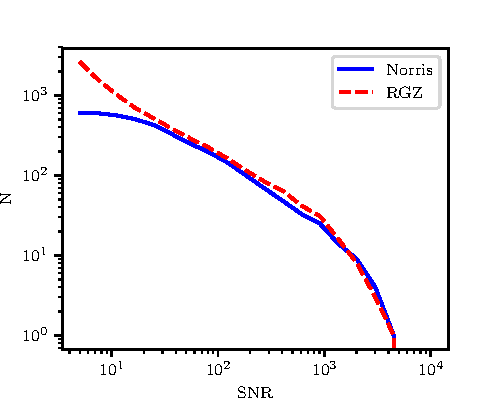
\includegraphics[width=0.6\columnwidth]{atlas-images/snr_cutoff_cumulative.pdf}
      \caption[Cumulative number of radio components in the expert and Radio Galaxy
        Zoo training sets with different signal-to-noise ratios.]{Cumulative number of radio components ($N$) in the expert (Norris) and Radio Galaxy
        Zoo (RGZ) training sets with different signal-to-noise ratios (SNR).}
      \label{fig:distribution-cutoffs}
    \end{figure}

    \begin{figure}
      \centering
      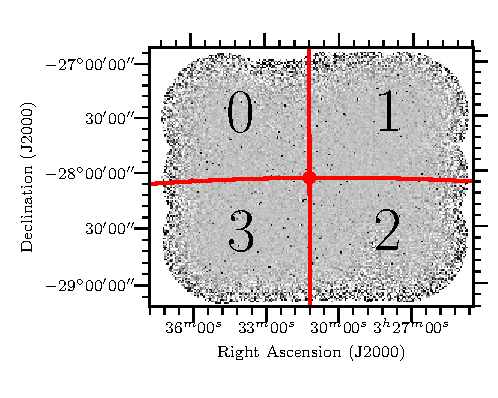
\includegraphics[width=0.6\columnwidth, trim={0cm 0.5cm 0cm 0.5cm}, clip]{atlas-images/quadrants.pdf}
      \caption[CDFS field training and testing quadrants.]{CDFS field training and testing quadrants labelled 0 -- 3. The
        central dot is located at $\alpha = 03^\text{h}31^\text{m}12^\text{s},
        \delta = -28^\circ{}06'00''$. The quadrants are chosen such that
        there are similar numbers of radio sources in each
        quadrant.\label{fig:quadrants}}
    \end{figure}

    \begin{table}
      \caption[Number of compact and resolved radio objects in each CDFS
      quadrant.]{Number of compact and resolved radio objects in each CDFS
      quadrant. Radio Galaxy Zoo (RGZ) has more cross-identifications than the
      expert catalogue \citep{norris06} provides as it uses a deeper data release of ATLAS, and
      so has more objects in each quadrant for training.}
      \label{tab:radio-count}
      \centering
      \begin{tabular}{lcccc}
        \hline\hline
        Quadrant & Compact & Resolved & Compact & Resolved\\
        &&&(RGZ)&(RGZ)\\
        \hline
        0 & 126 & 24 & 410 & 43 \\
        1 & 99 & 21 & 659 & 54 \\
        2 & 61 & 24 & 555 & 57 \\
        3 & 95 & 18 & 631 & 51 \\
        \hline
        \textit{Total} & 381 & 87 & 2255 & 205\\
        \hline\hline
      \end{tabular}
    \end{table}

    {The Radio Galaxy Zoo and \citet{norris06} cross-identification
    catalogues must be converted to binary labels for infrared objects so that
    they can be used to train binary classifiers. There are two challenges with this conversion:
    \begin{itemize}
      \item We can only say that an object is \emph{a} host galaxy, not which radio object it is associated with, and
      \item We cannot disambiguate between non-host infrared objects and host galaxies that are not in the cross-identification catalogue.
    \end{itemize}
    
    We use the Gaussian weighting described in \autoref{sec:atlas-xid-as-binary-classification} to address the first issue.
    The second issue is known as a `positive-unlabelled' classification problem, which is
    a binary classification problem where we only observe labels for the
    positive class. We treat unlabelled objects as negative examples following
    \citet{menon15cpe}. That is, we make the na\"ive assumption that any
    infrared object in the SWIRE catalogue not identified as a host galaxy in a cross-identification catalogue is not a host galaxy at all.}

    We first generate positive labels from a cross-identification catalogue.
    We decide that if an infrared object is listed in the catalogue, then it
    is assigned a positive label as a host galaxy. We then assign every other galaxy a negative label. This has some problems---an example is that if the cross-identification catalogue does not include a radio
    object (e.g.~it is below the signal-to-noise ratio) then the host galaxy
    of that radio object receives a negative label. This occurs with
    \citet{norris06} cross-identifications, as these are associated with the
    first data release of ATLAS. The first data release went to a 5$\sigma$
    flux density level of $S_{1.4} \geq \unit{200}{\micro\jansky}\text{
    beam}^{-1}$ \citep{norris06}, compared to $S_{1.4} \geq \unit{85}{\micro\jansky}\text{
    beam}^{-1}$ for the third data release used by Radio Galaxy Zoo
    \citep{franzen15}. The labels from \citet{norris06} may therefore disagree with labels
    from Radio Galaxy Zoo even if they are both plausible. The difference in
    training set size at different flux cutoffs is shown in
    \autoref{fig:distribution-cutoffs}. We train and test our binary
    classifiers on infrared objects within a 1~arcmin radius of an ATLAS radio
    component.

  \subsection{Experimental setup}
  \label{sec:atlas-xid-experimental-setup}

    We trained binary classifiers on infrared objects in the CDFS field using
    two sets of labels. One label set was derived from Radio Galaxy Zoo
    cross-identifications and the other was derived from the \citet{norris06}
    cross-identification catalogue. We refer to these as the `Radio Galaxy Zoo
    labels' and the `expert labels' respectively. We divided the CDFS field
    into four quadrants for training and testing. The quadrants were divided
    with a common corner at $\alpha = 03^\text{h}31^\text{m}12^\text{s},
    \delta = -28^\circ{}06'00''$ as shown in \autoref{fig:quadrants}. For
    each trial, one quadrant was used to extract test examples and the other
    three quadrants were used for training examples.

    We further divided the radio components into compact and resolved. Compact
    components are cross-identified by fitting a 2D Gaussian \citep[as
    in][]{norris06} and we would expect any machine learning approach for host
    cross-identification to attain high accuracy on this set. A radio component was
    considered resolved if
    \begin{equation}
      \label{eq:atlas-compact}
        \ln \left(
          \frac{S_{\text{int}}}
               {S_{\text{peak}}}
        \right) > 2\sqrt{\left(
          \frac{\sigma_{S_{\text{int}}}}
               {S_{\text{int}}}
        \right)^2 + \left(
          \frac{\sigma_{S_{\text{peak}}}}
               {S_{\text{peak}}}
        \right)^2}\,\,\,\,,
    \end{equation}%
    where \(S_{\text{int}}\) is the integrated flux density,
    \(S_{\text{peak}}\) is the peak flux density, {$\sigma_{S_{\text{int}}}$ is
    the uncertainty in integrated flux density and $\sigma_{S_{\text{peak}}}$
    is the uncertainty in peak flux density} \citep[following][]{franzen15}.

    Candidate hosts were selected from the SWIRE catalogue. For a given subset
    of radio components, all SWIRE objects within 1~arcmin of all radio
    components in the subset were added to the associated SWIRE subset. In results
    for the candidate classification task, we refer to SWIRE objects
    within 1~arcmin of a compact radio component as part of the `compact set',
    and SWIRE objects within 1~arcmin of a resolved radio component as part of
    the `resolved set'.

    To reduce bias in the testing data due to the expert labels being
    generated from a shallower data release of ATLAS, a SWIRE object was only
    included in the test set if it was within 1~arcmin of a radio object with
    a SWIRE cross-identification in both the \citet{norris06} catalogue and the
    Radio Galaxy Zoo catalogue.

    Each binary classifier was trained on the training examples and used to
    {score the test examples. These scores were thresholded to generate labels which could be directly compared
    to the expert labels. We then computed the `balanced accuracy' of these predicted labels.} Balanced
    accuracy is the average of the accuracy on the positive class and the
    accuracy on the negative class, and is not sensitive to class imbalance.
    The candidate classification task has highly imbalanced classes---in our
    total set of SWIRE objects within 1~arcmin of an ATLAS object, only 4 per
    cent have positive labels. {Our threshold was chosen to maximise the balanced
    accuracy on predicted labels of the training set.} Only examples within 1~arcmin of ATLAS objects
    in the first ATLAS data release \citep{norris06} were used to compute
    balanced accuracy, as these were the only ATLAS objects with expert labels.

    We then used the scores to predict the host galaxy
    for each radio component cross-identified by both \citet{norris06} and
    Radio Galaxy Zoo. {We followed \autoref{alg:xid}:
    The score of each SWIRE object within 1~arcmin of a given radio
    component was weighted by a Gaussian function of angular separation from the
    radio component and the object with the highest
    weighted score was chosen as the host galaxy.} The
    {cross-identification accuracy} was then estimated as the
    fraction of the predicted host galaxies that matched the \citet{norris06}
    cross-identifications.

\section{Results}\label{sec:atlas-xid-results}

  In this section we present accuracies of our method trained on CDFS and
  applied to CDFS and ELAIS-S1, as well as results motivating our accuracy
  measures and estimates of upper and lower bounds for cross-identification
  accuracy using our method.

  \subsection{Application to ATLAS-CDFS}
  \label{sec:atlas-xid-cdfs-results}

    \begin{figure}
      \centering
      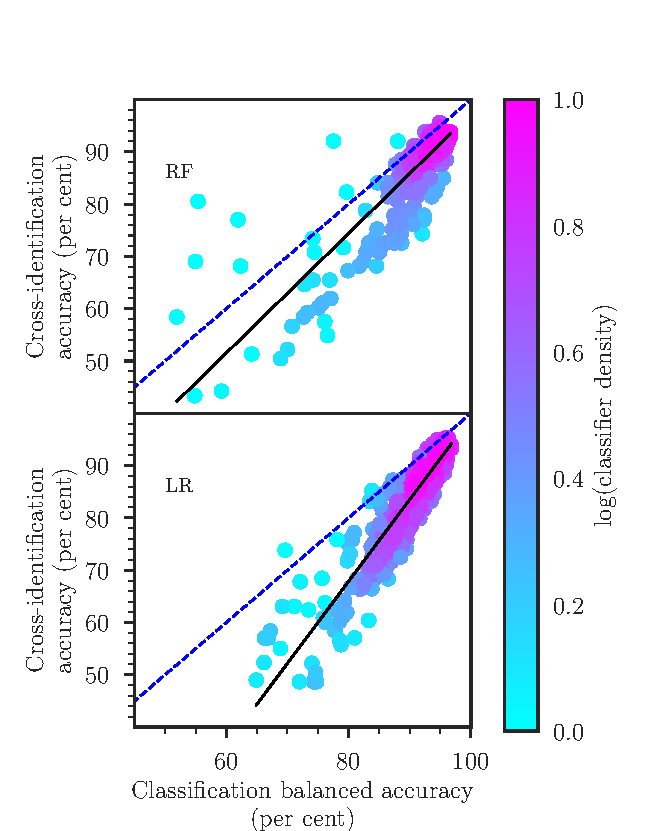
\includegraphics[width=0.6\columnwidth]{atlas-images/gct-to-xid.pdf}
      \caption[Balanced accuracy on the candidate classification task plotted
      against accuracy on the cross-identification task.]{Balanced accuracy on the candidate classification task plotted
      against accuracy on the cross-identification task. `RF' indicates
      results from random forests, and `LR' indicates results from logistic
      regression. Binary classifiers were trained on random, small subsets of the
      training data to artificially restrict their accuracies. Colour shows
      the density of points on the plot estimated by a Gaussian kernel density
      estimate. The solid lines indicate the best linear fit; these fits have
      $R^2 = 0.92$ for logistic regression and $R^2 = 0.87$ for random
      forests.
      {The dashed line shows the line where cross-identification accuracy and candidate classification accuracy are equal.}
      We did not include convolutional neural networks in this test,
      as training them is very computationally expensive. There are 640 trials shown per classification model. These results
      exclude binary classifiers with balanced accuracies less than 51 per cent, as
      these are essentially random.
      \label{fig:gct-to-xid}}
    \end{figure}

    \begin{figure}
      \centering
      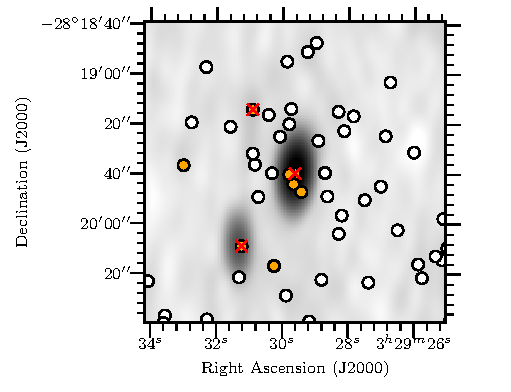
\includegraphics[width=0.6\columnwidth]{atlas-images/positives.pdf}
      \caption[An example of predicted host galaxies in the candidate classification task.]{Predicted host galaxies in the candidate classification task for ATLAS3~J032929.61-281938.9. {The background image is an ATLAS radio image.} Radio Galaxy Zoo host galaxies
      are marked by crosses. SWIRE candidate host galaxies are circles coloured by {the score output by a logistic regression binary classifier. The scores are thresholded to obtain labels, as when we compute balanced accuracy.} Orange circles have been assigned a `positive' label by a logistic regression binary classifier and white otherwise. {Note that there are more predicted host galaxies than there are radio components, so not all of the predicted host galaxies would be assigned as host galaxies in the cross-identification task.}
      \label{fig:positives}}
    \end{figure}

    \begin{figure*}
    \centering
    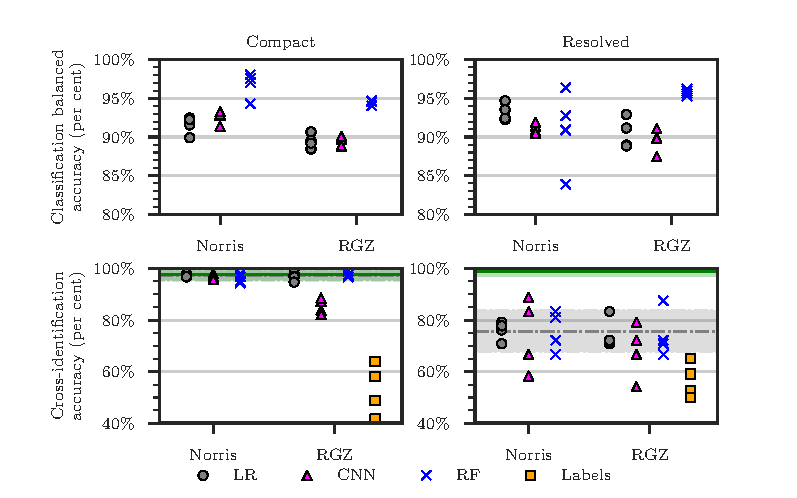
\includegraphics[width=1.0\linewidth]{atlas-images/cdfs-grid-new.pdf}
    \caption[Performance of our method with different binary classifiers on the binary classification task.]{Performance of our method with logistic regression (`LR'), convolutional neural networks (`CNN') and random forest (`RF') binary classifiers. `Norris' indicates the performance of binary classifiers trained on the expert labels and `RGZ' indicates the performance of binary classifiers trained on the Radio Galaxy Zoo labels. One point is shown per binary classifier per testing quadrant. The training and testing sets have been split into compact (left) and resolved (right) objects. {Shown for comparison is the accuracy of the Radio Galaxy Zoo consensus cross-identifications on the cross-identification task, shown as `Labels'.} The cross-identification accuracy attained by a perfect binary classifier is shown by a solid green line, and the cross-identification accuracy of a nearest neighbours approach is shown by a dashed grey line. The standard deviation of these accuracies across the four CDFS quadrants is shown by the shaded area. Note that the pipeline shown in \autoref{fig:flowchart} is not used for these results. \label{fig:ba}}
    \end{figure*}

    \begin{figure}
      \centering
      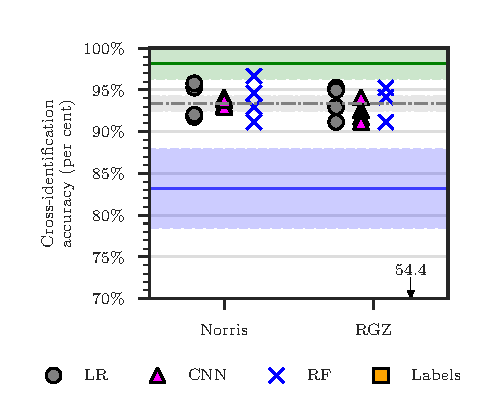
\includegraphics[]{atlas-images/cdfs_cross_identification_grid.pdf}
      \caption[Performance of our approach using different binary classifiers on the cross-identification task.]{Performance of our approach using different binary classifiers on the cross-identification task. Markers and lines are as in \autoref{fig:ba}. The blue solid line indicates the performance of a random binary classifier and represents the minimum accuracy we expect to obtain. The standard deviation of this accuracy across 25 trials and 4 quadrants is shaded. The accuracy of Radio Galaxy Zoo on the cross-identification task is below the axis and is instead marked by an arrow with the mean accuracy. Note that the pipeline shown in \autoref{fig:flowchart} is used here, {so compact objects are cross-identified in the same way regardless of binary classifier model}. \label{fig:cross-id-accuracy}}
    \end{figure}

    {We can assess trained binary classifiers either by their performance on
    the candidate classification task or by their performance on the
    cross-identification task when used in our method. Both performances are
    useful: Performance on the candidate classification task provides a robust
    and simple way to compare binary classifiers without the limitations of
    our specific formulation, and performance on the cross-identification task
    can be compared with other cross-identification methods. We therefore
    report two sets of accuracies: balanced accuracy for the galaxy
    classification task and accuracy for the cross-identification task. These
    accuracy measures are correlated and we show this correlation in
    \autoref{fig:gct-to-xid}. Fitting a line of best fit with \texttt{scipy}
    gives $R^2 = 0.92$ for logistic regression and $R^2 = 0.87$ for random
    forests. While performance on the candidate classification task is correlated
    with performance on the cross-identification task, balanced accuracy does
    not completely capture the effectiveness of a binary classifier applied to
    the cross-identification task. {This is because while our binary
    classifiers output real-valued scores, these scores are thresholded to
    compute the balanced accuracy}. In the candidate classification
    task, the binary classifier only needs to ensure that host galaxies are
    {scored higher} than non-host galaxies. This means
    {that after thresholding} there can be
    many `false positives' that do not affect cross-identification. An example
    of this is shown in \autoref{fig:positives}, where the classifier has
    identified eight `host galaxies'. However, there are only three true host
    galaxies in this image---one per radio component---and so in the
    cross-identification task, only three of these galaxies will be identified
    as hosts.}

    In \autoref{fig:ba} we plot {the balanced accuracies of our classification models
    on the candidate classification task and the cross-identification
    accuracies of our method using each of these models. Results are shown for both
    the resolved and compact sets.} For comparison, we also plot the cross-identification accuracy of Radio Galaxy
    Zoo and a nearest neighbours approach, as well as estimates for upper and
    lower limits on the cross-identification accuracy. {We estimate the upper limit on performance by assigning all
    true host galaxies a score of 1 and
    assigning all other candidate host galaxies a score of 0. This
    is equivalent to `perfectly' solving the candidate classification task and so
    represents the best possible cross-identification performance achievable
    with our method. We estimate the lower limit on performance by {
    assigning random scores to each candidate host galaxy}. We expect any
    useful binary classifier to produce better
    results than this, so this represents the lowest expected
    cross-identification performance.} The upper estimates, lower estimates,
    and nearest neighbour accuracy are shown as horizontal lines in
    \autoref{fig:ba}.

    In \autoref{fig:cross-id-accuracy} we plot the performance {of our
    method using different binary classification models}, as well as the
    performance of Radio Galaxy Zoo, nearest neighbours, and the perfect and
    random binary classifiers on the full set of ATLAS~DR1 radio components
    using the pipeline in \autoref{fig:flowchart}. The accuracy
    {associated with each classification model} and training label set
    averaged across all four quadrants is shown in \aref{sec:atlas-xid-accuracies}.

    Differences between accuracies across training labels are well within one
    standard deviation computed across the four quadrants, with convolutional
    neural networks on compact objects as the only exception. The spread of
    accuracies is similar for both sets of training labels, with the exception
    of random forests. The balanced accuracies of random forests trained on
    expert labels have a considerably higher spread than those trained on
    Radio Galaxy Zoo labels, likely because of the small size of the expert
    training set---there are less than half the number of objects in the
    expert-labelled training set than the number of objects in the Radio
    Galaxy Zoo-labelled training set (\autoref{tab:radio-count}).

    Radio Galaxy Zoo-trained methods significantly outperform Radio Galaxy Zoo
    cross-identifications. Additionally, despite poor performance of Radio
    Galaxy Zoo on the cross-identification task, methods trained on these
    cross-identifications still perform comparably to those trained on expert
    labels. This is because incorrect Radio Galaxy Zoo cross-identifications
    can be thought of as a source of noise in the labels which is `averaged out'
    in training. This shows the usefulness of crowdsourced training data, even
    when the data is noisy.

    Our method performs comparably to a nearest neighbours approach. For
    compact objects, this is to be expected---indeed, nearest neighbours
    attains nearly 100 per cent accuracy on the compact test set. Our results
    do not improve on nearest neighbours for resolved objects. However, our
    method does allow for improvement on nearest neighbours with a
    sufficiently good binary classifier: A `perfect' binary classifier attains
    nearly 100 per cent accuracy on resolved sources. This shows that our
    method may be useful provided that a good binary classifier can be
    trained. The most obvious place for improvement is in feature selection:
    We use pixels of radio images directly and these are likely not conducive
    to good performance on the candidate classification task. Convolutional
    neural networks, which are able to extract features from images,
    \emph{should} work better, but these require far more training data than
    the other methods that we applied and the small size of ATLAS thus limits their performance.

    We noted in \autoref{sec:atlas-xid-labels} that the test set of expert labels,
    derived from the initial ATLAS data release, was less deep than the third
    data release used by Radio Galaxy Zoo and this chapter, introducing a source
    of label noise in the testing labels. Specifically, true host galaxies may
    be misidentified as non-host galaxies if the associated radio source is
    below the 5 signal-to-noise limit in ATLAS~DR1 but not in ATLAS~DR3. This
    has the effect of reducing the accuracy for Radio Galaxy Zoo-trained
    classifiers.

    {We report the scores predicted by each classifier for each
    SWIRE object in \aref{sec:atlas-xid-scores} and the predicted
    cross-identification for each ATLAS object in \aref{sec:atlas-xid-xids}.
    Scores we report for a given object were predicted by binary
    classifiers tested on the quadrant containing that object. The reported scores are not weighted.}

    In \autoref{fig:examples} we show five resolved sources where the most classifiers disagreed on the correct cross-identification.

\subsection{Application to ATLAS-ELAIS-S1}
  \label{sec:atlas-xid-elais}

  \begin{figure*}
  \centering
  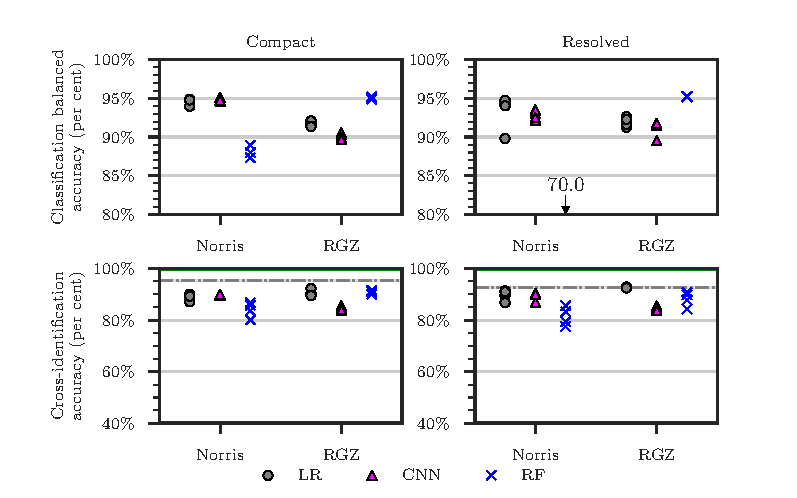
\includegraphics[]{atlas-images/elais-grid-new.pdf}
  \caption[Performance of different classification models on the binary classification task, tested on ELAIS-S1.]{Performance of different classification models trained on CDFS and tested on
  resolved and compact sources in ELAIS-S1. Points represent classification models
  trained on different quadrants of CDFS, with markers, lines, and axes as in
  \autoref{fig:ba}. The balanced acccuracy of expert-trained random forest
  binary classifiers falls below the axis and the corresponding mean accuracy is
  shown by an arrow. The estimated best attainable accuracy is almost 100 per cent.
    \label{fig:elais-ba}}
  \end{figure*}

  \begin{figure}
    \centering
    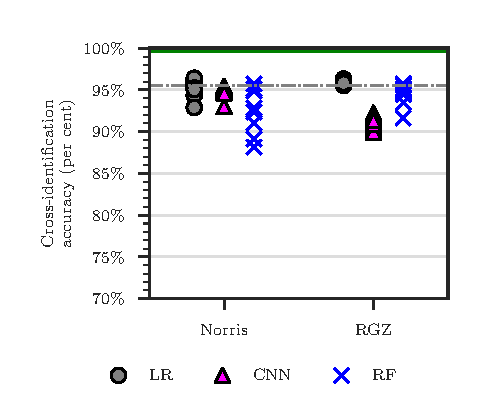
\includegraphics[]{atlas-images/elais_cross_identification_grid.pdf}
    \caption[Performance of different classification models on the cross-identification task, tested on ELAIS-S1.]{Performance of different classifiers trained on CDFS and tested
    on ELAIS-S1. Markers are as in \autoref{fig:cross-id-accuracy} and
    horizontal lines are as in \autoref{fig:elais-ba}. Note that the pipeline
    shown in \autoref{fig:flowchart} is used here, {so compact objects
    are cross-identified in the same way regardless of binary classifier
    model}.
      \label{fig:elais-cross-id-accuracy}}
  \end{figure}

  \begin{figure}
    \centering
    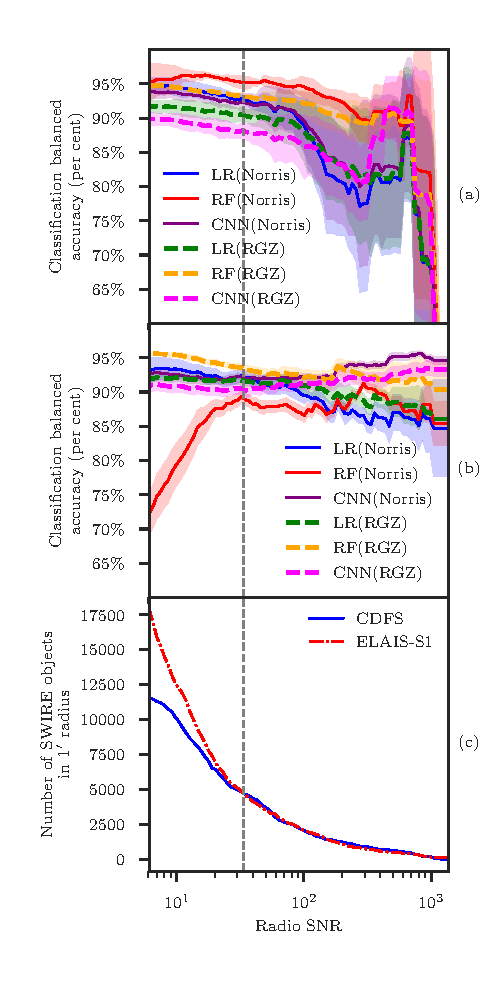
\includegraphics[trim={0cm 1cm 0cm 0.5cm}, clip]{atlas-images/accuracies-flux-snr.pdf}
    \caption[Balanced accuracies of classifiers with different SNR cutoffs.]{(a) Balanced accuracies of classifiers trained and tested on CDFS
      with different signal-to-noise ratio (SNR) cutoffs for the test set. A
      SWIRE object is included in the test set if it is within $1'$ of a radio
      component with greater SNR than the cutoff. Lines of different colour
      indicate different classifier/training labels combinations, where LR is
      logistic regression, RF is random forests, CNN is convolutional neural
      networks, and Norris and RGZ are the expert and Radio Galaxy Zoo label
      sets respectively. Filled areas represent standard deviations across
      CDFS quadrants. (b) Balanced accuracies of classifiers trained on CDFS
      and tested on ELAIS-S1. (c) A cumulative distribution plot of SWIRE
      objects associated with a radio object with greater SNR than the cutoff.
      The grey dashed line shows the SNR level at which the number of SWIRE
      objects above the cutoff is equal for CDFS and ELAIS-S1. This cutoff level
      is approximately at a SNR of $34$.}
    \label{fig:accuracies-flux}
  \end{figure}

  We applied the method trained on CDFS to perform cross-identification on the
  ELAIS-S1 field. Both CDFS and ELAIS-S1 were imaged by the same radio
  telescope to similar sensitivities and angular resolution for the ATLAS
  survey. {We can use the SWIRE cross-identifications made by
  \citet{middelberg08} to derive another set of expert labels, and hence
  determine how accurate our method is. If our method generalises well across
  different parts of the sky, then we expect CDFS-trained classifiers to have
  comparable performance between ELAIS-S1 and CDFS}. In \autoref{fig:elais-ba}
  we plot the performance of CDFS-trained classification models on the candidate classification task and
  the performance of our method on the cross-identification task using these models. We also plot
  the cross-identification accuracy of a nearest neighbours approach\footnote{{We cannot
  directly compare our method applied to ELAIS-S1 with Radio Galaxy Zoo, as
  Radio Galaxy Zoo does not include ELAIS-S1.}}. In
  \autoref{fig:elais-cross-id-accuracy} we plot the performance of our method
  on the full set of ELAIS-S1 ATLAS~DR1 radio components using the pipeline in
  \autoref{fig:flowchart}. We list the corresponding accuracies in
  \aref{sec:atlas-xid-accuracies}.

  Cross-identification results from ELAIS-S1 are similar to those for CDFS,
  showing that our method trained on CDFS performs comparably well on
  ELAIS-S1. However, nearest neighbours outperforms most methods on ELAIS-S1.
  This is likely because there is a much higher percentage of compact objects
  in ELAIS-S1 than in CDFS. The maximum achievable accuracy we have estimated
  for ELAIS-S1 is very close to 100 per cent, so (as for CDFS) a very accurate
  binary classifier would outperform nearest neighbours.

  One interesting difference between the ATLAS fields is that random forests
  trained on expert labels perform well on CDFS but poorly on ELAIS-S1. This
  is not the case for logistic regression or convolutional neural networks
  trained on expert labels, nor is it the case for random forests trained on
  Radio Galaxy Zoo. We hypothesise that this is because the ELAIS-S1
  cross-identification catalogue \citep{middelberg08} labelled fainter radio
  components than the CDFS cross-identification catalogue \citep{norris06} due
  to noise from the very bright source
  ATCDFS\textunderscore{}J032836.53-284156.0 in CDFS. Classifiers trained on
  CDFS expert labels may thus be biased toward brighter radio components
  compared to ELAIS-S1. Radio Galaxy Zoo uses a preliminary version of the third data release of ATLAS
  \citep{franzen15} and so classifiers trained on the Radio Galaxy Zoo labels
  may be less biased toward brighter sources compared to those trained on the
  expert labels. To test this hypothesis we tested each classification model against
  test sets with a signal-to-noise ratio (SNR) cutoff. A SWIRE object was only
  included in the test set for a given cutoff if it was located within $1'$ of
  a radio component with a SNR above the cutoff. The balanced accuracies for
  each classifier at each cutoff are shown in \autoref{fig:accuracies-flux}(a)
  and (b) and the distribution of test set size for each cutoff is shown in
  \autoref{fig:accuracies-flux}(c). \autoref{fig:accuracies-flux}(c) shows
  that ELAIS-S1 indeed has more faint objects in its test set than the CDFS test set, with the SNR for
  which the two fields reach the same test set size (approximately $34$)
  indicated by the dashed vertical line on each plot. For CDFS, all
  classifiers perform reasonably well across cutoffs, with performance
  dropping as the size of the test set becomes small. For ELAIS-S1, logistic
  regression and convolutional neural networks perform comparably across all
  SNR cutoffs, but random forests do not. While random forests trained on
  Radio Galaxy Zoo labels perform comparably to other classifiers across all
  SNR cutoffs, random forests trained on expert labels show a considerable
  drop in performance below the dashed line.

\section{Discussion}

  {Based on the ATLAS sample}, our main result is that it is possible
  to cast radio host galaxy cross-identification as a machine learning task
  for which standard methods can be applied. These methods can then be trained
  with a variety of label sets derived from cross-identification catalogues.
  While our methods have not outperformed nearest neighbours, we have demonstrated that
  for a very accurate binary classifier, good cross-identification results can
  be obtained using our method. Future work could combine multiple catalogues
  or physical priors to boost performance.

  Nearest neighbours approaches outperform most methods we investigated,
  notably including Radio Galaxy Zoo. This is due to the large number of
  compact or partially resolved objects in ATLAS. This result shows that for
  compact and partially resolved objects, methods that do not use machine
  learning such as a nearest neighbours approach or likelihood ratio
  \citep{weston18lrpy} should be preferred to machine learning methods. It
  also shows that ATLAS is not an ideal dataset for developing machine
  learning methods like ours. Our use of ATLAS is motivated by its status as a
  pilot survey for EMU, so methods developed for ATLAS should also work for
  EMU. New methods developed should work well with extended radio sources, but
  this goal is almost unsupported by ATLAS as it has very few examples of such
  sources. This makes both training and testing difficult---there are too
  few extended sources to train on and performance on such a small test set
  may be unreliable. Larger datasets with many extended sources like FIRST
  exist, but these are considerably less deep than and at a different
  resolution to EMU, so there is no reason to expect methods trained on such
  datasets to be applicable to EMU.

  The accuracies of our trained cross-identification methods generally fall
  far below the estimated best possible accuracy attainable using our approach,
  indicated by the green-shaded areas in Figures \ref{fig:cross-id-accuracy} and
  \ref{fig:elais-cross-id-accuracy}. The balanced accuracies attained by our
  binary classifiers indicate that there is significant room for improvement
  in classification. The classification accuracy could be improved by better
  model selection and more training data, particularly for convolutional
  neural networks. There is a huge variety of ways to build a convolutional
  neural network, and we have only investigated one architecture. For an
  exploration of different convolutional neural network architectures applied
  to radio astronomy, see \citet{lukic18compact}. Convolutional neural
  networks generally require more training data than other machine learning
  models and we have only trained our networks on a few hundred sources. We
  would expect performance on the classification task to greatly increase
  with larger training sets.

  Another problem is that of the window size used to select radio features.
  Increasing window size would increase computational expense, but provide
  more information to the models. Results are also highly sensitive to how
  large the window size is compared to the size of the radio source we are
  trying to cross-identify, with large angular sizes requiring large window
  sizes to ensure that the features contain all the information needed to
  localise the host galaxy. An ideal implementation of our method would most
  likely represent a galaxy using radio images taken at multiple window
  sizes, but this is considerably more expensive.

  Larger training sets, better model selection, and larger window sizes would
  improve performance, but only so far: We would still be bounded above by the
  estimated `perfect' classifier accuracy. From this point, the performance
  can only be improved by addressing our broken assumptions. We detailed
  these assumptions in \autoref{sec:atlas-xid-limitations}, and we will discuss here how
  {our method could be adapted to avoid these assumptions}. Our assumption that the host galaxy is contained
  within the search radius could be improved by dynamically choosing the
  search radius, perhaps based on the angular extent of the radio emission, or the
  redshift of candidate hosts. Radio morphology information may allow us to
  select relevant radio data and hence relax the assumption that a $1'$-wide
  radio image represents just one, whole radio source. Finally, our assumption
  that the host galaxy is detefcted in infrared is technically not needed, as
  the sliding-window approach we have employed will still work even if there
  are no detected host galaxies---instead of classifying candidate hosts,
  simply classify each pixel in the radio image. The downside of removing
  candidate hosts is that we are no longer able to reliably incorporate host
  galaxy information such as colour and redshift, though this could be
  resolved by treating pixels as potentially undetected candidate hosts with
  noisy features.

  We observe that Radio Galaxy Zoo-trained methods perform comparably to
  methods trained on expert labels. This shows that the crowdsourced labels
  from Radio Galaxy Zoo will provide a valuable source of training
  data for future machine learning methods in radio astronomy.

  Compared to nearest neighbours, cross-identification accuracy on ELAIS-S1 is
  lower than on CDFS. Particularly notable is that our performance on compact
  objects is very low for ELAIS-S1, while it was near-optimal for CDFS. These
  differences may be for a number of reasons. ELAIS-S1 has beam size and noise
  profile different from CDFS (even though both were imaged with the same
  telescope), so it is possible that our methods over-adapted to the beam and
  noise of CDFS. Additionally, CDFS contains a very bright source which may
  have caused artefacts throughout the field that are not present in ELAIS-S1.
  Further work is required to understand the differences between the fields
  and their effect on performance.

  \autoref{fig:accuracies-flux} reveals interesting behaviour of different
  classifier models at different flux cutoffs. Logistic regression and
  convolutional neural networks seem relatively independent of flux, with
  these models performing well on the fainter ELAIS-S1 components even when
  they were trained on the generally brighter components in CDFS. Conversely,
  random forests were sensitive to the changes in flux distribution between
  datasets. This shows that not all models behave similarly on radio data,
  and it is therefore important to investigate multiple models when
  developing machine learning methods for radio astronomy.

  {\aref{sec:atlas-xid-examples} (see \autoref{fig:examples}) shows examples of incorrectly cross-identified
  components in CDFS. On no such component do all classifiers agree.
  This raises the possibility of using the level of disagreement of an
  ensemble of binary classifiers as a measure of the difficulty of cross-identifying a radio component,
  analogous to the consensus level for Radio Galaxy Zoo volunteers.}

  Our methods can be easily incorporated into other cross-identification
  methods or used as an extra data source for source detection. For
  example, the scores output by our binary classifiers could be used to
  disambiguate between candidate host
  galaxies selected by model-based algorithms, or used to weight candidate
  host galaxies while a source detector attempts to associate radio
  components. Our method can also be extended using other data sources: For
  example, information from source identification algorithms could be
  incorporated into the feature set of candidate host galaxies.

\section{Summary}

  We presented a machine learning approach for cross-identification of radio
  components with their corresponding infrared host galaxies. Using the CDFS
  field of ATLAS as a training set we trained our
  methods on expert and crowdsourced cross-identification catalogues.
  Applying these methods on both fields of ATLAS, we found that:
  \begin{itemize}
    \item Our method trained on ATLAS observations of CDFS generalised to
    ATLAS observations of ELAIS-S1, demonstrating that training on a single
    patch of sky is a feasible option for training machine learning methods
    for wide-area radio surveys;
    \item Performance was comparable to nearest neighbours even on resolved
    sources, showing that nearest neighbours is useful for datasets consisting
    mostly of unresolved sources such as ATLAS and EMU;
    \item Radio Galaxy Zoo-trained models performed comparably to
    expert-trained models and outperformed Radio Galaxy Zoo, showing that
    crowdsourced labels are useful for training machine learning methods for
    cross-identification even when these labels are noisy;
    \item ATLAS does not contain sufficient data to train or test machine
    learning cross-identification methods for extended radio sources. This
    suggests that if machine learning methods are to be used on EMU, a larger
    area of sky will be required for training and testing these methods.
    However, existing surveys like FIRST are likely too different from EMU to expect
    good generalisation.
  \end{itemize}

  While our cross-identification performance is not as high as desired, we
  make no assumptions on the binary classification model used in our methods
  and so we expect the performance to be improved by further experimentation
  and model selection. Our method provides a useful framework for generalising
  cross-identification catalogues to other areas of the sky from the same
  radio survey and can be incorporated into existing methods. {We have
  shown that citizen science can provide a useful dataset for training machine
  learning methods in the radio domain.} \autoref{cha:rlfs} will extend this
  approach and confirm that dataset size is a key limitation by successfully applying it to a considerably larger dataset: FIRST.

\section{Acknowledgements}

  This chapter and corresponding publication was made possible by the participation of more than
  11~000 volunteers in the Radio Galaxy Zoo project. Their contributions are
  individually acknowledged at \url{http://rgzauthors.galaxyzoo.org}. Parts of
  this research were conducted by the Australian Research Council Centre of
  Excellence for All-sky Astrophysics (CAASTRO), through project number
  CE110001020. Partial support for LR was provided by U.S. National Science
  Foundation grants AST1211595 and 1714205 to the University of Minnesota. HA
  benefitted from grant 980/2016-2017 of Universidad de Guanajuato. We thank
  A.~Tran and the anonymous referee for their comments on the manuscript this chapter was based on.
  Radio Galaxy Zoo makes use of
  data products from the Wide-field Infrared Survey Explorer and the Very
  Large Array. The Wide-field Infrared Survey Explorer is a joint project of
  the University of California, Los Angeles, and the Jet Propulsion
  Laboratory/California Institute of Technology, funded by the National
  Aeronautics and Space Administration. The National Radio Astronomy
  Observatory is a facility of the National Science Foundation operated under
  cooperative agreement by Associated Universities, Inc. The figures
  in this work make use of Astropy, a community-developed core Python package
  for Astronomy \citep{astropy}. The Australia Telescope Compact Array is part
  of the Australia Telescope, which is funded by the Commonwealth of Australia
  for operation as a National Facility managed by CSIRO. We acknowledge the Gomeroi people as the traditional custodians of the Observatory site.




%% APPENDIX %%

\appendix


\section{Classification models}\label{sec:atlas-xid-models}

  This appendix describes the three different models we used for binary classification in this chapter: logistic
  regression, convolutional neural networks, and random forests.

  \subsection{Logistic regression}
  \label{sec:atlas-logistic-regression}
    Logistic regression is linear in the feature space and outputs the
    probability that the input has a positive label. The model is
    \citep{bishop06ml}:

    \begin{equation}
        f(\vec x) = \sigma(\vec w^T \vec x + b) \,\,\,\,,
    \end{equation}
    where $\vec w \in \mathbb{R}^D$ is a vector of parameters, $b \in \mathbb{R}$ is a bias term, $\vec x \in \mathbb{R}^D$ is the feature vector representation of a candidate host, and $\sigma : \mathbb{R} \to \mathbb{R}$ is the logistic sigmoid function: \begin{equation}
        \sigma(a) = (1 + \mathrm{exp}(-a))^{-1}\,\,\,\,.
    \end{equation}%
    The logistic regression model is fully differentiable, and the parameters
    $\vec w$ can therefore be learned using gradient-based optimisation
    methods. {We used the \texttt{scikit-learn} \citep{pedregosa11sklearn}
    implementation of logistic regression with balanced classes}.

  \subsection{Convolutional neural networks}
  \label{sec:atlas-convolutional-neural-networks}

    Convolutional neural networks (CNN) are a biologically inspired prediction
    model for prediction with image inputs. The input image is convolved with
    a number of filters to produce output images called feature maps. These
    feature maps can then be convolved again with other filters on subsequent
    layers, producing a network of convolutions. The whole network is
    differentiable with respect to the values of the filters and the filters
    can be learned using gradient-based optimisation methods. The final layer
    of the network is logistic regression, with the convolved outputs as input
    features. For more detail, see \citet[subsection II.A][]{lecun98}. We used
    \textsc{Keras} \citep{chollet15keras} to implement our CNN, accounting for
    class imbalance by reweighting the classes.

    \begin{figure}
      \centering
      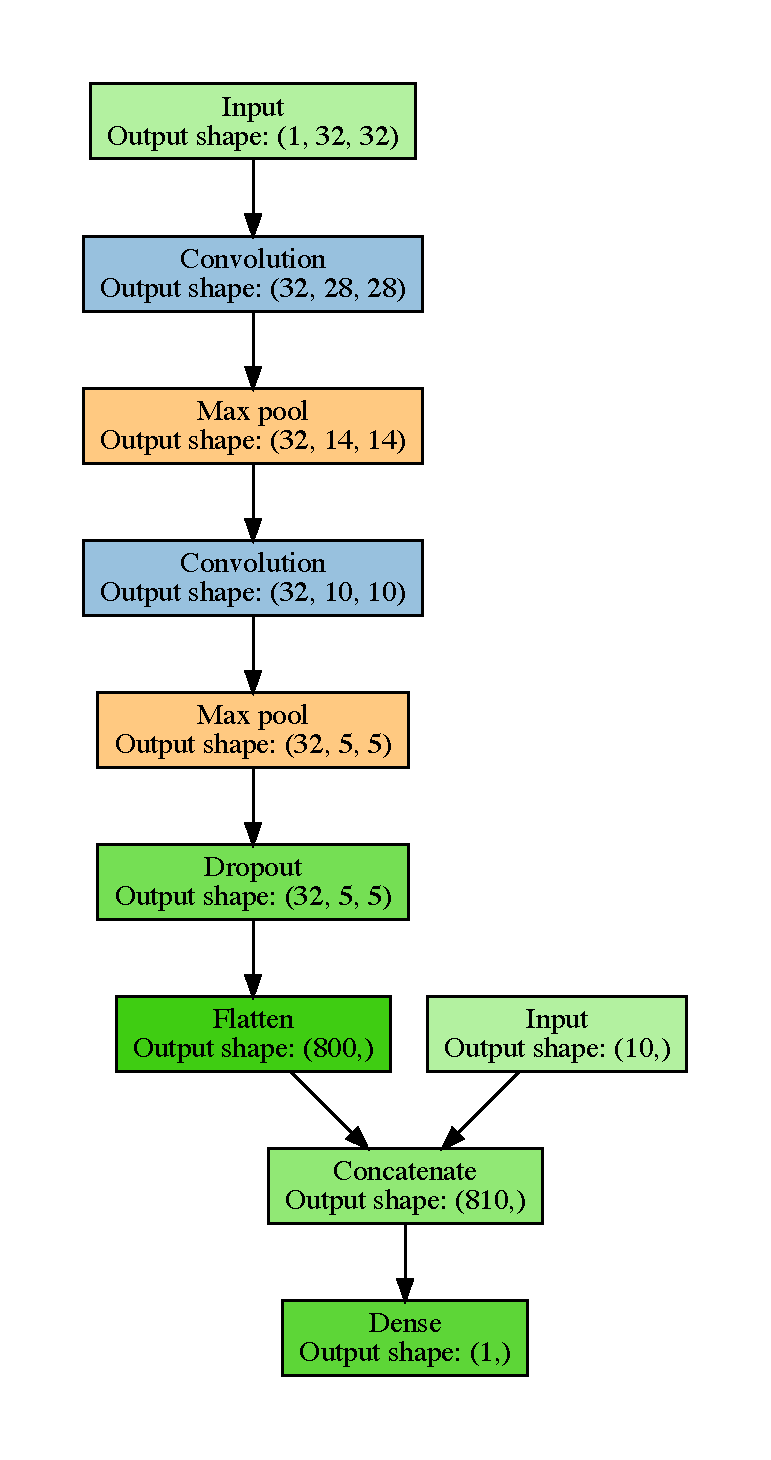
\includegraphics[height=0.9\textheight]{atlas-images/cnn_model_graph}
      \caption[Architecture of our CNN.]{Architecture of our CNN. {Parenthesised numbers indicate
      the size of output layers as a tuple (width, height, depth).} The
      concatenate layer flattens the output of the previous layer and adds the
      10 features derived from the candidate host in SWIRE, i.e. the flux
      ratios, stellarity indices, and distances. The dropout layer randomly
      sets $25$ per cent of its inputs to zero during training to prevent
      overfitting. Diagram based on \url{ https://github.com/dnouri/nolearn}.}
      \label{fig:cnn}
    \end{figure}

    CNNs have recently produced good results on large image-based datasets in
    astronomy \citep[e.g.]{lukic18compact, dieleman15cnn}. We employed
    only a simple CNN model in \autoref{cha:cross-id} as a proof of concept that CNNs may
    be used for class probability prediction on radio images. The model
    architecture we used is shown in \autoref{fig:cnn}.

  \subsection{Random forests}
  \label{sec:atlas-random-forests}

    Random forests are an ensemble of decision
    trees~\citep{breiman01random-forest}. They consider multiple subsamples of
    the training set, where each subsample is sampled with replacement from
    the training set. For each subsample a decision tree classifier is
    constructed by repeatedly making axis-parallel splits based on individual
    features. In a random forest the split decision is taken based on a random
    subset of features. To classify a new data point, the random forest takes
    the weighted average of all classifications produced by each decision
    tree. {In \autoref{cha:cross-id} we used the \texttt{scikit-learn} \citep{pedregosa11sklearn}
    implementation of random forests with 10 trees, the information entropy
    split criterion, a minimum leaf size of 45, and balanced classes}.

\section{Accuracy tables}\label{sec:atlas-xid-accuracies}
  
  This section contains tables of accuracy for our cross-identification method applied to CDFS and
  ELAIS-S1. In \autoref{tab:cdfs-ba} and \autoref{tab:elais-ba} we list the
  balanced accuracies of our \autoref{cha:cross-id} classifiers on the cross-identification task for CDFS
  and ELAIS-S1 respectively, averaged over each set of training quadrants. In
  \autoref{tab:cdfs-acc} and \autoref{tab:elais-acc} we list the balanced
  accuracies of classifiers on the cross-identification task for CDFS and
  ELAIS-S1 respectively, averaged over each set of training quadrants.

  \begin{table*}
    \caption[Balanced accuracies for different binary classification models on CDFS.]{Balanced accuracies for different binary classification models trained and tested on SWIRE objects in CDFS.
    The `Labeller' column states which set of training labels
    were used to train the classifier, and the `Classifier' column states which
    classification model was used. `CNN' is a convolutional neural network,
    `LR' is logistic regression, and `RF' is random forests. Accuracies are evaluated against the expert
    label set derived from \citet{norris06}. The standard deviation of balanced accuracies evaluated across the four quadrants of
    CDFS (\autoref{fig:quadrants}) is also shown. The `compact' set refers to SWIRE
    objects within $1'$ of a compact radio component, the `resolved' set refers to
    SWIRE objects within $1'$ of a resolved radio component, and `all' is the union of these sets.}
    \label{tab:cdfs-ba}
    \small\centering
    \begingroup
    \setlength{\tabcolsep}{8pt} % Default value: 6pt
    \begin{tabular}{ccccc}
    \hline\hline
    Labeller & Classifier & Mean `Compact' & Mean `Resolved' & Mean `All'\\
     &  & accuracy & accuracy & accuracy\\
     &  & (per cent) & (per cent) & (per cent)\\
    \hline
    Norris & LR & $91.5 \pm 1.0$ & $93.2 \pm 1.0$ & $93.0 \pm 1.2$\\
     & CNN & $92.6 \pm 0.7$ & $91.2 \pm 0.5$ & $92.0 \pm 0.6$\\
     & RF & $96.7 \pm 1.5$ & $91.0 \pm 4.5$ & $96.0 \pm 2.5$\\
    RGZ & LR & $89.5 \pm 0.8$ & $90.5 \pm 1.7$ & $90.2 \pm 0.8$\\
     & CNN & $89.4 \pm 0.6$ & $89.6 \pm 1.3$ & $89.4 \pm 0.5$\\
     & RF & $94.5 \pm 0.2$ & $95.8 \pm 0.4$ & $94.7 \pm 0.3$\\
    \hline\hline
    \end{tabular}
    \endgroup
  \end{table*}

  \begin{table*}
    \caption[Balanced accuracies for different binary classification models on ELAIS-S1.]{Balanced accuracies for different binary classification models trained on SWIRE objects
    in CDFS and tested on SWIRE objects in ELAIS-S1. Columns and abbreviations are as in \autoref{tab:cdfs-ba}. Accuracies are evaluated against the expert
    label set derived from \citet{middelberg08}. The standard deviations of balanced accuracies of models trained on the four subsets of
    CDFS (\autoref{fig:quadrants}) are also shown.}
    \label{tab:elais-ba}
    \small\centering
    \begingroup
    \setlength{\tabcolsep}{8pt} % Default value: 6pt
    \begin{tabular}{ccccc}
      \hline\hline
      Labeller & Classifier & Mean `Compact' & Mean `Resolved' & Mean `All'\\
        &  & accuracy & accuracy & accuracy\\
        &  & (per cent) & (per cent) & (per cent)\\
      \hline
      Norris & LR & $94.6 \pm 0.4$ & $93.3 \pm 2.0$ & $95.3 \pm 0.1$\\
       & CNN & $94.8 \pm 0.2$ & $92.8 \pm 0.5$ & $94.4 \pm 0.2$\\
       & RF & $85.9 \pm 3.8$ & $70.0 \pm 2.8$ & $86.6 \pm 3.2$\\
      RGZ & LR & $91.8 \pm 0.3$ & $91.9 \pm 0.5$ & $92.0 \pm 0.2$\\
       & CNN & $90.1 \pm 0.3$ & $91.1 \pm 0.9$ & $90.2 \pm 0.3$\\
       & RF & $95.1 \pm 0.1$ & $95.2 \pm 0.0$ & $95.2 \pm 0.3$\\
      \hline\hline
    \end{tabular}
    \endgroup
  \end{table*}

  \begin{table*}
    \caption[Cross-identification accuracies for different classification
    models on CDFS.]{Cross-identification accuracies for different classification
    models on CDFS. The `Labeller' column states which set of training labels
    were used to train the method, and the `Classifier' column states which
    classification model was used. `CNN' is a convolutional neural network,
    `LR' is logistic regression, `RF' is random forests, and `Labels' is the
    accuracy of the label set itself. `Perfect' indicates that the true labels
    of the test set were used and hence represents an upper bound on
    cross-identification accuracy with our method. `NN' is a
    nearest neighbours approach. Accuracies are evaluated against the expert
    label set, so `Norris' labels are 100 per cent accurate by definition. The
    standard deviation of accuracies evaluated across the four quadrants of
    CDFS (\autoref{fig:quadrants}) is also shown.}
    \label{tab:cdfs-acc}
    \small\centering
    \begingroup
    \setlength{\tabcolsep}{8pt} % Default value: 6pt
    \begin{tabular}{ccccc}
      \hline\hline
      Labeller & Classifier & Mean `Compact' & Mean `Resolved' & Mean `All'\\
       &  & accuracy & accuracy & accuracy\\
       &  & (per cent) & (per cent) & (per cent)\\
      \hline
     ---& NN & $97.2 \pm 1.7$ & $75.7 \pm 7.9$ & $93.4 \pm 0.8$\\
     ---& Random & $97.9 \pm 2.2$ & $22.3 \pm 9.2$ & $83.2 \pm 4.7$\\
      Norris & Labels & $100.0 \pm 0.0$ & $100.0 \pm 0.0$ & $100.0 \pm 0.0$\\
             & Perfect & $97.9 \pm 2.2$ & $99.0 \pm 1.8$ & $98.1 \pm 1.7$\\
             & LR & $97.3 \pm 0.5$ & $76.0 \pm 3.2$ & $93.7 \pm 1.8$\\
             & CNN & $96.6 \pm 0.9$ & $74.3 \pm 12.3$ & $93.5 \pm 0.5$\\
             & RF & $96.1 \pm 1.4$ & $75.8 \pm 6.7$ & $93.8 \pm 2.0$\\
      RGZ & Labels & $53.1 \pm 8.5$ & $56.7 \pm 5.9$ & $54.4 \pm 5.9$\\
          & LR & $97.3 \pm 1.9$ & $74.5 \pm 5.1$ & $93.6 \pm 1.7$\\
          & CNN & $85.4 \pm 2.6$ & $68.1 \pm 9.2$ & $92.4 \pm 1.1$\\
          & RF & $97.5 \pm 0.9$ & $74.3 \pm 7.9$ & $93.7 \pm 1.5$\\
      \hline\hline
    \end{tabular}
    \endgroup
  \end{table*}

  \begin{table*}
    \caption[Cross-identification accuracies for different classification
    models on ELAIS-S1.]{Cross-identification accuracies for different classification
    models on ELAIS-S1. Columns and abbreviations are as in
    \autoref{tab:cdfs-acc}. Accuracies are evaluated against the expert label
    set derived from \citet{middelberg08} cross-identifications. The standard
    deviation of accuracies evaluated across models trained on the four
    quadrants of CDFS (\autoref{fig:quadrants}) is also shown.}
    \label{tab:elais-acc}
    \small\centering
    \begingroup
    \setlength{\tabcolsep}{8pt} % Default value: 6pt
    \begin{tabular}{ccccc}
      \hline\hline
      Labeller & Classifier & Mean `Compact' & Mean `Resolved' & Mean `All'\\
       &  & accuracy & accuracy & accuracy\\
       &  & (per cent) & (per cent) & (per cent)\\
      \hline
     ---& NN & $95.5 \pm 0.0$ & $92.8 \pm 0.0$ & $95.5 \pm 0.0$\\
     ---& Random & $61.9 \pm 1.1$ & $26.6 \pm 2.1$ & $61.9 \pm 1.1$\\
      Middelberg & Perfect & $99.6 \pm 0.0$ & $99.8 \pm 0.0$ & $99.6 \pm 0.0$\\
      Norris & LR & $89.0 \pm 1.1$ & $89.7 \pm 1.8$ & $94.4 \pm 0.9$\\
             & CNN & $89.7 \pm 0.3$ & $89.4 \pm 1.4$ & $94.3 \pm 0.7$\\
             & RF & $83.8 \pm 5.6$ & $82.3 \pm 4.1$ & $90.6 \pm 2.1$\\
      RGZ & LR & $90.5 \pm 1.0$ & $92.7 \pm 0.2$ & $95.9 \pm 0.1$\\
          & CNN & $84.6 \pm 0.6$ & $84.6 \pm 0.6$ & $91.8 \pm 0.3$\\
          & RF & $91.3 \pm 1.0$ & $90.3 \pm 2.4$ & $94.7 \pm 1.2$\\
      \hline\hline
    \end{tabular}
    \endgroup
  \end{table*}

\section{SWIRE object scores}\label{sec:atlas-xid-scores}
  
  This appendix contains scores predicted by our \autoref{cha:cross-id} binary classifiers for each
  SWIRE object within $1'$ of a radio component in CDFS and ELAIS-S1. Scores
  for SWIRE~CDFS objects are shown in \autoref{tab:cdfs-scores} and scores for
  SWIRE~ELAIS-S1 are shown in \autoref{tab:elais-scores}. For CDFS, the score
  for an object in a quadrant is predicted by binary classifiers trained on
  all other quadrants. For ELAIS-S1, we show the scores predicted by binary
  classifiers trained on each CDFS quadrant. Note that these scores have
  \emph{not} been weighted by Gaussians. These are partial tables, and the full tables are available online at the \emph{Monthly Notices of the Royal Astronomical Society} website\footnote{\url{https://doi.org/10.1093/mnras/sty1308}}.

  The columns of the score tables are defined as follows:
  \begin{itemize}
    \item \emph{SWIRE}: SWIRE designation for candidate host galaxy.
    \item \emph{RA}: Right ascension (J2000).
    \item \emph{Dec}: Declination (J2000).
    \item \emph{Expert host}: Whether the candidate host galaxy is a host galaxy according to \citet{norris06} or \citet{middelberg08} cross-identifications of CDFS and ELAIS-S1 respectively.
    \item \emph{RGZ host}: Whether the candidate host galaxy is a host galaxy according to Radio Galaxy Zoo cross-identifications \citep{wong21rgz}. This is always `no' for ELAIS-S1 objects.
    \item \emph{$C$/$L$/$D$}: Score assigned by binary classifier $C$ trained on label set $L$ of $D$ candidate host galaxies. $C$ may be `CNN', `LR', or `RF' for CNN, logistic regression, or random forests respectively. $L$ may be `Norris' or `RGZ' for expert and Radio Galaxy Zoo labels respectively. $D$ may be `All', `Compact', or `Resolved' for each respective subset defined in \autoref{sec:atlas-xid-experimental-setup}.
  \end{itemize}

  \begin{sidewaystable}
    \caption[Scores output by our trained classifiers for SWIRE~CDFS candidate host galaxies.]{Scores output by our trained classifiers for SWIRE~CDFS candidate host galaxies. Columns are defined in \aref{sec:atlas-xid-scores}. Full table electronic.}
    \label{tab:cdfs-scores}
    \small\centering
    \begin{tabular}{ccccccccccc}
      \hline\hline
SWIRE & RA & Dec & Expert & RGZ & \multicolumn{6}{c}{CNN}\\
& & & host & host & \multicolumn{3}{c}{Norris} & \multicolumn{3}{c}{RGZ}\\
& & & & & All & Compact & Resolved & All & Compact & Resolved\\
      \hline
J032603.15-284708.5 & 51.5132 & -28.7857 & yes & no & 0.5838 & 0.4697 & 0.4848 & 0.3754 & 0.3881 & 0.3404 \\
J032603.39-284010.1 & 51.5142 & -28.6695 & no & no & 0.0373 & 0.5814 & 0.4878 & 0.7896 & 0.7616 & 0.4668 \\
J032603.44-284210.1 & 51.5144 & -28.7028 & no & no & 0.0232 & 0.4891 & 0.5101 & 0.4319 & 0.4298 & 0.3474 \\
J032603.44-284222.2 & 51.5143 & -28.7062 & no & no & 0.0006 & 0.4164 & 0.5216 & 0.0400 & 0.0444 & 0.0276 \\
J032603.45-284748.4 & 51.5144 & -28.7968 & no & no & 0.0014 & 0.4914 & 0.4865 & 0.1904 & 0.1895 & 0.1467 \\
J032603.50-284637.0 & 51.5146 & -28.7770 & no & no & 0.0074 & 0.4144 & 0.5382 & 0.1418 & 0.1515 & 0.1166 \\
J032603.60-284627.4 & 51.5150 & -28.7743 & no & no & 0.0012 & 0.4578 & 0.5165 & 0.0850 & 0.0904 & 0.0484 \\
J032603.63-283840.5 & 51.5151 & -28.6446 & no & no & 0.0021 & 0.4153 & 0.5577 & 0.1678 & 0.1746 & 0.1323 \\
J032603.66-283822.8 & 51.5153 & -28.6397 & no & no & 0.0001 & 0.4752 & 0.5009 & 0.0864 & 0.0861 & 0.0613 \\
J032603.75-284014.1 & 51.5156 & -28.6706 & no & no & 0.0547 & 0.3408 & 0.5388 & 0.4889 & 0.5242 & 0.7301 \\
      \hline\hline
    \end{tabular}\\
    \begin{tabular}{cccccccccccc}
      \hline\hline
\multicolumn{6}{c}{LR} & \multicolumn{6}{c}{RF} \\
\multicolumn{3}{c}{Norris} & \multicolumn{3}{c}{RGZ} & \multicolumn{3}{c}{Norris} & \multicolumn{3}{c}{RGZ} \\
All & Compact & Resolved & All & Compact & Resolved & All & Compact & Resolved & All & Compact & Resolved \\
      \hline
0.2489 & 0.0009 & 0.1557 & 0.2939 & 0.0007 & 0.1174 & 0.8922 & 0.8018 & 0.8732 & 0.7167 & 0.6599 & 0.7801 \\
0.0183 & 0.1646 & 0.1480 & 0.7637 & 0.7065 & 0.6070 & 0.0000 & 0.0000 & 0.0000 & 0.1629 & 0.0519 & 0.1275 \\
0.0155 & 0.0164 & 0.0815 & 0.3714 & 0.5626 & 0.2488 & 0.0000 & 0.0734 & 0.0000 & 0.1315 & 0.2116 & 0.4150 \\
0.0005 & 0.0006 & 0.0175 & 0.0460 & 0.0810 & 0.0299 & 0.2656 & 0.1418 & 0.0000 & 0.7631 & 0.8166 & 0.5378 \\
0.0013 & 0.0037 & 0.0160 & 0.1792 & 0.0663 & 0.1821 & 0.0000 & 0.0000 & 0.0000 & 0.0255 & 0.0000 & 0.0000 \\
0.0047 & 0.0010 & 0.0337 & 0.1284 & 0.2198 & 0.0694 & 0.0720 & 0.0000 & 0.0000 & 0.6240 & 0.6681 & 0.6704 \\
0.0008 & 0.0006 & 0.0374 & 0.1053 & 0.1424 & 0.0807 & 0.1231 & 0.0876 & 0.0000 & 0.8517 & 0.7532 & 0.7019 \\
0.0021 & 0.0073 & 0.0386 & 0.1482 & 0.0403 & 0.1210 & 0.0000 & 0.0532 & 0.0000 & 0.0000 & 0.0302 & 0.0000 \\
0.0001 & 0.0004 & 0.0038 & 0.0854 & 0.0447 & 0.0514 & 0.0000 & 0.0000 & 0.0000 & 0.0000 & 0.0000 & 0.0000 \\
0.0542 & 0.2712 & 0.2318 & 0.5026 & 0.5631 & 0.5032 & 0.0595 & 0.0545 & 0.0000 & 0.4289 & 0.0789 & 0.1420 \\
      \hline\hline
    \end{tabular}
  \end{sidewaystable}

  \begin{sidewaystable}
    \caption[Scores output by our trained classifiers for SWIRE~ELAIS-S1 candidate host galaxies.]{Scores output by our trained classifiers for SWIRE~ELAIS-S1 candidate host galaxies. Columns are defined in \aref{sec:atlas-xid-scores}. Full table electronic.}
    \label{tab:elais-scores}
    \small\centering
    \begin{tabular}{ccccccccccc}
      \hline\hline
SWIRE & RA & Dec & Expert & RGZ & \multicolumn{6}{c}{CNN} \\
 & & & host & host & \multicolumn{3}{c}{Norris} & \multicolumn{3}{c}{RGZ} \\
 & & & & & All & Compact & Resolved & All & Compact & Resolved \\
      \hline
J002925.73-440256.2 & 7.3572 & -44.0490 & yes & no & 0.9537 & 0.8638 & 0.5552 & 0.9195 & 0.9037 & 0.9371\\
J002926.14-440249.0 & 7.3590 & -44.0470 & no & no & 0.7361 & 0.8752 & 0.5640 & 0.7740 & 0.7474 & 0.7952\\
J002926.52-440247.0 & 7.3605 & -44.0464 & no & no & 0.3390 & 0.8338 & 0.5556 & 0.7275 & 0.6894 & 0.7197\\
J002926.63-440301.1 & 7.3610 & -44.0503 & no & no & 0.2108 & 0.8251 & 0.5623 & 0.3434 & 0.3306 & 0.3292\\
J002927.13-440232.6 & 7.3631 & -44.0424 & no & no & 0.0339 & 0.8479 & 0.5669 & 0.5853 & 0.5148 & 0.5159\\
J002927.28-440245.3 & 7.3637 & -44.0459 & no & no & 0.0406 & 0.8345 & 0.5540 & 0.2702 & 0.2340 & 0.2133\\
J002927.44-440238.5 & 7.3644 & -44.0440 & no & no & 0.0116 & 0.8267 & 0.5746 & 0.2228 & 0.2182 & 0.2028\\
J002928.08-440230.3 & 7.3670 & -44.0418 & no & no & 0.0024 & 0.8626 & 0.5791 & 0.2297 & 0.1963 & 0.1549\\
J002928.11-440312.7 & 7.3671 & -44.0535 & no & no & 0.0011 & 0.8159 & 0.5514 & 0.0377 & 0.0384 & 0.0271\\
J002928.80-440306.8 & 7.3700 & -44.0519 & no & no & 0.0003 & 0.8405 & 0.5668 & 0.0236 & 0.0226 & 0.0136\\
      \hline\hline
    \end{tabular}\\
    \begin{tabular}{cccccccccccc}
      \hline\hline
\multicolumn{6}{c}{LR} & \multicolumn{6}{c}{RF} \\
\multicolumn{3}{c}{LR} & \multicolumn{3}{c}{LR} & \multicolumn{3}{c}{RF} & \multicolumn{3}{c}{RF} \\
All & Compact & Resolved & All & Compact & Resolved & All & Compact & Resolved & All & Compact & Resolved \\
      \hline
0.9722 & 0.9955 & 0.8769 & 0.9933 & 0.9934 & 0.9658 & 0.8824 & 0.9664 & 0.7950 & 0.8078 & 0.9227 & 0.7677 \\
0.4669 & 0.0111 & 0.4249 & 0.3926 & 0.2220 & 0.5947 & 0.2077 & 0.0000 & 0.1613 & 0.1876 & 0.0852 & 0.4546 \\
0.2264 & 0.0254 & 0.2389 & 0.6275 & 0.3033 & 0.6812 & 0.1347 & 0.0857 & 0.0399 & 0.3582 & 0.4854 & 0.5347 \\
0.0603 & 0.0007 & 0.0734 & 0.0688 & 0.0141 & 0.1581 & 0.0917 & 0.0000 & 0.0399 & 0.2846 & 0.1245 & 0.2833 \\
0.0248 & 0.0334 & 0.0301 & 0.5735 & 0.5065 & 0.5265 & 0.1977 & 0.1507 & 0.0000 & 0.3334 & 0.6593 & 0.3995 \\
0.0173 & 0.0016 & 0.0359 & 0.1056 & 0.0492 & 0.1456 & 0.0000 & 0.0000 & 0.0000 & 0.0000 & 0.0000 & 0.0287 \\
0.0064 & 0.0049 & 0.0187 & 0.1981 & 0.1534 & 0.1493 & 0.0000 & 0.0000 & 0.0000 & 0.1565 & 0.1634 & 0.1284 \\
0.0020 & 0.0005 & 0.0239 & 0.1337 & 0.1001 & 0.1310 & 0.0000 & 0.0000 & 0.0358 & 0.0000 & 0.0000 & 0.0190 \\
0.0008 & 0.0013 & 0.0119 & 0.0280 & 0.0361 & 0.0205 & 0.1171 & 0.0000 & 0.0000 & 0.0873 & 0.0383 & 0.0000 \\
0.0004 & 0.0014 & 0.0095 & 0.0339 & 0.0408 & 0.0136 & 0.0000 & 0.0000 & 0.0000 & 0.1114 & 0.1480 & 0.1584 \\
      \hline\hline
    \end{tabular}
  \end{sidewaystable}

\section{ATLAS component cross-identifications}\label{sec:atlas-xid-xids}
  
  This section contains cross-identifications predicted by our cross-identification method for each
  ATLAS radio component in CDFS and ELAIS-S1. Cross-identifications for
  ATLAS~CDFS components are shown in \autoref{tab:cdfs-xids} and
  cross-identifications for ATLAS~ELAIS-S1 are shown in
  \autoref{tab:elais-xids}. For CDFS, the cross-identification for a component
  in a quadrant is predicted using our method with binary classifiers trained
  on all other quadrants. For ELAIS-S1, we show the cross-identifications
  predicted by our method using binary classifiers trained on each CDFS
  quadrant. For CDFS, we also show the Radio Galaxy Zoo consensus, which is a
  proxy for the difficulty of cross-identifying a component \citep{wong21rgz}. These are partial tables, and the full tables are available online at the \emph{Monthly Notices of the Royal Astronomical Society} website\footnote{\url{https://doi.org/10.1093/mnras/sty1308}}.

  The columns of the cross-identification tables are defined as follows:
  \begin{itemize}
    \item \emph{ATLAS}: ATLAS designation for radio component.
    \item \emph{RA}: Right ascension of radio component (J2000).
    \item \emph{Dec}: Declination of radio component (J2000).
    \item \emph{CID}: Radio Galaxy Zoo component ID.
    \item \emph{Zooniverse ID}: Radio Galaxy Zoo Zooniverse ID.
    \item \emph{Norris/Middelberg}: Designation of SWIRE cross-identification from \citet{norris06} or \citet{middelberg08} for CDFS and ELAIS-S1 respectively.
    \item \emph{Norris/Middelberg RA}: Right ascension of SWIRE cross-identification from \citet{norris06} or \citet{middelberg08} for CDFS and ELAIS-S1 respectively.
    \item \emph{Norris/Middelberg Dec}: Right ascension of SWIRE cross-identification from \citet{norris06} or \citet{middelberg08} for CDFS and ELAIS-S1 respectively.
    \item \emph{RGZ}: Designation of SWIRE cross-identification from Radio Galaxy Zoo \citep{wong21rgz}.
    \item \emph{RGZ RA}: Right ascension of SWIRE cross-identification from Radio Galaxy Zoo \citep{wong21rgz}.
    \item \emph{RGZ Dec}: Right ascension of SWIRE cross-identification from Radio Galaxy Zoo \citep{wong21rgz}.
    \item \emph{RGZ radio consensus}: Percentage agreement of Radio Galaxy Zoo volunteers on the radio component configuration.
    \item \emph{RGZ IR consensus}: Percentage agreement of Radio Galaxy Zoo volunteers on the host galaxy of this radio component.
    \item \emph{$C$ / $L$ / $D$}: Designation of SWIRE cross-identification made by our method using classification model $C$ trained on label set $L$ of $D$ candidate host galaxies. $C$ may be `CNN', `LR', or `RF' for CNN, logistic regression or random forests respectively. $L$ may be `Norris' or `RGZ' for expert and Radio Galaxy Zoo labels respectively. $D$ may be `All', `Compact', or `Resolved' for each respective subset defined in \autoref{sec:atlas-xid-experimental-setup}.
    \item \emph{$C$/ $L$ / $D$ RA}: Right ascension (J2000) of SWIRE cross-identification made by our method using classification model $C$ trained on label set $L$ of $D$ candidate host galaxies. $C$, $L$, and $D$ are defined as for designation.
    \item \emph{$C$/ $L$ / $D$ Dec}: Declination (J2000) of SWIRE cross-identification made by our method using classification model $C$ trained on label set $L$ of $D$ candidate host galaxies. $C$, $L$, and $D$ are defined as for designation.
  \end{itemize}

  \begin{sidewaystable}
    \caption[Cross-identifications for ATLAS~CDFS components.]{Cross-identifications for ATLAS~CDFS components. Columns are defined in \aref{sec:atlas-xid-xids}. Full table electronic.}
    \label{tab:cdfs-xids}
    \tiny\centering
    \begin{tabular}{ccccccccccccc}
      \hline\hline
ATLAS & RA & Dec & CID & Zooniverse & \multicolumn{3}{c}{Norris} & \multicolumn{3}{c}{RGZ} & \multicolumn{2}{c}{RGZ}\\
 & & & & ID & & RA & Dec & & RA & Dec & radio & IR \\
 & & & & & & RA & Dec & & RA & Dec & consensus & consensus\\
      \hline
J032602.82-284708.1C & 51.5117 & -28.7856 & CI0412 & ARG0003rb2 & J032603.15-284708.5 & 51.5132 & -28.7857 &  &  &  & 0.4516 & 0.3214 \\
J032615.49-284629.4C & 51.5646 & -28.7749 & CI0614 & ARG0003rfr & J032615.41-284630.7 & 51.5642 & -28.7752 & J032615.41-284630.7 & 51.5642 & -28.7752 & 0.2941 & 0.8000 \\
J032615.55-280559.8C & 51.5648 & -28.1000 & CI0320 & ARG0003r8s & J032615.52-280559.8 & 51.5647 & -28.1000 & J032615.52-280559.8 & 51.5647 & -28.1000 & 0.5625 & 0.8333 \\
J032617.35-280710.2C & 51.5723 & -28.1195 & CI0059C1 & ARG0003r2j & J032617.89-280707.2 & 51.5746 & -28.1187 & J032617.89-280707.2 & 51.5746 & -28.1187 & 0.4146 & 1.0000 \\
J032625.13-280909.8C & 51.6047 & -28.1527 & CI0409 & ARG0003raz & J032625.19-280910.1 & 51.6050 & -28.1528 & J032625.19-280910.1 & 51.6050 & -28.1528 & 0.3158 & 0.6667 \\
J032629.10-280650.1C & 51.6213 & -28.1139 & CI0963 & ARG0003ro4 & J032629.13-280650.7 & 51.6214 & -28.1141 & J032626.74-280636.7 & 51.6114 & -28.1102 & 0.3333 & 1.0000 \\
J032629.61-284052.7C & 51.6234 & -28.6813 & CI0304 & ARG0003r8e & J032629.54-284055.8 & 51.6231 & -28.6822 & J032629.54-284055.8 & 51.6231 & -28.6822 & 0.2676 & 1.0000 \\
J032629.92-284753.5C & 51.6247 & -28.7982 & CI0120 & ARG0003r3w & J032629.81-284754.4 & 51.6242 & -28.7985 & J032629.81-284754.4 & 51.6242 & -28.7985 & 1.0000 & 0.8571 \\
J032630.66-283657.3C & 51.6278 & -28.6159 & CI0172C1 & ARG0003r55 & J032630.64-283658.0 & 51.6277 & -28.6161 & J032628.56-283744.8 & 51.619 & -28.6291 & 0.3611 & 0.7308 \\
J032634.59-282022.8C & 51.6441 & -28.3397 & CI0757 & ARG0003rj2 & J032634.58-282022.8 & 51.6441 & -28.3397 & J032631.96-281941.0 & 51.6332 & -28.3281 & 0.5781 & 0.5405 \\
      \hline\hline
    \end{tabular}
    \begin{tabular}{cccccccccccc}
      \hline\hline
\multicolumn{12}{c}{CNN}\\
 \multicolumn{3}{c}{Compact} & \multicolumn{3}{c}{Resolved} & \multicolumn{3}{c}{Compact} & \multicolumn{3}{c}{Resolved}\\
 & RA & Dec & & RA & Dec & & RA & Dec & & RA & Dec\\
      \hline
J032602.36-284711.5 & 51.5098 & -28.7865 & J032602.36-284711.5 & 51.5098 & -28.7865 & J032602.36-284711.5 & 51.5098 & -28.7865 & J032602.36-284711.5 & 51.5098 & -28.7865\\
J032615.41-284630.7 & 51.5642 & -28.7752 & J032615.41-284630.7 & 51.5642 & -28.7752 & J032615.41-284630.7 & 51.5642 & -28.7752 & J032615.41-284630.7 & 51.5642 & -28.7752\\
J032615.52-280559.8 & 51.5647 & -28.1000 & J032615.52-280559.8 & 51.5647 & -28.1000 & J032615.52-280559.8 & 51.5647 & -28.1000 & J032615.52-280559.8 & 51.5647 & -28.1000\\
J032617.89-280707.2 & 51.5746 & -28.1187 & J032617.89-280707.2 & 51.5746 & -28.1187 & J032617.89-280707.2 & 51.5746 & -28.1187 & J032617.89-280707.2 & 51.5746 & -28.1187\\
J032625.19-280910.1 & 51.6050 & -28.1528 & J032625.19-280910.1 & 51.6050 & -28.1528 & J032624.50-280905.9 & 51.6021 & -28.1517 & J032625.19-280910.1 & 51.6050 & -28.1528\\
J032629.13-280650.7 & 51.6214 & -28.1141 & J032629.13-280650.7 & 51.6214 & -28.1141 & J032629.13-280650.7 & 51.6214 & -28.1141 & J032629.13-280650.7 & 51.6214 & -28.1141\\
J032629.54-284051.9 & 51.6231 & -28.6811 & J032629.54-284051.9 & 51.6231 & -28.6811 & J032629.54-284051.9 & 51.6231 & -28.6811 & J032629.54-284051.9 & 51.6231 & -28.6811\\
J032629.81-284754.4 & 51.6242 & -28.7985 & J032629.81-284754.4 & 51.6242 & -28.7985 & J032629.81-284754.4 & 51.6242 & -28.7985 & J032629.81-284754.4 & 51.6242 & -28.7985\\
J032630.64-283658.0 & 51.6277 & -28.6161 & J032630.64-283658.0 & 51.6277 & -28.6161 & J032630.64-283658.0 & 51.6277 & -28.6161 & J032630.64-283658.0 & 51.6277 & -28.6161\\
J032634.58-282022.8 & 51.6441 & -28.3397 & J032634.58-282022.8 & 51.6441 & -28.3397 & J032634.58-282022.8 & 51.6441 & -28.3397 & J032634.58-282022.8 & 51.6441 & -28.3397\\
      \hline\hline
    \end{tabular}\\
    \begin{tabular}{cccccccccccc}
      \hline\hline
\multicolumn{12}{c}{LR}\\
 \multicolumn{6}{c}{Norris} & \multicolumn{6}{c}{RGZ}\\
 \multicolumn{3}{c}{Compact} & \multicolumn{3}{c}{Resolved} & \multicolumn{3}{c}{Compact} & \multicolumn{3}{c}{Resolved} \\
  & RA & Dec & & RA & Dec & & RA & Dec & & RA & Dec \\
      \hline
J032604.58-284650.9 & 51.5191 & -28.7808 & J032602.08-284713.1 & 51.5087 & -28.787 & J032602.36-284711.5 & 51.5098 & -28.7865 & J032602.36-284711.5 & 51.5098 & -28.7865\\
J032615.41-284630.7 & 51.5642 & -28.7752 & J032615.41-284630.7 & 51.5642 & -28.7752 & J032615.41-284630.7 & 51.5642 & -28.7752 & J032615.41-284630.7 & 51.5642 & -28.7752\\
J032615.52-280559.8 & 51.5647 & -28.1000 & J032615.52-280559.8 & 51.5647 & -28.1000 & J032615.52-280559.8 & 51.5647 & -28.1000 & J032615.52-280559.8 & 51.5647 & -28.1000\\
J032615.86-280628.8 & 51.5661 & -28.1080 & J032615.16-280742.2 & 51.5632 & -28.1284 & J032615.86-280628.8 & 51.5661 & -28.1080 & J032618.84-280722.6 & 51.5785 & -28.1230\\
J032625.19-280910.1 & 51.6050 & -28.1528 & J032625.19-280910.1 & 51.6050 & -28.1528 & J032625.19-280910.1 & 51.6050 & -28.1528 & J032625.19-280910.1 & 51.6050 & -28.1528\\
J032629.13-280650.7 & 51.6214 & -28.1141 & J032629.13-280650.7 & 51.6214 & -28.1141 & J032629.13-280650.7 & 51.6214 & -28.1141 & J032629.13-280650.7 & 51.6214 & -28.1141\\
J032629.54-284051.9 & 51.6231 & -28.6811 & J032629.54-284051.9 & 51.6231 & -28.6811 & J032629.54-284051.9 & 51.6231 & -28.6811 & J032629.54-284051.9 & 51.6231 & -28.6811\\
J032629.81-284754.4 & 51.6242 & -28.7985 & J032629.81-284754.4 & 51.6242 & -28.7985 & J032629.81-284754.4 & 51.6242 & -28.7985 & J032629.81-284754.4 & 51.6242 & -28.7985\\
J032630.64-283658.0 & 51.6277 & -28.6161 & J032630.64-283658.0 & 51.6277 & -28.6161 & J032630.64-283658.0 & 51.6277 & -28.6161 & J032630.64-283658.0 & 51.6277 & -28.6161\\
J032634.58-282022.8 & 51.6441 & -28.3397 & J032634.58-282022.8 & 51.6441 & -28.3397 & J032634.58-282022.8 & 51.6441 & -28.3397 & J032634.58-282022.8 & 51.6441 & -28.3397\\
      \hline\hline
    \end{tabular}\\
    \begin{tabular}{cccccccccccc}
      \hline\hline
\multicolumn{12}{c}{RF} \\
 \multicolumn{6}{c}{Norris} & \multicolumn{6}{c}{RGZ} \\
 \multicolumn{3}{c}{Compact} & \multicolumn{3}{c}{Resolved} & \multicolumn{3}{c}{Compact} & \multicolumn{3}{c}{Resolved} \\
  & RA & Dec & & RA & Dec & & RA & Dec & & RA & Dec \\
      \hline
J032603.15-284708.5 & 51.5132 & -28.7857 & J032602.36-284711.5 & 51.5098 & -28.7865 & J032602.36-284711.5 & 51.5098 & -28.7865 & J032602.36-284711.5 & 51.5098 & -28.7865 \\
J032615.41-284630.7 & 51.5642 & -28.7752 & J032615.41-284630.7 & 51.5642 & -28.7752 & J032615.41-284630.7 & 51.5642 & -28.7752 & J032615.41-284630.7 & 51.5642 & -28.7752 \\
J032615.52-280559.8 & 51.5647 & -28.1000 & J032615.52-280559.8 & 51.5647 & -28.1000 & J032615.52-280559.8 & 51.5647 & -28.1000 & J032615.52-280559.8 & 51.5647 & -28.1000 \\
J032617.89-280707.2 & 51.5746 & -28.1187 & J032617.89-280707.2 & 51.5746 & -28.1187 & J032617.89-280707.2 & 51.5746 & -28.1187 & J032617.89-280707.2 & 51.5746 & -28.1187 \\
J032625.19-280910.1 & 51.6050 & -28.1528 & J032625.19-280910.1 & 51.6050 & -28.1528 & J032625.19-280910.1 & 51.6050 & -28.1528 & J032625.19-280910.1 & 51.6050 & -28.1528 \\
J032629.13-280650.7 & 51.6214 & -28.1141 & J032629.13-280650.7 & 51.6214 & -28.1141 & J032629.13-280650.7 & 51.6214 & -28.1141 & J032629.13-280650.7 & 51.6214 & -28.1141 \\
J032629.54-284051.9 & 51.6231 & -28.6811 & J032629.54-284051.9 & 51.6231 & -28.6811 & J032629.54-284051.9 & 51.6231 & -28.6811 & J032629.54-284051.9 & 51.6231 & -28.6811 \\
J032630.12-284751.2 & 51.6255 & -28.7976 & J032629.81-284754.4 & 51.6242 & -28.7985 & J032629.81-284754.4 & 51.6242 & -28.7985 & J032629.81-284754.4 & 51.6242 & -28.7985 \\
J032630.64-283658.0 & 51.6277 & -28.6161 & J032630.64-283658.0 & 51.6277 & -28.6161 & J032630.64-283658.0 & 51.6277 & -28.6161 & J032630.64-283658.0 & 51.6277 & -28.6161 \\
J032634.58-282022.8 & 51.6441 & -28.3397 & J032634.58-282022.8 & 51.6441 & -28.3397 & J032634.58-282022.8 & 51.6441 & -28.3397 & J032634.58-282022.8 & 51.6441 & -28.3397 \\
      \hline\hline
    \end{tabular}
  \end{sidewaystable}

  \begin{sidewaystable}
    \caption{Cross-identifications for ATLAS~ELAIS-S1 components. Columns are defined in \aref{sec:atlas-xid-xids}. Full table electronic.}
    \label{tab:elais-xids}
    \tiny\centering
    \begin{tabular}{ccccccccccccccccccccccccccccccccccccccccccccccccccccccccccccccccccc}
      \hline\hline
ATLAS & RA & Dec & CID & Zooniverse & \multicolumn{3}{c}{Middelberg} & \multicolumn{3}{c}{RGZ} & \multicolumn{2}{c}{RGZ}\\
 & & & & ID & & RA & Dec & & RA & Dec & radio & IR \\
 & & & & & & RA & Dec & & RA & Dec & consensus & consensus\\
      \hline
J002925.68-440256.8 & 7.3570 & -44.0491 & C0375 &  & J002925.73-440256.2 & 7.3572 & -44.0490 &  &  &  &  & \\
J002938.19-432946.7 & 7.4092 & -43.4963 & C0832 &  & J002938.07-432947.9 & 7.4087 & -43.4967 &  &  &  &  & \\
J002940.13-440309.2 & 7.4172 & -44.0526 & C0374 &  & J002940.19-440309.6 & 7.4175 & -44.0527 &  &  &  &  & \\
J002943.14-440812.3 & 7.4298 & -44.1368 & C0302 &  & J002943.15-440813.6 & 7.4298 & -44.1371 &  &  &  &  & \\
J002944.51-433627.8 & 7.4355 & -43.6077 & C0727 &  & J002944.36-433630.2 & 7.4348 & -43.6084 &  &  &  &  & \\
J002945.31-432148.5 & 7.4388 & -43.3635 & C0943.1 &  & J002945.64-432149.3 & 7.4402 & -43.3637 &  &  &  & \\
J002946.14-432149.1 & 7.4423 & -43.3637 & C0943 &  & J002945.64-432149.3 & 7.4402 & -43.3637 &  &  &  &  & \\
J002949.89-440541.4 & 7.4579 & -44.0948 & C0345 &  &  &  &  &  &  &  &  & \\
J002951.13-432354.3 & 7.4631 & -43.3984 & C0924 &  & J002951.14-432355.3 & 7.4631 & -43.3987 &  &  &  &  & \\
J002951.19-440556.6 & 7.4633 & -44.0991 & C0342 &  & J002951.26-440556.4 & 7.4636 & -44.0990 &  &  &  &  & \\
      \hline
    \end{tabular}
    \begin{tabular}{ccccccccccccccccccccccccccccccccccccccccccccccccccccccccccccccccccc}
      \hline
\multicolumn{12}{c}{CNN}\\
\multicolumn{6}{c}{Norris} & \multicolumn{6}{c}{RGZ}\\
\multicolumn{3}{c}{Compact} & \multicolumn{3}{c}{Resolved} & \multicolumn{3}{c}{Compact} & \multicolumn{3}{c}{Resolved} \\
 & RA & Dec & & RA & Dec & & RA & Dec & & RA & Dec\\
      \hline
J002925.73-440256.2 & 7.3572 & -44.0490 & J002925.73-440256.2 & 7.3572 & -44.0490 & J002925.73-440256.2 & 7.3572 & -44.0490 & J002925.73-440256.2 & 7.3572 & -44.0490\\
J002938.07-432947.9 & 7.4087 & -43.4967 & J002938.07-432947.9 & 7.4087 & -43.4967 & J002937.50-432945.4 & 7.4063 & -43.4959 & J002937.50-432945.4 & 7.4063 & -43.4959\\
J002940.19-440309.6 & 7.4175 & -44.0527 & J002940.19-440309.6 & 7.4175 & -44.0527 & J002940.19-440309.6 & 7.4175 & -44.0527 & J002940.19-440309.6 & 7.4175 & -44.0527\\
J002943.15-440813.6 & 7.4298 & -44.1371 & J002943.15-440813.6 & 7.4298 & -44.1371 & J002943.15-440813.6 & 7.4298 & -44.1371 & J002943.15-440813.6 & 7.4298 & -44.1371\\
J002944.36-433630.2 & 7.4348 & -43.6084 & J002944.36-433630.2 & 7.4348 & -43.6084 & J002944.36-433630.2 & 7.4348 & -43.6084 & J002944.36-433630.2 & 7.4348 & -43.6084\\
J002945.64-432149.3 & 7.4402 & -43.3637 & J002945.64-432149.3 & 7.4402 & -43.3637 & J002945.64-432149.3 & 7.4402 & -43.3637 & J002945.64-432149.3 & 7.4402 & -43.3637\\
J002945.64-432149.3 & 7.4402 & -43.3637 & J002945.64-432149.3 & 7.4402 & -43.3637 & J002945.64-432149.3 & 7.4402 & -43.3637 & J002945.64-432149.3 & 7.4402 & -43.3637\\
J002951.44-440546.1 & 7.4644 & -44.0962 & J002951.44-440546.1 & 7.4644 & -44.0962 & J002951.44-440546.1 & 7.4644 & -44.0962 & J002951.44-440546.1 & 7.4644 & -44.0962\\
J002951.14-432355.3 & 7.4631 & -43.3987 & J002951.14-432355.3 & 7.4631 & -43.3987 & J002951.14-432355.3 & 7.4631 & -43.3987 & J002951.14-432355.3 & 7.4631 & -43.3987\\
J002951.26-440556.4 & 7.4636 & -44.0990 & J002951.44-440546.1 & 7.4644 & -44.0962 & J002951.51-440617.1 & 7.4646 & -44.1048 & J002951.44-440546.1 & 7.4644 & -44.0962\\
      \hline
    \end{tabular}
    \begin{tabular}{ccccccccccccccccccccccccccccccccccccccccccccccccccccccccccccccccccc}
      \hline
\multicolumn{12}{c}{LR}\\
\multicolumn{6}{c}{Norris} & \multicolumn{6}{c}{RGZ}\\
\multicolumn{3}{c}{Compact} & \multicolumn{3}{c}{Resolved} & \multicolumn{3}{c}{Compact} & \multicolumn{3}{c}{Resolved}\\
 & RA & Dec & & RA & Dec & & RA & Dec & & RA & Dec\\
      \hline
J002925.73-440256.2 & 7.3572 & -44.0490 & J002925.73-440256.2 & 7.3572 & -44.0490 & J002925.73-440256.2 & 7.3572 & -44.0490 & J002925.73-440256.2 & 7.3572 & -44.0490\\
J002938.07-432947.9 & 7.4087 & -43.4967 & J002938.07-432947.9 & 7.4087 & -43.4967 & J002938.07-432947.9 & 7.4087 & -43.4967 & J002938.07-432947.9 & 7.4087 & -43.4967\\
J002940.19-440309.6 & 7.4175 & -44.0527 & J002940.19-440309.6 & 7.4175 & -44.0527 & J002940.19-440309.6 & 7.4175 & -44.0527 & J002940.19-440309.6 & 7.4175 & -44.0527\\
J002943.15-440813.6 & 7.4298 & -44.1371 & J002943.15-440813.6 & 7.4298 & -44.1371 & J002943.15-440813.6 & 7.4298 & -44.1371 & J002943.15-440813.6 & 7.4298 & -44.1371\\
J002944.36-433630.2 & 7.4348 & -43.6084 & J002944.36-433630.2 & 7.4348 & -43.6084 & J002944.36-433630.2 & 7.4348 & -43.6084 & J002944.36-433630.2 & 7.4348 & -43.6084\\
J002945.64-432149.3 & 7.4402 & -43.3637 & J002945.64-432149.3 & 7.4402 & -43.3637 & J002945.64-432149.3 & 7.4402 & -43.3637 & J002945.64-432149.3 & 7.4402 & -43.3637\\
J002945.64-432149.3 & 7.4402 & -43.3637 & J002945.64-432149.3 & 7.4402 & -43.3637 & J002945.64-432149.3 & 7.4402 & -43.3637 & J002945.64-432149.3 & 7.4402 & -43.3637\\
J002951.26-440556.4 & 7.4636 & -44.0990 & J002951.26-440556.4 & 7.4636 & -44.0990 & J002951.26-440556.4 & 7.4636 & -44.0990 & J002951.26-440556.4 & 7.4636 & -44.0990\\
J002951.14-432355.3 & 7.4631 & -43.3987 & J002951.14-432355.3 & 7.4631 & -43.3987 & J002951.14-432355.3 & 7.4631 & -43.3987 & J002951.14-432355.3 & 7.4631 & -43.3987\\
J002951.26-440556.4 & 7.4636 & -44.0990 & J002951.26-440556.4 & 7.4636 & -44.0990 & J002951.26-440556.4 & 7.4636 & -44.0990 & J002951.26-440556.4 & 7.4636 & -44.0990\\
      \hline
    \end{tabular}
    \begin{tabular}{ccccccccccccccccccccccccccccccccccccccccccccccccccccccccccccccccccc}
      \hline
\multicolumn{12}{c}{RF}\\
\multicolumn{6}{c}{Norris} & \multicolumn{6}{c}{RGZ}\\
\multicolumn{3}{c}{Compact} & \multicolumn{3}{c}{Resolved} & \multicolumn{3}{c}{Compact} & \multicolumn{3}{c}{Resolved} \\
 & RA & Dec & & RA & Dec & & RA & Dec & & RA & Dec \\
      \hline
J002925.73-440256.2 & 7.3572 & -44.0490 & J002925.73-440256.2 & 7.3572 & -44.0490 & J002925.73-440256.2 & 7.3572 & -44.0490 & J002925.73-440256.2 & 7.3572 & -44.0490 \\
J002938.07-432947.9 & 7.4087 & -43.4967 & J002938.07-432947.9 & 7.4087 & -43.4967 & J002938.07-432947.9 & 7.4087 & -43.4967 & J002938.07-432947.9 & 7.4087 & -43.4967 \\
J002940.19-440309.6 & 7.4175 & -44.0527 & J002940.19-440309.6 & 7.4175 & -44.0527 & J002940.19-440309.6 & 7.4175 & -44.0527 & J002940.19-440309.6 & 7.4175 & -44.0527 \\
J002943.15-440813.6 & 7.4298 & -44.1371 & J002943.15-440813.6 & 7.4298 & -44.1371 & J002943.15-440813.6 & 7.4298 & -44.1371 & J002943.15-440813.6 & 7.4298 & -44.1371 \\
J002944.36-433630.2 & 7.4348 & -43.6084 & J002944.36-433630.2 & 7.4348 & -43.6084 & J002944.36-433630.2 & 7.4348 & -43.6084 & J002944.36-433630.2 & 7.4348 & -43.6084 \\
J002945.64-432149.3 & 7.4402 & -43.3637 & J002945.64-432149.3 & 7.4402 & -43.3637 & J002945.64-432149.3 & 7.4402 & -43.3637 & J002945.64-432149.3 & 7.4402 & -43.3637 \\
J002945.64-432149.3 & 7.4402 & -43.3637 & J002945.64-432149.3 & 7.4402 & -43.3637 & J002945.64-432149.3 & 7.4402 & -43.3637 & J002945.64-432149.3 & 7.4402 & -43.3637 \\
J002951.26-440556.4 & 7.4636 & -44.0990 & J002951.26-440556.4 & 7.4636 & -44.0990 & J002949.13-440536.5 & 7.4547 & -44.0935 & J002949.13-440536.5 & 7.4547 & -44.0935 \\
J002951.14-432355.3 & 7.4631 & -43.3987 & J002951.14-432355.3 & 7.4631 & -43.3987 & J002951.14-432355.3 & 7.4631 & -43.3987 & J002951.14-432355.3 & 7.4631 & -43.3987 \\
J002951.26-440556.4 & 7.4636 & -44.0990 & J002951.26-440556.4 & 7.4636 & -44.0990 & J002951.26-440556.4 & 7.4636 & -44.0990 & J002951.26-440556.4 & 7.4636 & -44.0990 \\
      \hline
    \end{tabular}
  \end{sidewaystable}

\section{Cross-identification figures}\label{sec:atlas-xid-examples}

    \autoref{fig:examples} shows figures of our cross-identifications of each ATLAS radio component in CDFS and ELAIS-S1. There are just five examples shown here, but all 469 examples are available online at the \emph{Monthly Notices of the Royal Astronomical Society} website\footnote{\url{https://doi.org/10.1093/mnras/sty1308}}.


    \begin{figure}
        \centering
        \begin{subfigure}{0.45\textwidth}
            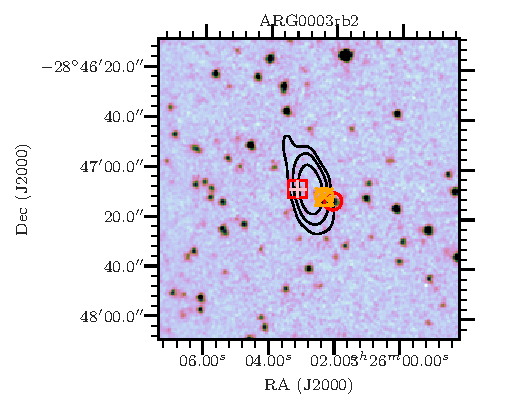
\includegraphics[width=\textwidth]{atlas-images/examples_all/example_sorted_2_0.pdf}
            \caption{One resolved component and resolved source.}
        \end{subfigure}
        \begin{subfigure}{0.45\textwidth}
            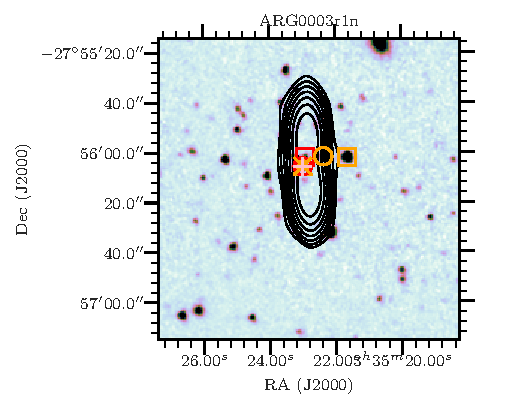
\includegraphics[width=\textwidth]{atlas-images/examples_all/example_sorted_3_454.pdf}
            \caption{Three resolved components comprising one resolved source.}
        \end{subfigure}
        \begin{subfigure}{0.45\textwidth}
            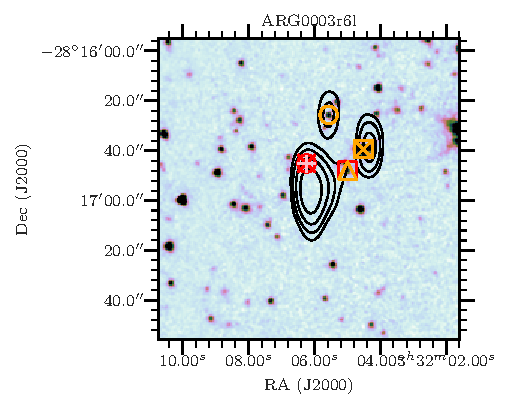
\includegraphics[width=\textwidth]{atlas-images/examples_all/example_sorted_4_264.pdf}
            \caption{Three resolved components comprising one resolved source.}
        \end{subfigure}
        \begin{subfigure}{0.45\textwidth}
            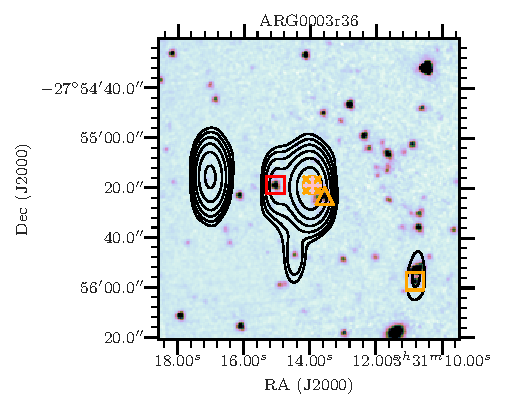
\includegraphics[width=\textwidth]{atlas-images/examples_all/example_sorted_5_207.pdf}
            \caption{Three resolved components comprising one resolved source.}
        \end{subfigure}
        \begin{subfigure}{0.9\textwidth}
            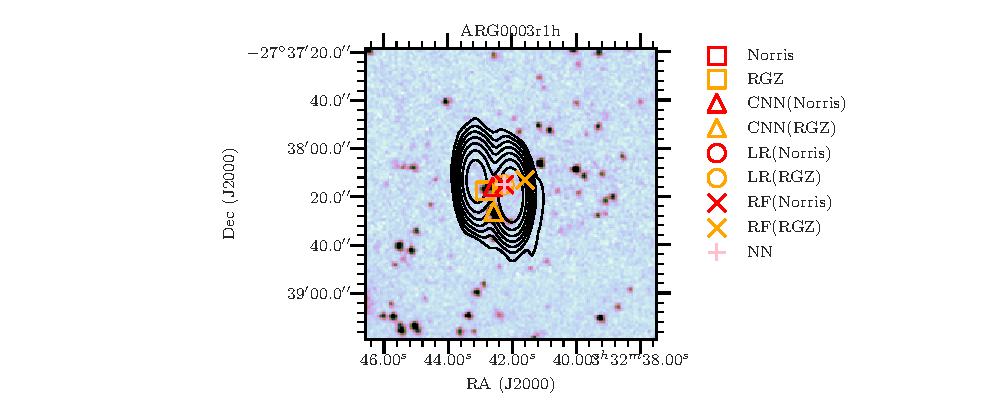
\includegraphics[width=\textwidth]{atlas-images/examples_all/example_sorted_0_306.pdf}
            \caption{Two compact components, each a compact source.}
        \end{subfigure}
        \caption[Examples of resolved sources with high disagreement between cross-identifiers.]{\label{fig:examples} Examples of resolved sources with high disagreement between cross-identifiers. The contours show ATLAS radio data and start at $4\sigma$, increasing geometrically by a factor of 2. The background image is the \unit{3.6}{\micro\meter} SWIRE image. Binary classifier model/training set combinations are denoted $C(S)$ where $C$ is the binary classifier model and $S$ is the training set. `LR' is logistic regression, `CNN' is convolutional neural networks, and `RF' is random forests. `Norris' refers to the expert labels and `RGZ' refers to the Radio Galaxy Zoo labels. The cross-identification made by nearest neighbours is shown by `NN'.}
    \end{figure}


\unappendix

%!tex root=./thesis.tex
\chapter{Radio Luminosity Functions}
\label{cha:rlfs}

\section{Radio Luminosity Functions}
\label{sec:rlfs}


\section{Making Catalogues with Binary Cross-identification}
\label{sec:revisiting-cross-id}


\section{FIRST paper...}

%!tex root=./thesis.tex
\chapter{Faraday Complexity}
\label{cha:faraday-faraday}

This chapter is based on my to-be-submitted paper \emph{Interpretable Faraday Complexity Classification}, by M. J. Alger, C. S. Ong, J. D. Livingston, J. L. Nabaglo, N. M. McClure-Griffiths, and O. I. Wong.

  Faraday complexity describes whether a spectropolarimetric observation has simple or complex magnetic structure. Quickly determining the Faraday complexity of a spectropolarimetric observation is important for processing large, polarised radio surveys. Finding simple sources lets us build rotation measure grids, and finding complex sources lets us follow these sources up with slower analysis techniques or further observations. In this chapter, we introduce five features that can be used to train simple, interpretable machine learning classifiers for estimating Faraday complexity. We train logistic regression and extreme gradient boosted tree classifiers on simulated polarised spectra using our features, analyse their behaviour, and demonstrate our features are effective for both simulated and real data. With 95 per cent accuracy on simulated ASKAP data and 90 per cent accuracy on simulated ATCA data, our method performs comparably to state-of-the-art convolutional neural networks while being simpler and easier to interpret. Logistic regression trained with our features behaves sensibly on real data and its outputs are useful for sorting polarised sources by apparent Faraday complexity.

  M.J.A. and J.D.L. were supported by the Australian Government Research Training Program. M.J.A. was supported by the Astronomical Society of Australia.

\section{Introduction}
\label{sec:faraday-intro}

  As polarised radiation from distant galaxies makes its way to us, magnetised plasma along the way can cause the polarisation angle to change due to the Faraday effect. The amount of rotation depends on the squared wavelength of the radiation, and the rotation per squared wavelength is called the Faraday depth. Multiple Faraday depths may exist along one line-of-sight, and if a polarised source is observed at multiple wavelengths then these multiple depths can be disentangled. This can provide insight into the polarised structure of the source.

  Faraday rotation measure synthesis (RM synthesis) is a technique for decomposing a spectropolarimetric observation into flux at its Faraday depths $\phi$, the resulting distribution of depths being called a `Faraday dispersion function' (FDF) or a `Faraday spectrum'. It was introduced by \citet{brentjens_faraday_2005} as a way to rapidly and reliably analyse the polarisation structure of complex and high-Faraday depth polarised observations.

  A `Faraday simple' observation is one for which there is only one Faraday depth, and in this simple case the Faraday depth is also known as a `rotation measure' (RM). All Faraday simple observations can be modelled as a polarised source with a single set of thermal plasma \citep[a `Faraday screen';][]{brentjens_faraday_2005,anderson_broadband_2015} between the observer and the source. A `Faraday complex' observation is one which is not Faraday simple, and may differ from a Faraday simple source due to plasma emission or composition of multiple screens \citep{brentjens_faraday_2005}. The complexity of a source tells us important details about the polarised structure of the source and along the line-of-sight, such as whether the intervening medium emits polarised radiation, or whether there are turbulent magnetic fields or different electron densities in the neighbourhood. The complexity of nearby sources taken together can tell us about the magneto-ionic structure of the galactic and intergalactic medium between the sources and us as observers. \autoref{fig:simple-fdf} and \autoref{fig:complex-fdf} show an example of a simple and a complex FDF respectively, as well as the corresponding polarised observation.

  Identifying when an observation is Faraday complex is an important problem in polarised surveys \citep{sun15comparison}, and with surveys now being conducted larger than ever before, methods that can quickly characterise Faraday complexity en masse are increasingly useful. Being able to identify which sources are simple lets us produce a reliable rotation measure grid from background sources, and being able to identify which sources might be complex allows us to find sources to follow-up with slower polarisation analysis methods that may require manual oversight. In this chapter, we introduce a set of five simple, interpretable features representing polarised spectra, use these features to train machine learning classifiers to identify Faraday complexity, and demonstrate their effectiveness on real and simulated data. We construct our features by comparing observed polarised sources to idealised polarised sources. The features are intuitive and can be estimated from real FDFs.

  % We demonstrate the effectiveness of our method on both simulated and real data. Using simulated data, we compare our method to the state-of-the-art CNN Faraday complexity estimation methods.

  \autoref{sec:faraday-background} provides a background to our work, including a summary of prior work and our assumptions on FDFs. \autoref{sec:faraday-approach} describes our approach to the Faraday complexity problem. \autoref{sec:faraday-experiment-classification} explains how we trained and evaluated our method. Finally, \autoref{sec:faraday-discussion} discusses these results.

\section{Faraday Complexity}
\label{sec:faraday-background}

    Faraday complexity is an observational property of a source: if multiple Faraday depths are observed within the same apparent source (e.g. due to multiple lines-of-sight being combined within a beam), then the source is complex, and otherwise it is simple. A source composed of multiple Faraday screens may be consistent with many other models \citep{sun15comparison}, including simple sources, so there is some overlap between simple and complex sources. Faraday thickness is also a source of Faraday complexity: when the intervening medium between a polarised source and the observer also emits polarised light, the FDF cannot be characterised by a simple Faraday screen. As discussed in \autoref{sec:faraday-fdfs} we defer Faraday thick sources to future work. In this section we summarise existing methods of Faraday complexity estimation and explain our assumptions and model of simple and complex polarised FDFs.

  \subsection{Prior work}
  \label{sec:faraday-prior-work}

      There are multiple ways to estimate Faraday complexity, including detecting non-linearity in $\chi(\lambda^2)$ \citep{goldstein84faraday}, change in fractional polarisation as a function of frequency \citep{farnes14broadband}, non-sinusoidal variation in fractional polarisation in Stokes $Q$ and $U$ \citep{osullivan12agn}, counting components in the FDF \citep{law11faraday}, minimising the Bayesian information criterion (BIC) over a range of simple and complex models \citep[called `QU fitting';][]{osullivan_broad-band_2017}, the method of Faraday moments \citep{anderson_broadband_2015,Brown11report}, and deep convolutional neural network classifiers \citep[CNNs;][]{brown_classifying_2018}. See \citet{sun15comparison} for a comparison of these methods.

      The most common approaches to estimating complexity are QU fitting \citep[e.g.][]{osullivan_broad-band_2017} and Faraday moments \citep[e.g.][]{anderson_broadband_2015}. To our knowledge there is currently no literature examining the accuracy of QU fitting when applied to complexity classification specifically, though \citet{miyashita19qu} analyse its effectiveness on identifying the structure of two-component sources. \citet{Brown11report} suggested Faraday moments as a method to identify complexity, a method later used by \citet{farnes14broadband} and \citet{anderson_broadband_2015}, but again no literature examines the accuracy. CNNs are the current state-of-the-art with an accuracy of 94.9 per cent \citep{brown_classifying_2018} on simulated ASKAP Band 1 and 3 data, and we will compare our results to this method.

  \subsection{Assumptions on Faraday dispersion functions}
  \label{sec:faraday-fdfs}

    \begin{figure}
      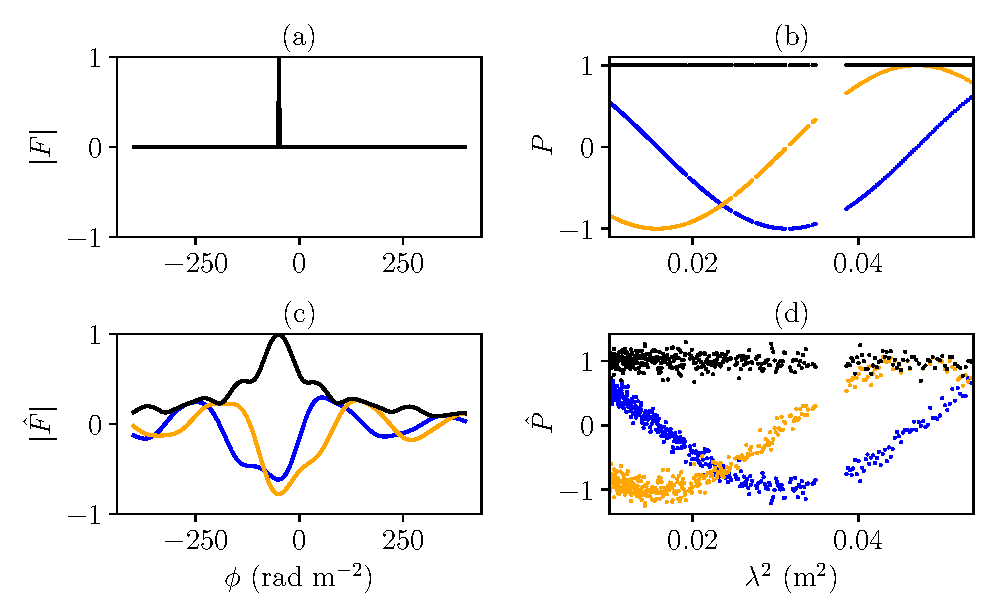
\includegraphics[width=\linewidth]{faraday-images/spectra_simple.pdf}
      \caption{A simple FDF and its corresponding polarised spectra: (a) groundtruth FDF $F$, (b) noise-free polarised spectrum $P$, (c) noisy observed FDF $\hat F$, (d) noisy polarised spectrum $\hat P$. Blue and orange mark real and imaginary components respectively.}
      \label{fig:simple-fdf}
    \end{figure}

    \begin{figure}
      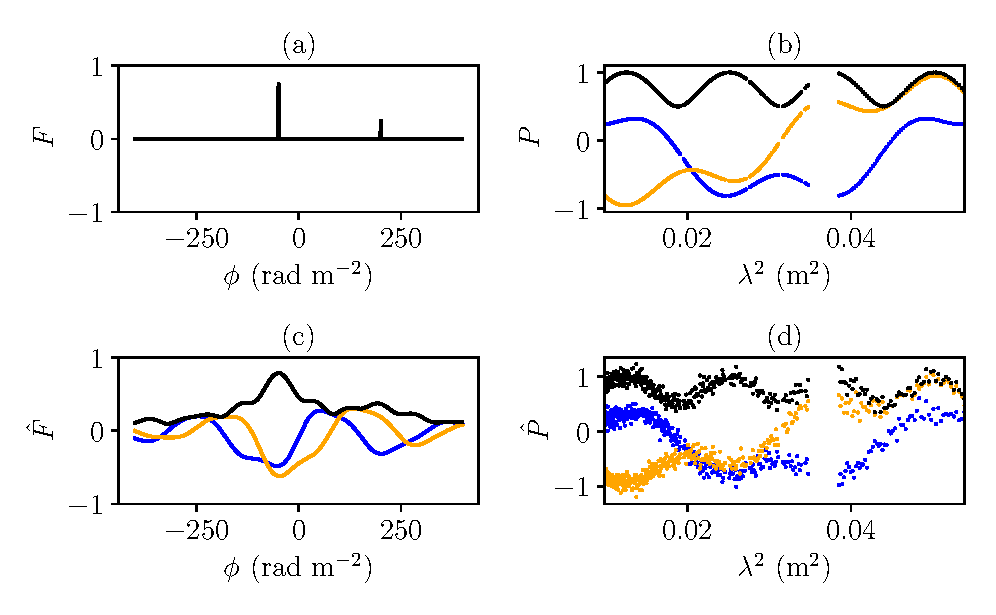
\includegraphics[width=\linewidth]{faraday-images/spectra.pdf}
      \caption{A complex FDF and its corresponding polarised spectra: (a) groundtruth FDF $F$, (b) noise-free polarised spectrum $P$, (c) noisy observed FDF $\hat F$, (d) noisy polarised spectrum $\hat P$. Blue and orange mark real and imaginary components respectively.}
      \label{fig:complex-fdf}
    \end{figure}

    Before we can classify FDFs as Faraday complex or Faraday simple, we need to define FDFs and any assumptions we make about them. An FDF is a function that maps Faraday depth $\phi$ to complex polarisation. It is the distribution of Faraday depths in an observed polarisation spectrum. For a given observation, we assume there is a true, noise-free FDF $F$ composed of at most two Faraday screens. This accounts for most actual sources \citep{anderson_broadband_2015} and extension to three screens would cover most of the remainder---\citet{osullivan_broad-band_2017} found that 89 per cent of their sources were best explained by two or less screens, while the remainder were best explained by three screens. We model the screens by Dirac delta distributions:
    \begin{equation}
        \label{eq:faraday-true-fdf}
        F(\phi) = A_0 \delta(\phi - \phi_0) + A_1 \delta(\phi - \phi_1).
    \end{equation}
    $A_0$ and $A_1$ are the polarised flux of each Faraday screen, and $\phi_0$ and $\phi_1$ are the Faraday depths of the respective screens. With this model, a Faraday simple source is one which has $A_0 = 0$, $A_1 = 0$, or $\phi_0 = \phi_1$. By using delta distributions to model each screen, we are assuming that there is no internal Faraday dispersion (which is typically associated with diffuse emission rather than the mostly-compact sources we expect to find in wide-area polarised surveys). $F$ generates a polarised spectrum of the form shown in \autoref{eq:faraday-true-pol}:
    \begin{equation}
        \label{eq:faraday-true-pol}
        P(\lambda^2) = A_0 e^{2i\phi_0\lambda^2} + A_1 e^{2i\phi_1\lambda^2}.
    \end{equation}
    Such a spectrum would be observed as noisy samples from a number of squared wavelengths $\lambda^2_j, j \in [1, \dots, D]$. We model this noise as a complex Gaussian with standard deviation $\sigma$ and call the noisy observed spectrum $\hat P$:
    \begin{equation}
      \label{eq:faraday-noisy-pol}
      \hat P(\lambda_j^2) \sim \mathcal N(P(\lambda^2_j), \sigma^2).
    \end{equation}
    The constant variance of the noise is a simplifying assumption which may not hold for real data, and exploring this is a topic for future work. By performing RM synthesis \citep{brentjens_faraday_2005} on $\hat P$ with uniform weighting we arrive at an observed FDF:
    \begin{equation}
      \label{eq:faraday-rm-synthesis}
      \hat F(\phi) = \frac{1}{D} \sum_{j = 1}^D \hat P(\lambda^2_j) e^{-2i\phi\lambda^2_j}.
    \end{equation}
    Examples of $F$, $\hat F$, $P$, and $\hat P$ for simple and complex observations are shown in \autoref{fig:simple-fdf} and \autoref{fig:complex-fdf} respectively. Note that there are two reasons that the observed FDF $\hat F$ does not match the groundtruth FDF $F$. The first is the noise in $\hat P$. The second arises from the incomplete sampling of $\hat P$.

    We do not consider external or internal Faraday dispersion in this work. External Faraday dispersion would broaden the delta functions of \autoref{eq:faraday-true-fdf} into peaks, and internal Faraday dispersion would broaden them into top-hat functions. All sources have at least a small amount of dispersion as the Faraday depth is a bulk property of the intervening medium and is subject to noise, but the assumption we make is that this dispersion is sufficiently small that the groundtruth FDFs are well-modelled with delta functions. Faraday thick sources would also invalidate our assumptions, and we assume that there are none in our data as Faraday thickness is hard to observe anyway \citeneeded{}. Nevertheless some external Faraday dispersion would be covered by our model, as depending on observing parameters Faraday thick sources may appear as two screens \citep{vaneck17faraday}.

    To simulate observed FDFs we follow the method of \citet{brown_classifying_2018}, which we describe in \autoref{sec:faraday-simulating}.

\section{Classification approach}
\label{sec:faraday-approach}

  The Faraday complexity classification problem is as follows: Given an FDF $\hat F$, is it Faraday complex or Faraday simple? In this section we describe the features that we have developed to address this problem, which can be used in any standard machine learning classifier. We trained two classifiers on these features, which we describe here also.

  \subsection{Features}
  \label{sec:faraday-scores-method}

    Our features are based on a simple idea: all simple FDFs look essentially the same, up to scaling and translation, while complex FDFs may deviate. A noise-free peak-normalised simple FDF $\hat F_{\mathrm{simple}}$ has the form
    \begin{align}
        \label{eq:faraday-f-simple}
        \hat F_{\mathrm{simple}}(\phi; \phi_s) &= R(\phi - \phi_s).
    \end{align}
    $\phi_s$ traces out a curve in the space of all possible FDFs. In other words, $\hat F_{\mathrm{simple}}$ is a manifold parametrised by $\phi_s$. Our features are derived from relating an observed FDF to the manifold of simple FDFs (the `simple manifold'). We can characterise an FDF by its distance to the simple manifold using some distance measure $D_f$:
    \begin{equation}
        \label{eq:faraday-complexity-model}
        \varsigma_f(\hat F) = \min_{\phi_s \in \mathbb{R}} D_f\infdivx{\hat F(\phi)}{\hat F_{\mathrm{simple}}(\phi; \phi_s)}.
    \end{equation}
    This distance has nice properties, as it is:
    \begin{itemize}
        \item invariant over changes in complex phase,
        \item translationally invariant in Faraday depth,
        \item zero for Faraday simple sources (i.e. when $A_0 = 0$, $A_1 = 0$, or $\phi_0 = \phi_1$) when there is no noise,
        \item symmetric in components (i.e. swapping $A_0 \leftrightarrow A_1$ and $\phi_0 \leftrightarrow \phi_1$ should not change the distance),
        \item increasing as $A_0$ and $A_1$ become closer to each other, and
        \item increasing as screen separation $|\phi_0 - \phi_1|$ increases over a large range.
    \end{itemize}
    Our features are constructed from this distance and its minimiser. In other words
    we look for the simple FDF $\hat{F}_{\mathrm{simple}}$ that is ``closest'' to the observed FDF $\hat{F}$.
    The minimiser $\phi_s$ is the Faraday depth of the simple FDF.

    While we could choose any distance that operates on functions, we used the 2-Wasserstein ($W_2$) distance \eqref{eq:faraday-W2-distance} and the Euclidean distance \eqref{eq:faraday-Euclidean-distance}. The $W_2$ distance operates on probability distributions and can be thought of as the minimum cost to `move' one probability distribution to the other, where the cost of moving one unit of probability mass is the squared distance it is moved. Under $W_2$ distance, the minimiser $\phi_w$ in \autoref{eq:faraday-complexity-model} can be interpreted as the Faraday depth that the FDF $\hat F$ would be observed to have if its complexity was unresolved (i.e. the weighted mean of its components). The Euclidean distance is the square root of the least-squares loss which is often used for fitting $\hat{F}_{\mathrm{simple}}$ to the FDF $\hat F$. Under Euclidean distance, the minimiser $\phi_s$ is equivalent to the depth of the best-fitting single component under assumption of Gaussian noise in $\hat F$.
    We calculated the $W_2$ distance using \texttt{Python Optimal Transport} \citep{flamary17pot}, and we calculated the Euclidean distance using \texttt{scipy.spatial.distance.euclidean} \citep{scipy2020}.
    Further intuition about the two distances is provided in \autoref{sec:faraday-interpreting-distances}.

    We denote by $\phi_w$ and $\phi_e$, the Faraday depth of the simple FDF that minimises the respective distances
    (2-Wasserstein and Euclidean).
    \begin{align*}
       \phi_w &= \underset{\phi_w}{\mathrm{argmin}}\ D_{W_2}\infdivx{\hat F(\phi)}{\hat F_{\mathrm{simple}}(\phi; \phi_w)},\\
       \phi_e &= \underset{\phi_e}{\mathrm{argmin}}\ D_E\infdivx{\hat F(\phi)}{\hat F_{\mathrm{simple}}(\phi; \phi_e)}.
     \end{align*}
     These features are depicted on an example FDF in \autoref{fig:features-on-fdf}.
     For simple observed FDFs, the fitted Faraday depths $\phi_w$ and $\phi_e$ both tend to be
     close to the peak of the observed FDF. However for complex observed FDFs, $\phi_w$ tends
     to be at the average depth between the two major peaks of the observed FDF, being closer
     to the higher peak. For notation convenience, we denote the Faraday depth of the
     observed FDF that has largest magnitude as $\phi_a$, i.e.
     \begin{equation*}
       \phi_a = \underset{\phi_a}{\mathrm{argmax}}\ |\hat F(\phi_a)|,\\
     \end{equation*}
     Note that in practice $\phi_a \approx \phi_e$.
     For complex observed FDFs, the values of Faraday depths $\phi_w$ and $\phi_a$ tend
     to differ (essentially by a proportion of the location of the second screen).
     The difference between $\phi_w$ and $\phi_a$ therefore provides useful information
     to identify complex FDFs.
     When the observed FDF is simple, the 2-Wasserstein fit will overlap significantly,
     hence the observed magnitudes $\hat F(\phi_w)$ and $\hat F(\phi_a)$ will be similar.
     However, for complex FDFs $\phi_w$ and $\phi_a$ are at different depths,
     leading to different values of $\hat F(\phi_w)$ and $\hat F(\phi_a)$.
     Therefore the magnitudes of the observed FDFs at the depths $\phi_w$ and $\phi_a$
     indicate how different the observed FDF is from a simple FDF.

    \begin{figure}
      \centering
      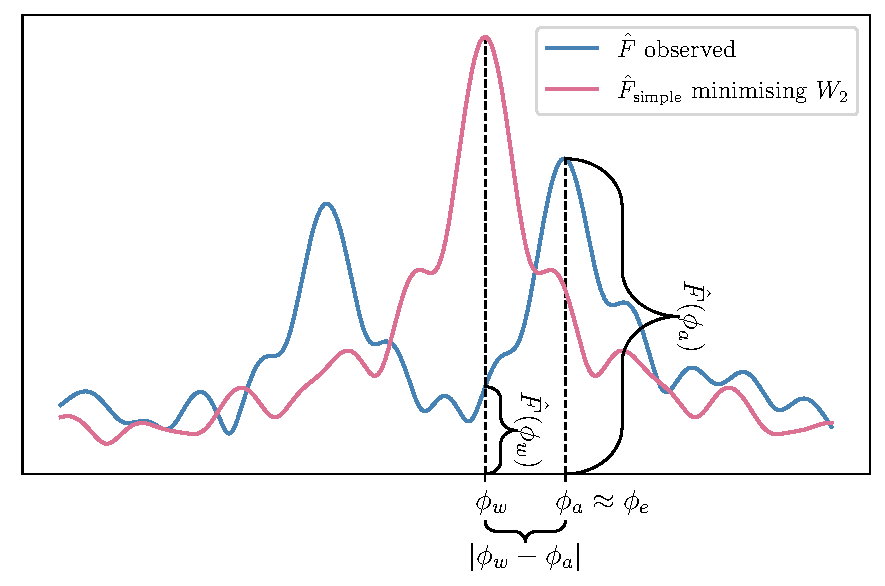
\includegraphics[width=\linewidth]{faraday-images/features_on_graph.pdf}
      \caption{\label{fig:features-on-fdf} An example of how an observed FDF $\hat F$ relates to our features. $\phi_w$ is the $W_2$-minimising Faraday depth, and $\phi_a$ is the $\hat F$-maximising Faraday depth (approximately equal to the Euclidean-minimising Faraday depth). The remaining two features are the $W_2$ and Euclidean distances between the depicted FDFs.}
    \end{figure}

    In summary, we provide the following features to the classifier:
    \begin{itemize}
      \item $\log |\phi_w - \phi_a|$,
      \item $\log \hat F(\phi_w)$,
      \item $\log \hat F(\phi_a)$,
      \item $\log D_{W_2}\infdivx{\hat F(\phi)}{\hat F_{\mathrm{simple}}(\phi; \phi_w)}$,
      \item $\log D_{E}\infdivx{\hat F(\phi)}{\hat F_{\mathrm{simple}}(\phi; \phi_e)}$,
    \end{itemize}
    where $D_E$ is the Euclidean distance, $D_{W_2}$ is the $W_2$ distance, $\phi_a$ is the Faraday depth of the FDF peak, $\phi_w$ is the minimiser for $W_2$ distance, and $\phi_e$ is the minimiser for Euclidean distance.

    \subsection{Interpreting distances}
    \label{sec:faraday-interpreting-distances}

    Interestingly, in the case where there is no RMSF, \autoref{eq:faraday-complexity-model} with $W_2$ distance reduces to the Faraday moment already in common use:
    \begin{align}
        D_{W_2}(F) &= \min_{\phi_w \in \mathbb{R}} D_{W_2}\infdivx{F(\phi)}{F_{\mathrm{simple}}(\phi; \phi_w)}\label{eq:faraday-W2-distance}\\
            &= \left(\frac{A_0A_1}{(A_0 + A_1)^2} (\phi_0 - \phi_1)^2\right)^{1/2}.
    \end{align}
    See \autoref{sec:faraday-w2-to-faraday-moments} for the corresponding calculation. In this sense, the $W_2$ distance can be thought of as a generalised Faraday moment, and conversely an interpretation of Faraday moments as a distance from the simple manifold in the case where there is no RMSF. Euclidean distance behaves quite differently in this case, and the resulting distance measure is totally independent of Faraday depth:
    \begin{align}
        D_{E}(F) &= \min_{\phi_e \in \mathbb{R}} D_E\infdivx{F(\phi)}{F_{\mathrm{simple}}(\phi; \phi_e)}\label{eq:faraday-Euclidean-distance}\\
            &= \sqrt{2} \frac{\min(A_0, A_1)}{A_0 + A_1}.
    \end{align}
    See \autoref{sec:faraday-euclidean-calculation} for the corresponding calculation.


  \subsection{Classifiers}
  \label{sec:faraday-classifiers}

    We trained two classifiers on simulated observations using these features: logistic regression (LR) and extreme gradient boosted trees (XGB). These classifiers are useful together for understanding Faraday complexity classification. LR is a linear classifier that is readily interpretable by examining the weights it applies to each feature. XGB is a powerful off-the-shelf non-linear ensemble classifier. We used the \texttt{scikit-learn} implementation of LR and we use the \texttt{XGBoost} library for XGB. We optimised hyperparameters for XGB using a fork of \texttt{xgboost-tuner} \footnote{\url{https://github.com/chengsoonong/xgboost-tuner}} as utilised by \citet{zhu20mutagenic}. We used 1~000 iterations of randomised parameter tuning and the hyperparameters we found are tabulated in \autoref{tab:hyperparameters-xgb}. We optimised hyperparameters for LR using a 5-fold cross-validation grid search implemented in \texttt{sklearn.model\textunderscore{}selection.GridSearchCV}. The resulting hyperparameters are tabulated in \autoref{tab:hyperparameters-lr}.

\section{Experimental method and results}
\label{sec:faraday-experiment-classification}

  We applied our classifiers to classify simulated (\autoref{sec:faraday-cnn-comparison} and \ref{sec:results-simulated}) and real (\autoref{sec:faraday-results-observed}) FDFs. We replicated the experimental setup of \citet{brown_classifying_2018} for comparison with the state-of-the-art CNN classification method, and we also applied our method to 142 real FDFs observed with the Australia Telescope Compact Array (ATCA) from Livingston et al. (in prep.) and \citet{osullivan_broad-band_2017}.

  \subsection{Data}

  \subsubsection{Simulated training and validation data}
  \label{sec:faraday-simulated-training-data}

    Our classifiers were trained and validated on simulated FDFs. We produced two sets of simulated FDFs, one for comparison with the state-of-the-art method in the literature and one for application to our observed FDFs (described in \autoref{sec:faraday-observational-data}). We refer to the former as the `ASKAP' dataset as it uses frequencies from the Australian Square Kilometre Array Pathfinder 12-antenna early science configuration. These frequencies included 900 channels from 700--1300 and 1500--1800~MHz and were used to generate simulated training and validation data by \citet{brown_classifying_2018}. We refer to the latter as the `ATCA' dataset as it uses frequencies from the 1--3~GHz configuration of the ATCA. These frequencies included 394 channels from 1.29--3.02~GHz and match our real data. We simulated Faraday depths from $-50$ to $50$ rad~m$^{-2}$ for the `ASKAP' dataset (matching Brown) and $-500$ to $500$ for the `ATCA' dataset.

    For each dataset, we simulated 100~000 FDFs, approximately half simple and half complex. We randomly allocated half of these FDFs to a training set and reserved the remaining half for validation. Each FDF had complex Gaussian noise added to the corresponding polarisation spectrum. For the `ASKAP' dataset, we sampled the standard deviation of the noise uniformly between 0 and $\sigma_{\max} = 0.333$, matching the dataset of \citet{brown_classifying_2018}.
    For the `ATCA' dataset, we fit a log-normal distribution to the standard deviations of O'Sullivan's data \citep{osullivan_broad-band_2017} from which we sampled our values of $\sigma$:
    \begin{equation}
      \sigma \sim \frac{1}{0.63 \sqrt{2 \pi} \sigma} \exp \left(-\frac{\log\left(50 \sigma - 0.5\right)^2}{2 \times 0.63^2}\right)
    \end{equation}


  \subsubsection{Observational data}
  \label{sec:faraday-observational-data}

    We used two real datasets containing a total of 142 sources: 42 polarised spectra from Livingston et al. (in prep.) and 100 polarised spectra from \citet{osullivan_broad-band_2017}. These datasets were observed in similar frequency ranges on the same telescope (with different binning), but are in different parts of the sky. The Livingston data were taken near the Galactic Centre, and the O'Sullivan data were taken away from the plane of the Galaxy. There are more Faraday complex sources near the Galactic Centre compared to more Faraday simple sources away from the plane of the Galaxy (Livingston et al.). The similar frequency channels used in the two datasets result in almost identical RMSFs over the Faraday depth range we considered (-500 to 500 rad m$^{-2}$), so we expected that the classifiers would work equally well on both datasets with no need to re-train. We discarded the 26 Livingston sources with modelled Faraday depths outside of this Faraday depth range, which we do not expect to affect the applicability of our methods to wide-area surveys because these fairly high depths are not common.

    Livingston et al. (in prep) used RM-CLEAN \citep{heald09faraday} to identify significant components in their FDFs. Some of these components had very high Faraday depths up to 2000 rad m$^{-2}$, but we chose to ignore these components in this chapter as they are much larger than might be expected in a wide-area survey like POSSUM. They used the second Faraday moment \citep{Brown11report} to estimate Faraday complexity, with Faraday depths determined using \texttt{scipy.signal.find\textunderscore{}peaks} on the cleaned FDFs, with a cutoff of 7 times the noise of the polarised spectrum. Using this method, they estimated that 89 per cent of their sources were Faraday complex i.e. had a Faraday moment greater than 0.

    \citet{osullivan_broad-band_2017} used the QU-fitting and model selection technique described in \citet{osullivan12agn}. The QU-fitting models contained up to three Faraday screen components as well as a term for internal and external Faraday dispersion. We ignore the Faraday thickness and dispersion for the purposes of this chapter, as most sources were not found to have Faraday thickness and dispersion is beyond the scope of our current work. 37 sources had just one component, 52 had two, and the remaining 11 had three.

  \subsection{Results on ``ASKAP'' dataset}
  \label{sec:faraday-cnn-comparison}

    The accuracy of the LR and XGB classifiers on the ``ASKAP'' testing set was 94.4 and 95.1 per cent respectively. The confusion matrices are shown in \autoref{tab:cm-lr-askap12} and \autoref{tab:cm-xgb-askap12}. These results are very close to the CNN presented by \citet{brown_classifying_2018}, with a slightly higher true negative rate and a slightly lower true positive rate (recalling that positive sources are complex, and negative sources are simple). The accuracy of the CNN was 94.9, slightly lower than our XGB classifier and slightly higher than our LR classifier. Both of our classifiers therefore produce similar classification performance to the CNN, with faster training time and easier interpretation.

  \subsection{Results on ``ATCA'' dataset}
  \label{sec:faraday-results-simulated}

    The accuracy of the LR and XGB classifiers on the ``ATCA'' dataset was 89.2 and 90.5 per cent respectively. The major differences between the ``ATCA'' and the ``ASKAP'' experiments are the range of the simulated Faraday depths and the distribution of noise levels. The ``ASKAP'' dataset, to match past CNN work, only included depths from $-50$ to $50$ rad m$^{-2}$, while the ``ATCA'' dataset includes depths from $-500$ to $500$ rad m$^{-2}$. The confusion matrices are shown in \autoref{tab:cm-lr} and \autoref{tab:cm-xgb}.

    \begin{figure}
      \begin{subfigure}{\linewidth}
        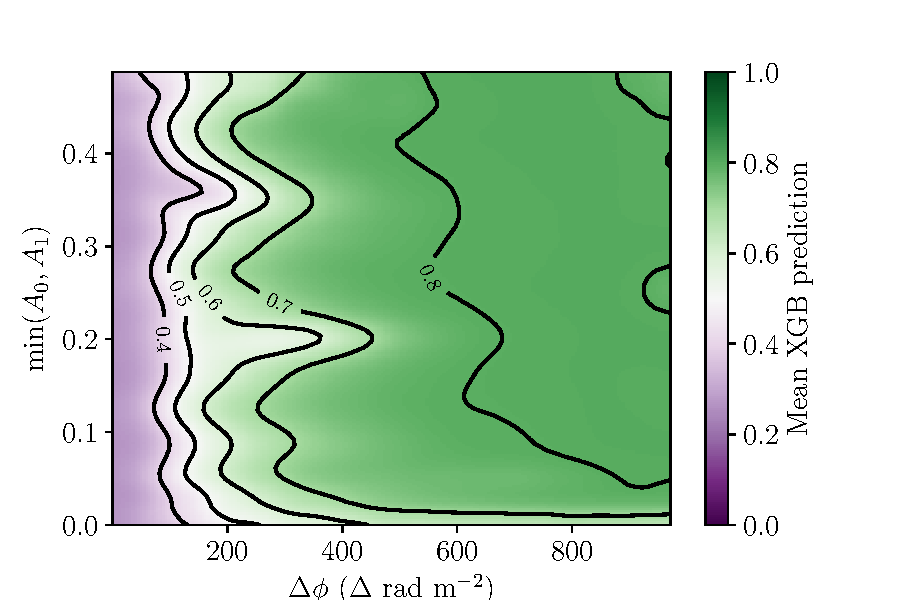
\includegraphics[width=\linewidth]{faraday-images/mean_xgb_prediction_dphi_amp.pdf}
        \caption{\label{fig:mean-xgb-pred}}
      \end{subfigure}
      \begin{subfigure}{\linewidth}
        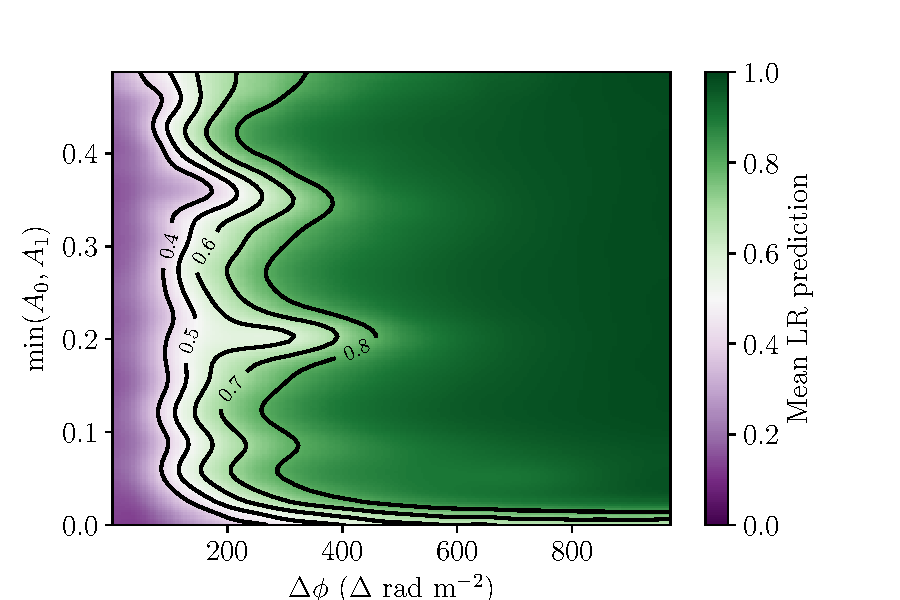
\includegraphics[width=\linewidth]{faraday-images/mean_lr_prediction_dphi_amp.pdf}
        \caption{\label{fig:mean-lr-pred}}
      \end{subfigure}
      \caption{\label{fig:amps-dphi-mean} Mean prediction as a function of component depth separation and minimum component amplitude for (a) XGB and (b) LR.}
    \end{figure}

    As we know the true Faraday depths of the components in our simulation, we can investigate the behaviour of these classifiers as a function of physical properties. \autoref{fig:amps-dphi-mean} shows the mean classifier prediction as a function of component depth separation and minimum component amplitude. This is tightly related to the mean accuracy, as the entire plot domain contains complex spectra besides the left and bottom edge: by setting the threshold to a value on this plot, the accuracy will be one hundred per cent on the non-edge for all higher values.

  \subsection{Results on observed FDFs}
  \label{sec:faraday-results-observed}

    % \begin{figure*}
    %   \centering
    %   \begin{subfigure}{0.45\linewidth}
    %     \includegraphics[width=\linewidth]{faraday-images/livingston_false_positive.pdf}
    %     \caption{Predicted complex.}
    %     \label{fig:livingston-false-positive}
    %   \end{subfigure}%
    %   \begin{subfigure}{0.45\linewidth}
    %     \includegraphics[width=\linewidth]{faraday-images/livingston_false_negative.pdf}
    %     \caption{Predicted simple.}
    %     \label{fig:livingston-false-negative}
    %   \end{subfigure}
    %   \begin{subfigure}{0.45\linewidth}
    %     \includegraphics[width=\linewidth]{faraday-images/osullivan_false_positive.pdf}
    %     \caption{Predicted complex.}
    %   \end{subfigure}%
    %   \begin{subfigure}{0.45\linewidth}
    %     \includegraphics[width=\linewidth]{faraday-images/osullivan_false_negative.pdf}
    %     \caption{Predicted simple.}
    %   \end{subfigure}
    %   \caption{Randomly-selected misclassified FDFs. (a) and (b) are from the Livingston dataset, and (c) and (d) are from the O'Sullivan dataset. (a) and (c) were misclassified as complex while (b) and (d) were misclassified as simple.}
    %   \label{fig:misclassified}
    % \end{figure*}

    \begin{figure*}
      \centering
      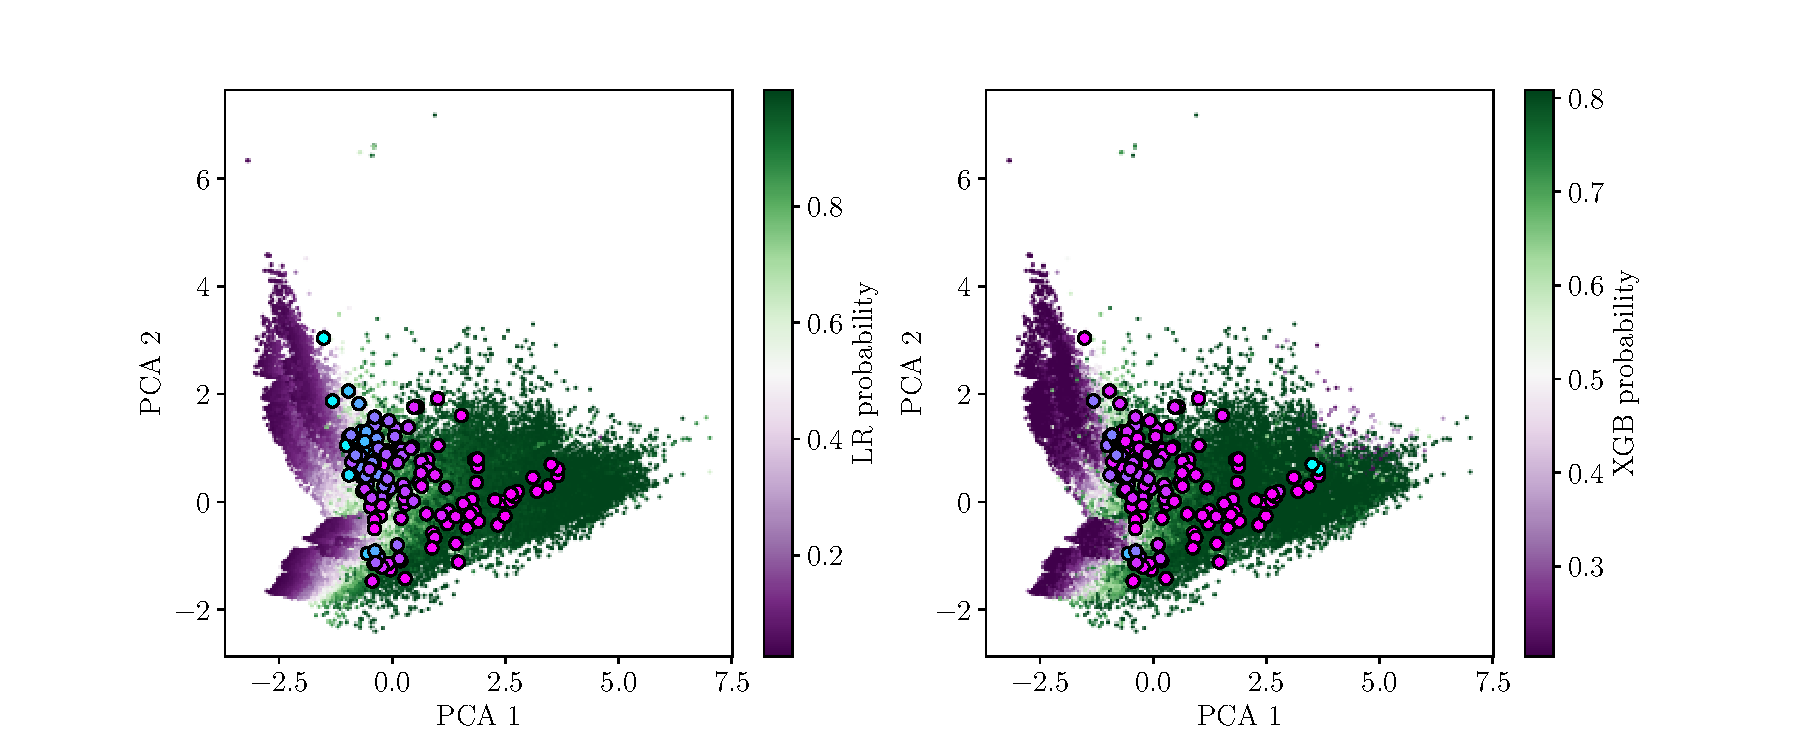
\includegraphics[width=\linewidth]{faraday-images/pca_with_overlay.pdf}
      \caption{Principal component analysis for simulated data (coloured dots) with observations overlaid (black-edged circles). Observations are coloured by their XGB or LR estimated probability of being complex, with blue indicating `most simple' and pink indicating `most complex'.}
      \label{fig:pca}
    \end{figure*}
    \begin{figure}
      \centering
      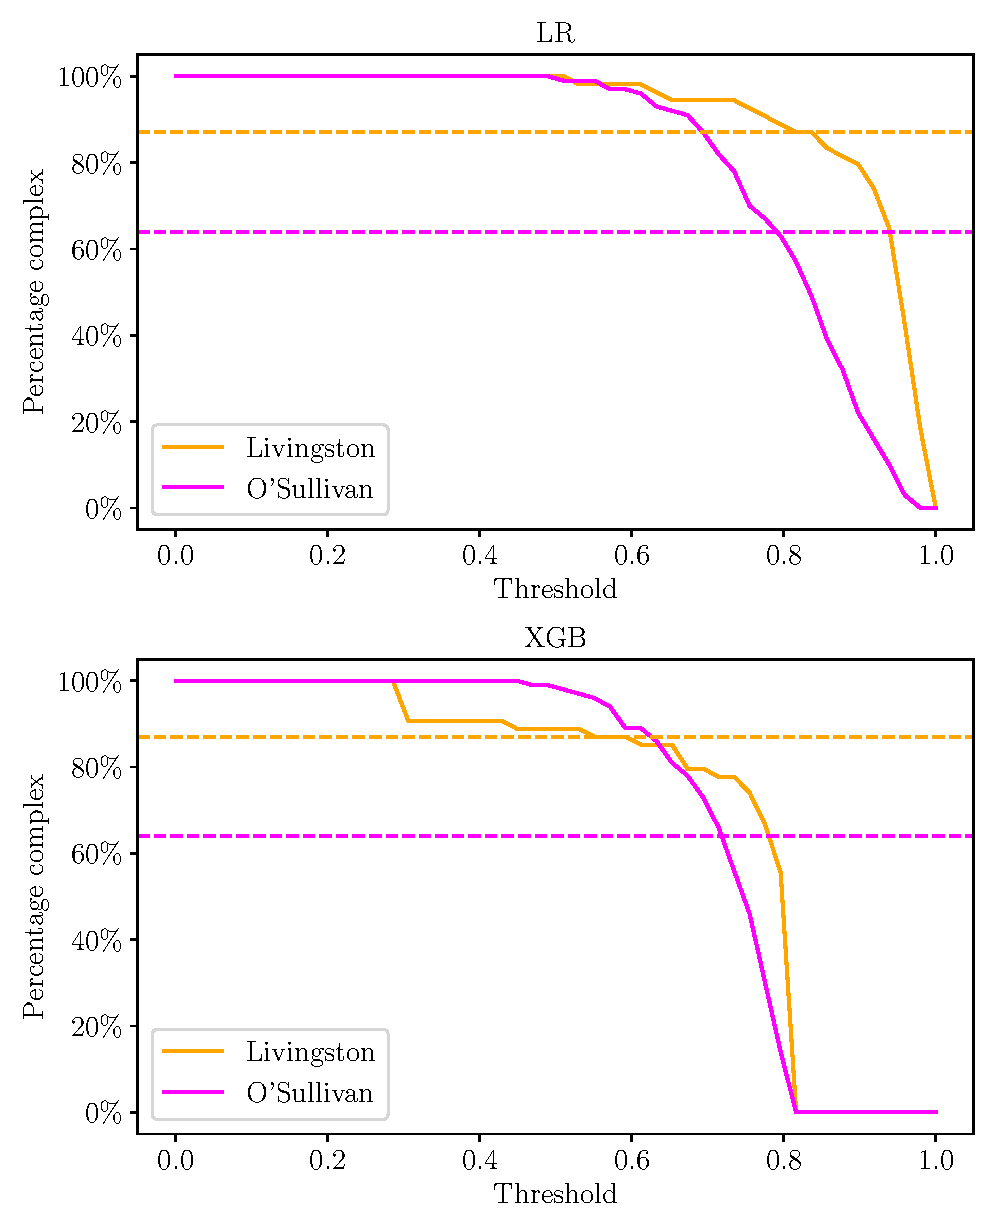
\includegraphics[width=\linewidth]{faraday-images/pc_complex_curves.pdf}
      \caption{Estimated rates of Faraday complexity for the Livingstone and O'Sullivan datasets as functions of threshold. The horizontal lines indicate the rates of Faraday complexity estimated by Livingston and O'Sullivan respectively.}
      \label{fig:complexity-rates}
    \end{figure}

    We used the LR and XGB classifiers which were trained on the ATCA simulation to estimate the probability that our 142 observed FDFs (\autoref{sec:faraday-observational-data}) were Faraday complex. As these classifiers were trained on simulated data, they face the issue of the `domain gap': the distribution of samples from a simulation differs from the distribution of real sources, and this affects performance on real data. Solving this issue is called `domain adaptation' and how to do this is an open research question in machine learning \citep{zhang2019transfer,pan10transfer}. Nevertheless, the features of our observations mostly fall in the same region of feature space as the simulations (\autoref{fig:pca}) and so we expect reasonably good domain transfer.

    Two apparently complex sources in the Livingston sample are classified as simple with high probability by XGB. These outliers are on the very edge of the training sample (\autoref{fig:pca}) and the underdensity of training data here is likely the cause of this issue. LR does not suffer the same issue, producing plausible predictions for the entire dataset, and these sources are instead classified as complex with high probability.

    With a threshold of 0.5, LR predicted that 96 and 83 per cent of the Livingston and O'Sullivan sources were complex respectively. This is in line with expectations that the Livingston data should have more Faraday complex sources than the O'Sullivan data due to their location near the Galactic Centre. XGB predicted that 93 and 100 per cent of the Livingston and O'Sullivan sources were complex respectively. Livingston et al. (in prep) found that 90 per cent of their sources were complex, and \citet{osullivan_broad-band_2017} found that 64 per cent of their sources were complex. This suggests that our classifiers are overestimating complexity, though it could also be the case that the methods used by Livingston and O'Sullivan underestimate complexity. Modifying the prediction threshold from 0.5 changes the estimated rate of Faraday complexity, and we show the estimated rates against threshold for both classifiers in \autoref{fig:complexity-rates}. We suggest that this result is indicative of our probabilities being uncalibrated, and a higher threshold should be chosen in practice. We chose to keep the threshold at 0.5 as this had the highest accuracy on the simulated validation data. The very high complexity rates of XGB and two outlying classifications indicate that the XGB classifier may be overfitting to the simulation and that it is unable to generalise across the domain gap.

    \autoref{fig:all-observed-fdfs-lr} and \autoref{fig:all-observed-fdfs-xgb} show every observed FDF ordered by estimated Faraday complexity, alongside the models predicted by Livingston and O'Sullivan, for LR and XGB respectively. There is a clear visual trend of increasingly complex sources with increasing predicted probability of being complex. %The complex FDFs in the Livingston dataset that were identified as simple by the classifier tend to have very different component amplitudes and a very high signal-to-noise main peak, while the simple FDFs identified as complex tend to be very noisy.

\section{Discussion}
\label{sec:faraday-discussion}

  % \todo{Changing the bias of the classifiers would allow us to optimise for high precision or high recall depending on the use case of the classifier, but we optimised for maximum accuracy here.}

  On simulated data (\autoref{sec:faraday-results-simulated}) we achieve state-of-the-art accuracy. Our results on observed FDFs show that our classifiers produce plausible results, with \autoref{fig:all-observed-fdfs-lr} and \autoref{fig:all-observed-fdfs-xgb} showing a clear trend of apparent complexity. Some issues remain: we discuss the intrinsic overlap between simple and complex FDFs in \autoref{sec:faraday-overlap} and the limitations of our method in \autoref{sec:faraday-limitations}.

  % \subsection{Interpretable classification}

  %   Our classifiers are interpretable. The features are easy to understand and have clear relationship to the true simulation parameters, and the classifiers themselves are simple enough that it is possible to understand how the classifier came to a given classification for a given source. LR is particularly simple, and similar enough in performance to XGB that it may be the preferable classifier for Faraday complexity estimation. We can examine its weights to find why it predicted a given FDF was simple or complex. For example, in \autoref{fig:misclassified}, a) was classified as complex due to its low maximum value of $|\hat F|$ and its high Euclidean distance from the simple manifold, b) and d) were both classified as simple due to their low Euclidean distance from the simple manifold, and c) was classified as complex due to its high maximum $|\hat F|$ and $W_2$ distance from the simple manifold (though the prediction is very close to the decision boundary because it has a low Euclidean distance from the simple manifold). Interpretability in a classifier is valuable in astronomy, as understanding the limitations and behaviour of our methods is important to ensure that any physical predictions we make from our results are sensible, well-motivated, and consistent with physics.

  \subsection{Complexity and seeming `not simple'}
  \label{sec:faraday-overlap}

    Through this work we found our methods limited by the significant overlap between complex and simple FDFs. Complex FDFs can be consistent with simple FDFs due to close Faraday components or very small amplitudes on the secondary component, and vice versa due to noise.

    % \autoref{fig:livingston-false-negative} is an example of such a classification. Due to this effect we should expect a lower rate of complexity than the true complexity rate. We demonstrated this in \autoref{sec:faraday-results-observed} where our methods predict lower rates of Faraday complexity than the methods of Faraday moments and QU-fitting employed by Livingston and O'Sullivan respectively. Of course, issues like model overfitting (with QU-fitting) or high sensitivity to choice of noise cutoff (with RM-CLEAN and Faraday moments) may also inflate the rate of complexity in the O'Sullivan and Livingston models respectively, so we refrain from stating that either complexity estimation method is \emph{wrong}, just that they do not match. For any given source, both methods may produce plausible but disagreeing results.
    % Surely this is a good place to discuss the merits of being conservative in developing a catalog?  For example, an RM catalogue of high S/N sources could be easily derived with your classifier because it would be conservative to selecting simple sources

    The main failure mode of our classifiers is misclassifying a complex source as simple (\autoref{tab:cm-lr} and \autoref{tab:cm-xgb}). Whether sources with close components or small amplitudes should be considered complex is not clear, since for practical purposes they can be treated as simple: assuming the source is simple yields a very similar RM to the RM of the primary component, and thus would not negatively impact further data products such as an RM grid. The scenarios where we would want a Faraday complexity classifier rather than a polarisation structure model---large-scale analysis and wide-area surveys---do not seem to be disadvantaged by considering such sources simple. Additional sources similar to these are likely hidden in presumably `simple' FDFs by the frequency range and spacing of the observations, just as how these complex sources would be hidden in lower-resolution observations. Note also that misidentification of complex sources as simple is intrinsically a problem with complexity estimation even for models not well-represented by a simple FDF, as complex sources may conspire to appear as a wide range of viable models including simple \citep{sun15comparison}.

    Conversely, high-noise simple FDFs may be consistent with complex FDFs. One key question is how Faraday complexity estimators should behave as the noise increases: should high noise result in a complex prediction or a simple prediction, given that a complex or simple FDF would both be consistent with a noisy FDF? Occam's razor suggests that we should choose the simplest suitable model, and so increasing noise should lead to predictions of less complexity. This is not how our classifiers operate, however: high-noise FDFs are different to the model simple FDFs and so are predicted to be `not simple'. In some sense our classifiers are not looking for complex sources, but are rather looking for `not simple' sources.

  \subsection{Limitations}
  \label{sec:faraday-limitations}

    Our main limitations are our simplifying assumptions on FDFs and the domain gap between simulated and real observations.

    It is unclear what the effect of our simplifying assumptions are on the effectiveness of our simulation. The three main simplifications we think may negatively affect our simulations are 1) limiting to two components, 2) assuming no external Faraday dispersion, and 3) assuming no internal Faraday dispersion (Faraday thickness). Future work will explore removing these simplifying assumptions, but will need to account for the increased difficulty in characterising the simulation with more components and no longer having Faraday screens as components. Additionally, more work will be required to make sure that the rates of internal and external Faraday dispersion match what might be expected from real sources, or risk making a simulation that has too large a range of consistent models for a given source: for example, a two-component source could also be explained as a sufficiently wide or resolved-out Faraday thick source or a three-component source with a small third component. This greatly complicates the classification task.

    Previous machine learning work \citep[e.g.][]{brown_classifying_2018} has not been run before on real FDF data, so this chapter is the first example of the domain gap arising in Faraday complexity classification. This is a problem that requires further research to solve. We have no good way to ensure that our simulation matches reality, so some amount of domain adaptation will always be necessary to train classifiers on simulated data and then apply these classifiers to real data. But with the low source counts in polarisation science (high-resolution spectropolarimetric data currently numbers in the few hundreds) any machine learning method will need to be trained on simulations. This is not just a problem in Faraday complexity estimation, and domain adaptation is also an issue faced in the wider astroinformatics community: large quantities of labelled data are hard to come by, and some sources are very rare \citep[e.g. gravitational wave detections or fast radio bursts;][]{zevin17gravityspy, gebhard19convolutional, agarwal20fetch}. LR seems to handle the domain adaptation better than XGB, with only a slightly lower accuracy on simulated data. Our results are plausible and the distribution of our simulation well overlaps the distribution of our real data (\autoref{fig:pca}).

    % \autoref{fig:acc-noise} demonstrates that the accuracy of our classifiers is dependent on the amount of noise in the simulated FDF in a surprising way: the correlation between noise and accuracy is not monotonic, and instead accuracy \emph{increases} as the noise increases up to the mean noise level of the training set. The classifier is forced to generalise over different amounts of noise with no good way to estimate how much noise is in a given FDF. This could be remedied by including noise as a feature, as suggested by \autoref{fig:acc-noise-retrained} which shows improved classifier behaviour when the training set was divided into different amounts of noise and the classifier was only trained and validated on FDFs with similar amounts of noise. But this is hard to generalise to real data: we would need not only a reliable noise estimate, but a reliable noise estimate that behaves in the same way to the simulated noise. The mean noise of the Livingston data was $0.028_{-0.022}^{+0.024}$, much lower than our simulated noise. This, combined with the fact that our simulated FDFs look very similar to the observed FDFs, suggests that either or both a) the injected noise and real noise have different units, or b) important aspects of the observed data are not captured by our simulation. This is another example of the domain gap in action and further research is required to unify the simulated and observed noise. The amount of noise can then be included as a feature for the classifier, which could greatly improve performance on both simulated and observed data.

\section{Conclusion}
\label{sec:faraday-conclusion}

  We developed a simple, interpretable machine learning method for estimating Faraday complexity. Our interpretable features were derived by comparing observed FDFs to idealised simple FDFs, which we could determine both for simulated and real observations. We demonstrated the effectiveness of our method on both simulated and real data. Using simulated data, we found that our classifiers were 95 per cent accurate, with near perfect recall of Faraday simple sources (specificity). On simulated data that matched existing observations, our classifiers obtained an accuracy of 90 per cent. Evaluating our classifiers on real data gave plausible results. Future work will need to narrow the domain gap to improve transfer of classifiers trained on simulations to real, observed data.

  % If we were to run our classifiers at scale on the upcoming POSSUM survey, how would the limitations presented in \autoref{sec:faraday-results-simulated} affect derived statistics of Faraday complexity?

  % \begin{itemize}
  %   \item Mention Brown cuts. What are the implications for POSSUM if we were to use our classifier? How does this affect what we can detect and can't?
  % \end{itemize}

  % \begin{itemize}
  %   \item (10) is a good example of noise being important but we can't explicitly factor it in yet - this is two peaks that are very different scales
  %   \item (27) is funky, we get a smooth-looking FDF but it's not obviously two peaks. see also (47)
  %   \item (38) has $\phi_s$ outside of the range! but it still looks good
  % \end{itemize}


\appendix

  \section{2-Wasserstein begets Faraday moments}
  \label{sec:faraday-w2-to-faraday-moments}
    Minimising the 2-Wasserstein distance between a model FDF and the simple manifold gives the second Faraday moment of that FDF. Let $\tilde F$ be the sum-normalised model FDF and let $\tilde S$ be the sum-normalised simple model FDF:
    \begin{align}
      \tilde F(\phi) &= \frac{A_0 \delta(\phi - \phi_0) + A_1 \delta(\phi - \phi_1)}{A_0 + A_1}\\
      \tilde S(\phi; \phi_w) &= \delta(\phi - \phi_w).
    \end{align}
    The $W_2$ distance, usually defined on probability distributions, can be extended to one-dimensional complex functions $A$ and $B$ by normalising them:
      \begin{align}
        \label{eq:faraday-w2}
        D_{W_2}\infdivx{A}{B}^2 &= \inf_{\gamma \in \Gamma(A, B)} \iint_{\phi_{\min}}^{\phi_{\max}} |x - y|^2\ \mathrm{d}\gamma(x, y) \\
        \label{eq:faraday-normalised}
        \tilde A(\phi) &= \frac{|A(\phi)|}{\int_{\phi_{\min}}^{\phi_{\max}} |A(\theta)|\ \mathrm{d}\theta}\\
        \tilde B(\phi) &= \frac{|B(\phi)|}{\int_{\phi_{\min}}^{\phi_{\max}} |B(\theta)|\ \mathrm{d}\theta}
      \end{align}
      where $\Gamma(A, B)$ is the set of couplings of $A$ and $B$, i.e. the set of joint probability distributions that marginalise to $A$ and $B$; and $\inf_{\gamma \in \Gamma(A, B)}$ is the infimum over $\Gamma(A, B)$. This can be interpreted as the minimum cost to `move' one probability distribution to the other, where the cost of moving one unit of probability mass is the squared distance it is moved.

    The set of couplings $\Gamma(\tilde F, \tilde S)$ is the set of all joint probability distributions $\gamma$ such that
    \begin{align}
      \int_{\phi_{\min}}^{\phi_{\max}} \gamma(\phi, \varphi)\ \mathrm{d}\phi &= \tilde S(\varphi; \phi_w),\\
      \int_{\phi_{\min}}^{\phi_{\max}} \gamma(\phi, \varphi)\ \mathrm{d}\varphi &= \tilde F(\phi).
    \end{align}
    The coupling that minimises the integral in \autoref{eq:faraday-w2} will be the optimal transport plan between $\tilde F$ and $\tilde S$. Since $\tilde F$ and $\tilde S$ are defined in terms of delta functions, the optimal transport problem reduces to a discrete optimal transport problem and the optimal transport plan is:
    \begin{equation}
      \gamma(\phi, \varphi) = \frac{A_0 \delta(\phi - \phi_0) + A_1 \delta(\phi - \phi_1)}{A_0 + A_1} \delta(\varphi - \phi_w).
    \end{equation}
    In other words, to move the probability mass of $\tilde S$ to $\tilde F$, a fraction $A_0/(A_0 + A_1)$ is moved from $\phi_w$ to $\phi_0$ and the complementary fraction $A_1/(A_0 + A_1)$ is moved from $\phi_w$ to $\phi_1$. Then:
    \begin{align}
      D_{W_2}\infdivx{\tilde F}{\tilde S}^2 &= \iint_{\phi_{\min}}^{\phi_{\max}} |\phi - \varphi|^2\ \mathrm{d}\gamma(\phi, \varphi)\\
        % &= \frac{\iint_{\phi_{\min}}^{\phi_{\max}} (A_0 \delta(\phi - \phi_0) + A_1 \delta(\phi - \phi_1)) \delta(\varphi - \phi_w) (\phi - \varphi)^2\ \mathrm{d}\phi\ \mathrm{d}\varphi}{A_0 + A_1}\\
        % &= \frac{\int_{\phi_{\min}}^{\phi_{\max}} (A_0 \delta(\phi - \phi_0) + A_1 \delta(\phi - \phi_1)) (\phi - \phi_w)^2\ \mathrm{d}\phi}{A_0 + A_1}\\
        &= \frac{A_0 (\phi_0 - \phi_w)^2 + A_1 (\phi_1 - \phi_w)^2}{A_0 + A_1}.
    \end{align}
    To obtain the $W_2$ distance to the simple manifold, we need to minimise this over $\phi_w$. Differentiate with respect to $\phi_w$ and set equal to zero to find
    \begin{equation}
      \phi_w = \frac{A_0 \phi_0 + A_1 \phi_1}{A_0 + A_1}.
    \end{equation}
    Substituting this back in, we find
    \begin{align}
      \varsigma_{W_2}(F)^2 &= \frac{A_0 A_1}{A_0 + A_1}(\phi_0 - \phi_1)^2
    \end{align}
    which is the Faraday moment.

\section{Euclidean distance in the no-RMSF case}
\label{sec:faraday-euclidean-calculation}

  In this section we calculate the minimumised Euclidean distance evaluated on a model FDF (\autoref{eq:faraday-true-fdf}). Let $\tilde F$ be the sum-normalised model FDF and let $\tilde S$ be the normalised simple model FDF:
  \begin{align}
    \tilde F(\phi) &= \frac{A_0 \delta(\phi - \phi_0) + A_1 \delta(\phi - \phi_1)}{A_0 + A_1}\\
    \tilde S(\phi; \phi_e) &= \delta(\phi - \phi_e).
  \end{align}

  The Euclidean distance between $\tilde F$ and $\tilde S$ is then
  \begin{align}
    &D_E\infdivx{\tilde F(\phi)}{\tilde S(\phi; \phi_e)}^2\\
    &= \int_{\phi_{\min}}^{\phi_{\max}} \left|\tilde F(\phi) - \delta(\phi - \phi_e) \right|^2\ \mathrm{d}\phi.
  \end{align}

  Assume $\phi_0 \neq \phi_1$ (otherwise, $D_E$ will always be either $0$ or $2$). If $\phi_e = \phi_0$, then
  \begin{align}
    &D_E\infdivx{\tilde F(\phi)}{\tilde S(\phi; \phi_e)}^2\\
      &= \frac{1}{(A_0 + A_1)^2} \int_{\phi_{\min}}^{\phi_{\max}} A_1^2 \left|\delta(\phi - \phi_1) - \delta(\phi - \phi_0) \right|^2\ \mathrm{d}\phi\\
      &= \frac{2 A_1^2}{(A_0 + A_1)^2}
  \end{align}
  and similarly for $\phi_e = \phi_1$. If $\phi_e \neq \phi_0$ and $\phi_e \neq \phi_1$, then
  \begin{equation}
    D_E\infdivx{\tilde F(\phi)}{\tilde S(\phi; \phi_e)}^2 = \frac{A_0^2 + A_1^2 + 1}{(A_0 + A_1)^2}.
  \end{equation}
  The minimised Euclidean distance when $\phi_0 \neq \phi_1$ is therefore
  \begin{align}
      D_E(F) &= \min_{\phi_e \in \mathbb{R}} D_E\infdivx{F(\phi)}{F_{\mathrm{simple}}(\phi; \phi_e)}\\
          &= \sqrt{2} \frac{\min(A_0, A_1)}{A_0 + A_1}.
  \end{align}
  If $\phi_0 = \phi_1$, then the minimised Euclidean distance is 0.

% \section{Minimisation over simple FDFs}
% \label{sec:faraday-minimisation}

%   As part of our method, we need to minimise a divergence function $D_f$ over the manifold of simple FDFs $\hat F_{\mathrm{simple}}$:
%   \begin{equation}
%       \varsigma_f(\hat F) = \min_{\phi_w \in \mathbb{R}} D_f\infdivx{\hat F(\phi)}{\hat F_{\mathrm{simple}}(\phi; \phi_s)}.
%   \end{equation}
%   To do this, we perform a two-step approach. This two-step approach allows us to find a smooth (i.e. not discretised) minimum without encountering local minima due to the non-convexity of the optimisation target. First, we generate 1~000 noise-free simple FDFs using the same frequencies as those used to observe $\hat F$, with $\sigma = 0$ and $\phi_0 \in \{\phi_{\min}, \phi_{\min} + \delta\phi, \dots, \phi_{\max}\}$. This is a discrete representation of the simple manifold. We then evaluate $D_f$ between our observed FDF $\hat F$ and these simple spectra and identify the $\phi_0$ that gives us the smallest value of $D_f\infdivx{\hat F(\phi)}{\hat F_{\mathrm{simple}}(\phi; \phi_0)}$. Call this $\phi_0^{(1)}$. This gives us an initial guess at the minimising value of $\phi_s$ in \autoref{eq:faraday-complexity-model}. Second, we use \texttt{scipy.optimize.fmin\textunderscore{}bfgs} to minimise $D_f\infdivx{\hat F(\phi)}{\hat F_{\mathrm{simple}}(\phi; \phi_s)}$ over $\phi_s$ using $\phi_0^{(1)}$ as an initial value, producing a new minimiser $\phi_0^{(2)}$.

\section{Hyperparameters for LR and XGB}
\label{sec:faraday-hyperparameters}

  This section contains tables of the hyperparameters that we used for our classifiers. \autoref{tab:hyperparameters-xgb} and \autoref{tab:hyperparameters-lr} tabulate the hyperparameters for XGB and LR respectively for the ATCA dataset. \autoref{tab:hyperparameters-xgb-askap12} and \autoref{tab:hyperparameters-lr-askap12} tabulate the hyperparameters for XGB and LR respectively for the ASKAP dataset.

  \begin{table}
    \caption{\label{tab:hyperparameters-xgb} XGB hyperparameters for the ATCA dataset.}
    \begin{tabular}{ll}
      \hline\hline
      Parameter & Value\\\hline
      colsample\textunderscore{}bytree & 0.912\\
      gamma & 0.532\\
      learning\textunderscore{}rate & 0.1\\
      max\textunderscore{}depth & 7\\
      min\textunderscore{}child\textunderscore{}weight & 2\\
      scale\textunderscore{}pos\textunderscore{}weight & 1\\
      subsample & 0.557\\
      n\textunderscore{}estimators & 135\\
      reg\textunderscore{}alpha & 0.968\\
      reg\textunderscore{}lambda & 1.420\\
      \hline\hline
    \end{tabular}
  \end{table}

  \begin{table}
    \caption{\label{tab:hyperparameters-lr} LR hyperparameters for the ATCA dataset.}
    \begin{tabular}{ll}
      \hline\hline
      Parameter & Value\\\hline
      penalty & L1\\
      C & 1.668\\
      \hline\hline
    \end{tabular}
  \end{table}

  \begin{table}
    \caption{\label{tab:hyperparameters-xgb-askap12} XGB hyperparameters for the ASKAP dataset.}
    \begin{tabular}{ll}
      \hline\hline
      Parameter & Value\\\hline
      colsample\textunderscore{}bytree & 0.865\\
      gamma & 0.256\\
      learning\textunderscore{}rate & 0.1\\
      max\textunderscore{}depth & 6\\
      min\textunderscore{}child\textunderscore{}weight & 1\\
      scale\textunderscore{}pos\textunderscore{}weight & 1\\
      subsample & 0.819\\
      n\textunderscore{}estimators & 108\\
      reg\textunderscore{}alpha & 0.049\\
      reg\textunderscore{}lambda & 0.454\\
      \hline\hline
    \end{tabular}
  \end{table}

  \begin{table}
    \caption{\label{tab:hyperparameters-lr-askap12} LR hyperparameters for the ASKAP dataset.}
    \begin{tabular}{ll}
      \hline\hline
      Parameter & Value\\\hline
      penalty & L2\\
      C & 0.464\\
      \hline\hline
    \end{tabular}
  \end{table}

\section{Confusion matrices}
\label{sec:faraday-cms}

  This section contains confusion matrices for our classifiers evaluated on simulated ATCA and ASKAP data, as well as a confusion matrix from the state-of-the-art CNN classifier on simulated ASKAP data. \autoref{tab:cm-lr-askap12}, \autoref{tab:cm-lr-askap12}, and \autoref{tab:cm-brown} are confusion matrices on the ASKAP data for LR, XGB, and CNN respectively. \autoref{tab:cm-lr} and \autoref{tab:cm-xgb} are confusion matrices on the ATCA data for LR and XGB respectively.

    \begin{table}
      \caption{\label{tab:cm-lr-askap12} Logistic regression confusion matrix for the ASKAP simulation.}
      \begin{tabular}{r|cc}
        \hline\hline
        & Pred. simple & Pred. complex \\\hline
        True simple & 0.99 & 0.01 \\
        True complex & 0.10 & 0.90 \\
        \hline\hline
      \end{tabular}\\
      \\
      \caption{\label{tab:cm-xgb-askap12} XGB confusion matrix for the ASKAP simulation.}
      \begin{tabular}{r|cc}
        \hline\hline
        & Pred. simple & Pred. complex \\\hline
        True simple & 0.99 & 0.01 \\
        True complex & 0.09 & 0.91 \\
        \hline\hline
      \end{tabular}\\
      \\
      \caption{\label{tab:cm-brown} CNN confusion matrix for the ASKAP simulation, adapted from \citet{brown_classifying_2018}.}
      \begin{tabular}{r|cc}
        \hline\hline
        & Pred. simple & Pred. complex \\\hline
        True simple & 0.97 & 0.03 \\
        True complex & 0.07 & 0.93 \\
        \hline\hline
      \end{tabular}
    \end{table}

    \begin{table}
      \caption{\label{tab:cm-lr} Logistic regression confusion matrix for the ATCA dataset.}
      \begin{tabular}{r|cc}
        \hline\hline
        & Pred. simple & Pred. complex \\\hline
        True simple & 0.92 & 0.08 \\
        True complex & 0.16 & 0.84 \\
        \hline\hline
      \end{tabular}\\
      \\
      \caption{\label{tab:cm-xgb} XGB confusion matrix for the ATCA dataset.}
      \begin{tabular}{r|cc}
        \hline\hline
        & Pred. simple & Pred. complex \\\hline
        True simple & 0.91 & 0.09 \\
        True complex & 0.10 & 0.90 \\
        \hline\hline
      \end{tabular}
    \end{table}

\section{Predictions on real data}
\label{sec:faraday-real-data-fig}

  This section contains \autoref{fig:all-observed-fdfs-lr} and \autoref{fig:all-observed-fdfs-xgb}, which shows the predicted probability of being Faraday complex for all real data used in this chapter, drawn from Livingston et al. (in prep.) and \citet{osullivan_broad-band_2017}.

  \begin{figure*}
    \centering
    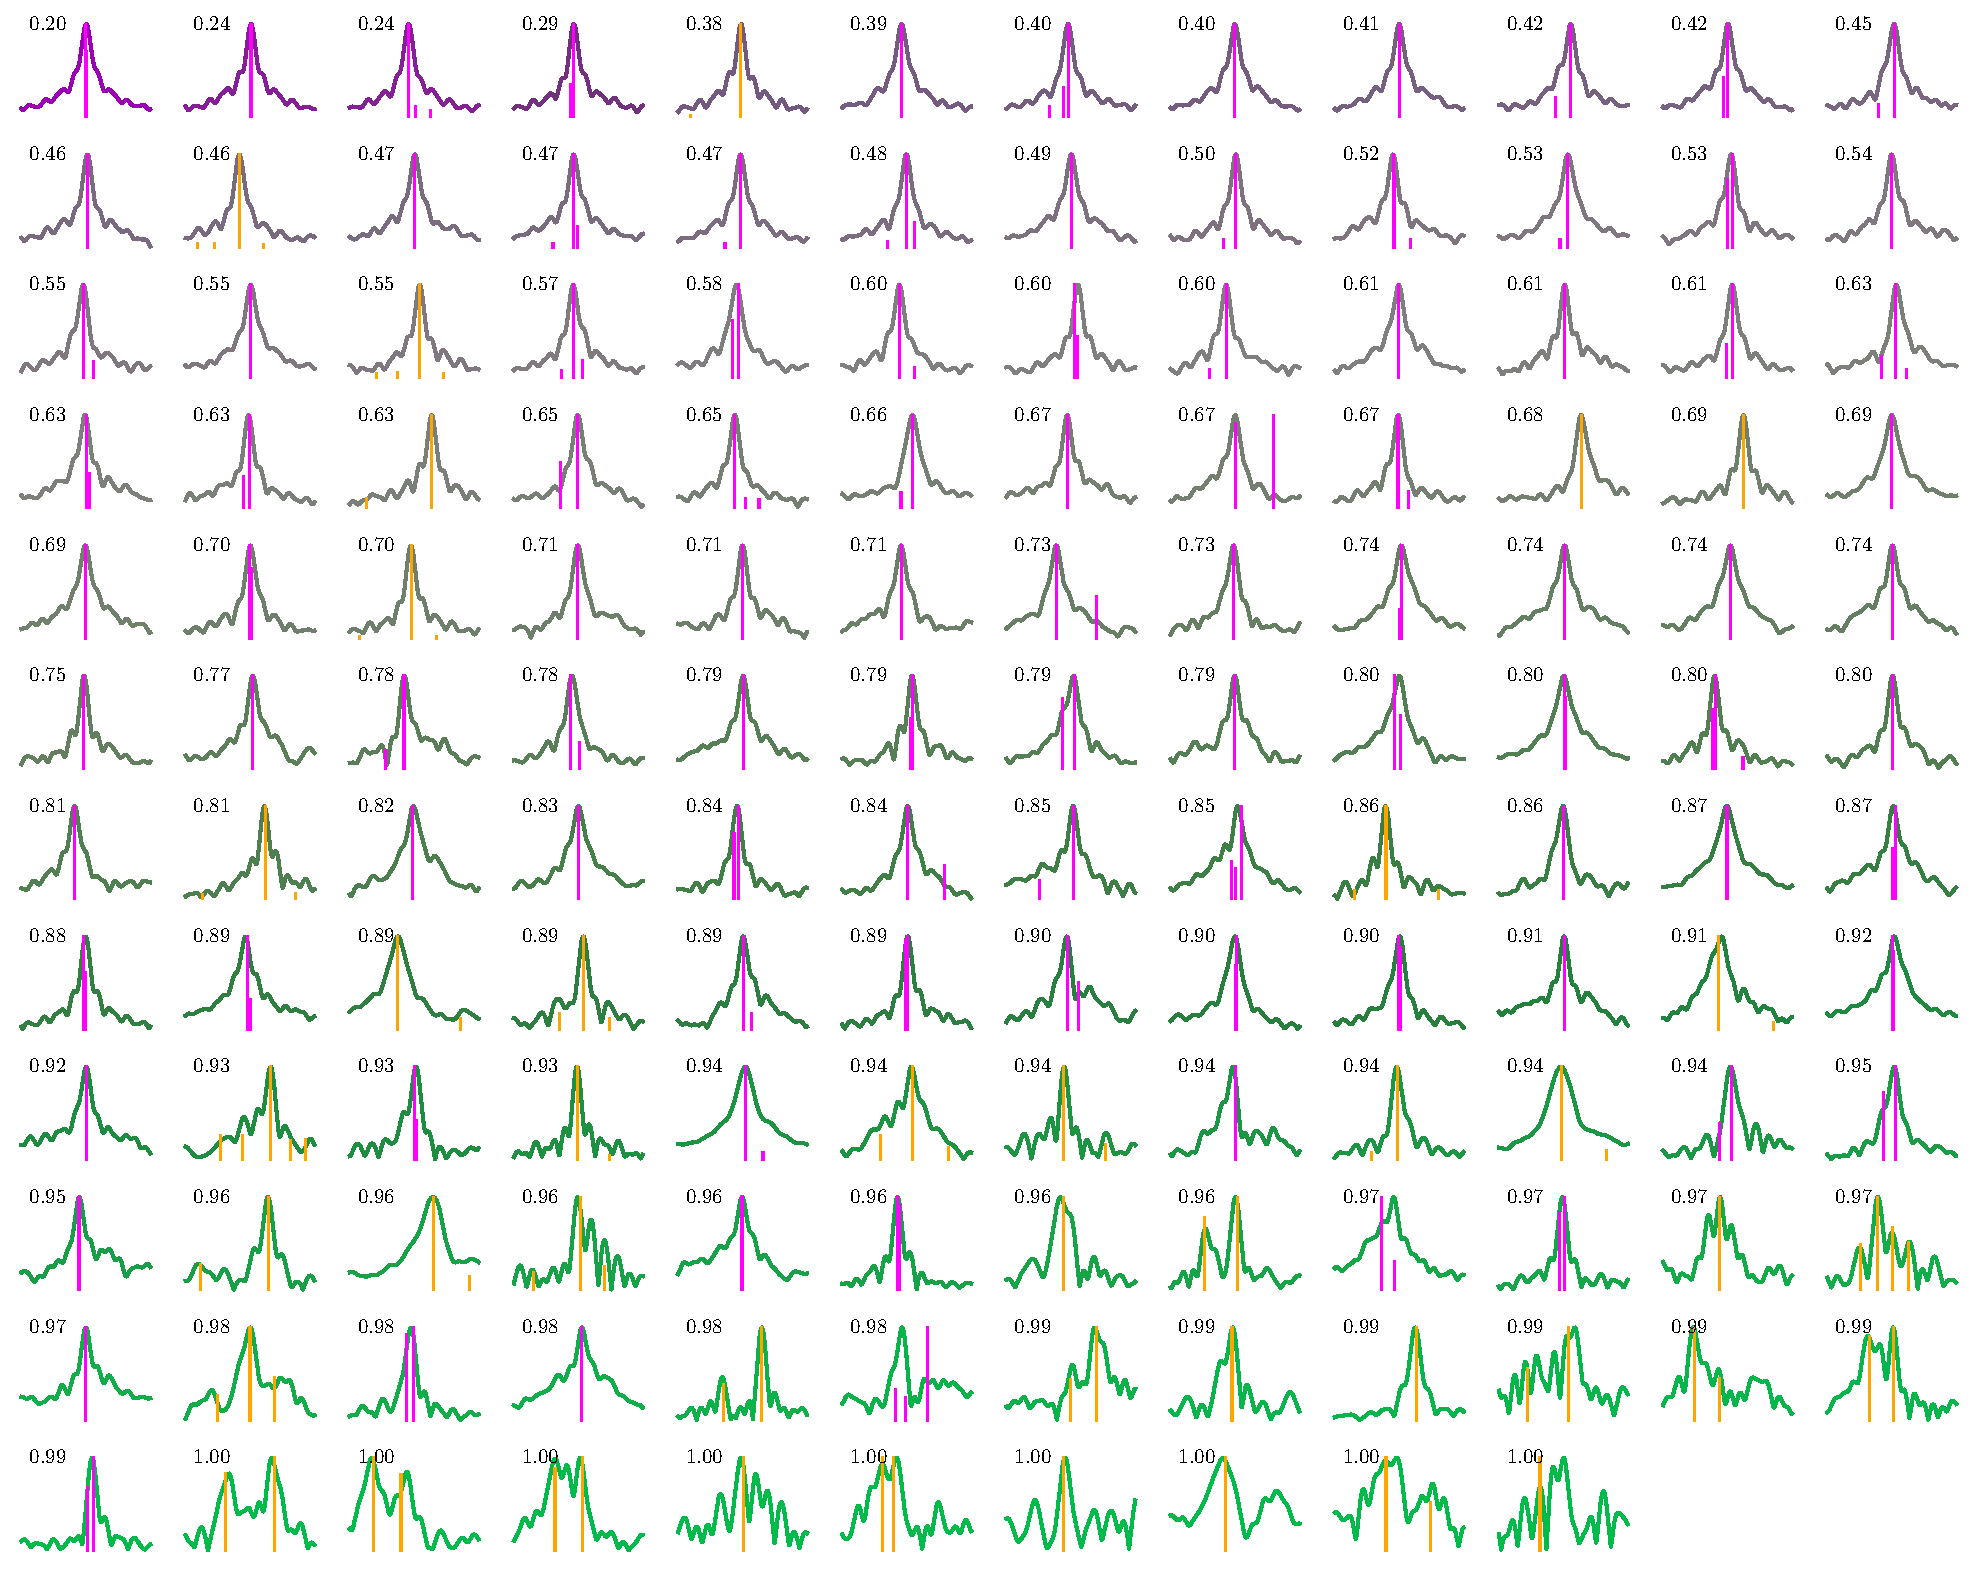
\includegraphics[width=\linewidth]{faraday-images/both_spectra_lr.pdf}
    % \includegraphics[width=0.7\linewidth]{faraday-images/jack_spectra.pdf}
    \caption{The 142 observed FDFs ordered by LR-estimated probability of being Faraday complex. Livingston-identified components are shown in orange while O'Sullivan-identified components are shown in magenta. Simpler FDFs are shown in purple while more complex FDFs are shown in green, and the numbers overlaid indicate the XGB estimate. A lower number indicates a lower probability that the corresponding source is complex, i.e. lower numbers correspond to simpler spectra.}
    \label{fig:all-observed-fdfs-lr}
  \end{figure*}

  \begin{figure*}
    \centering
    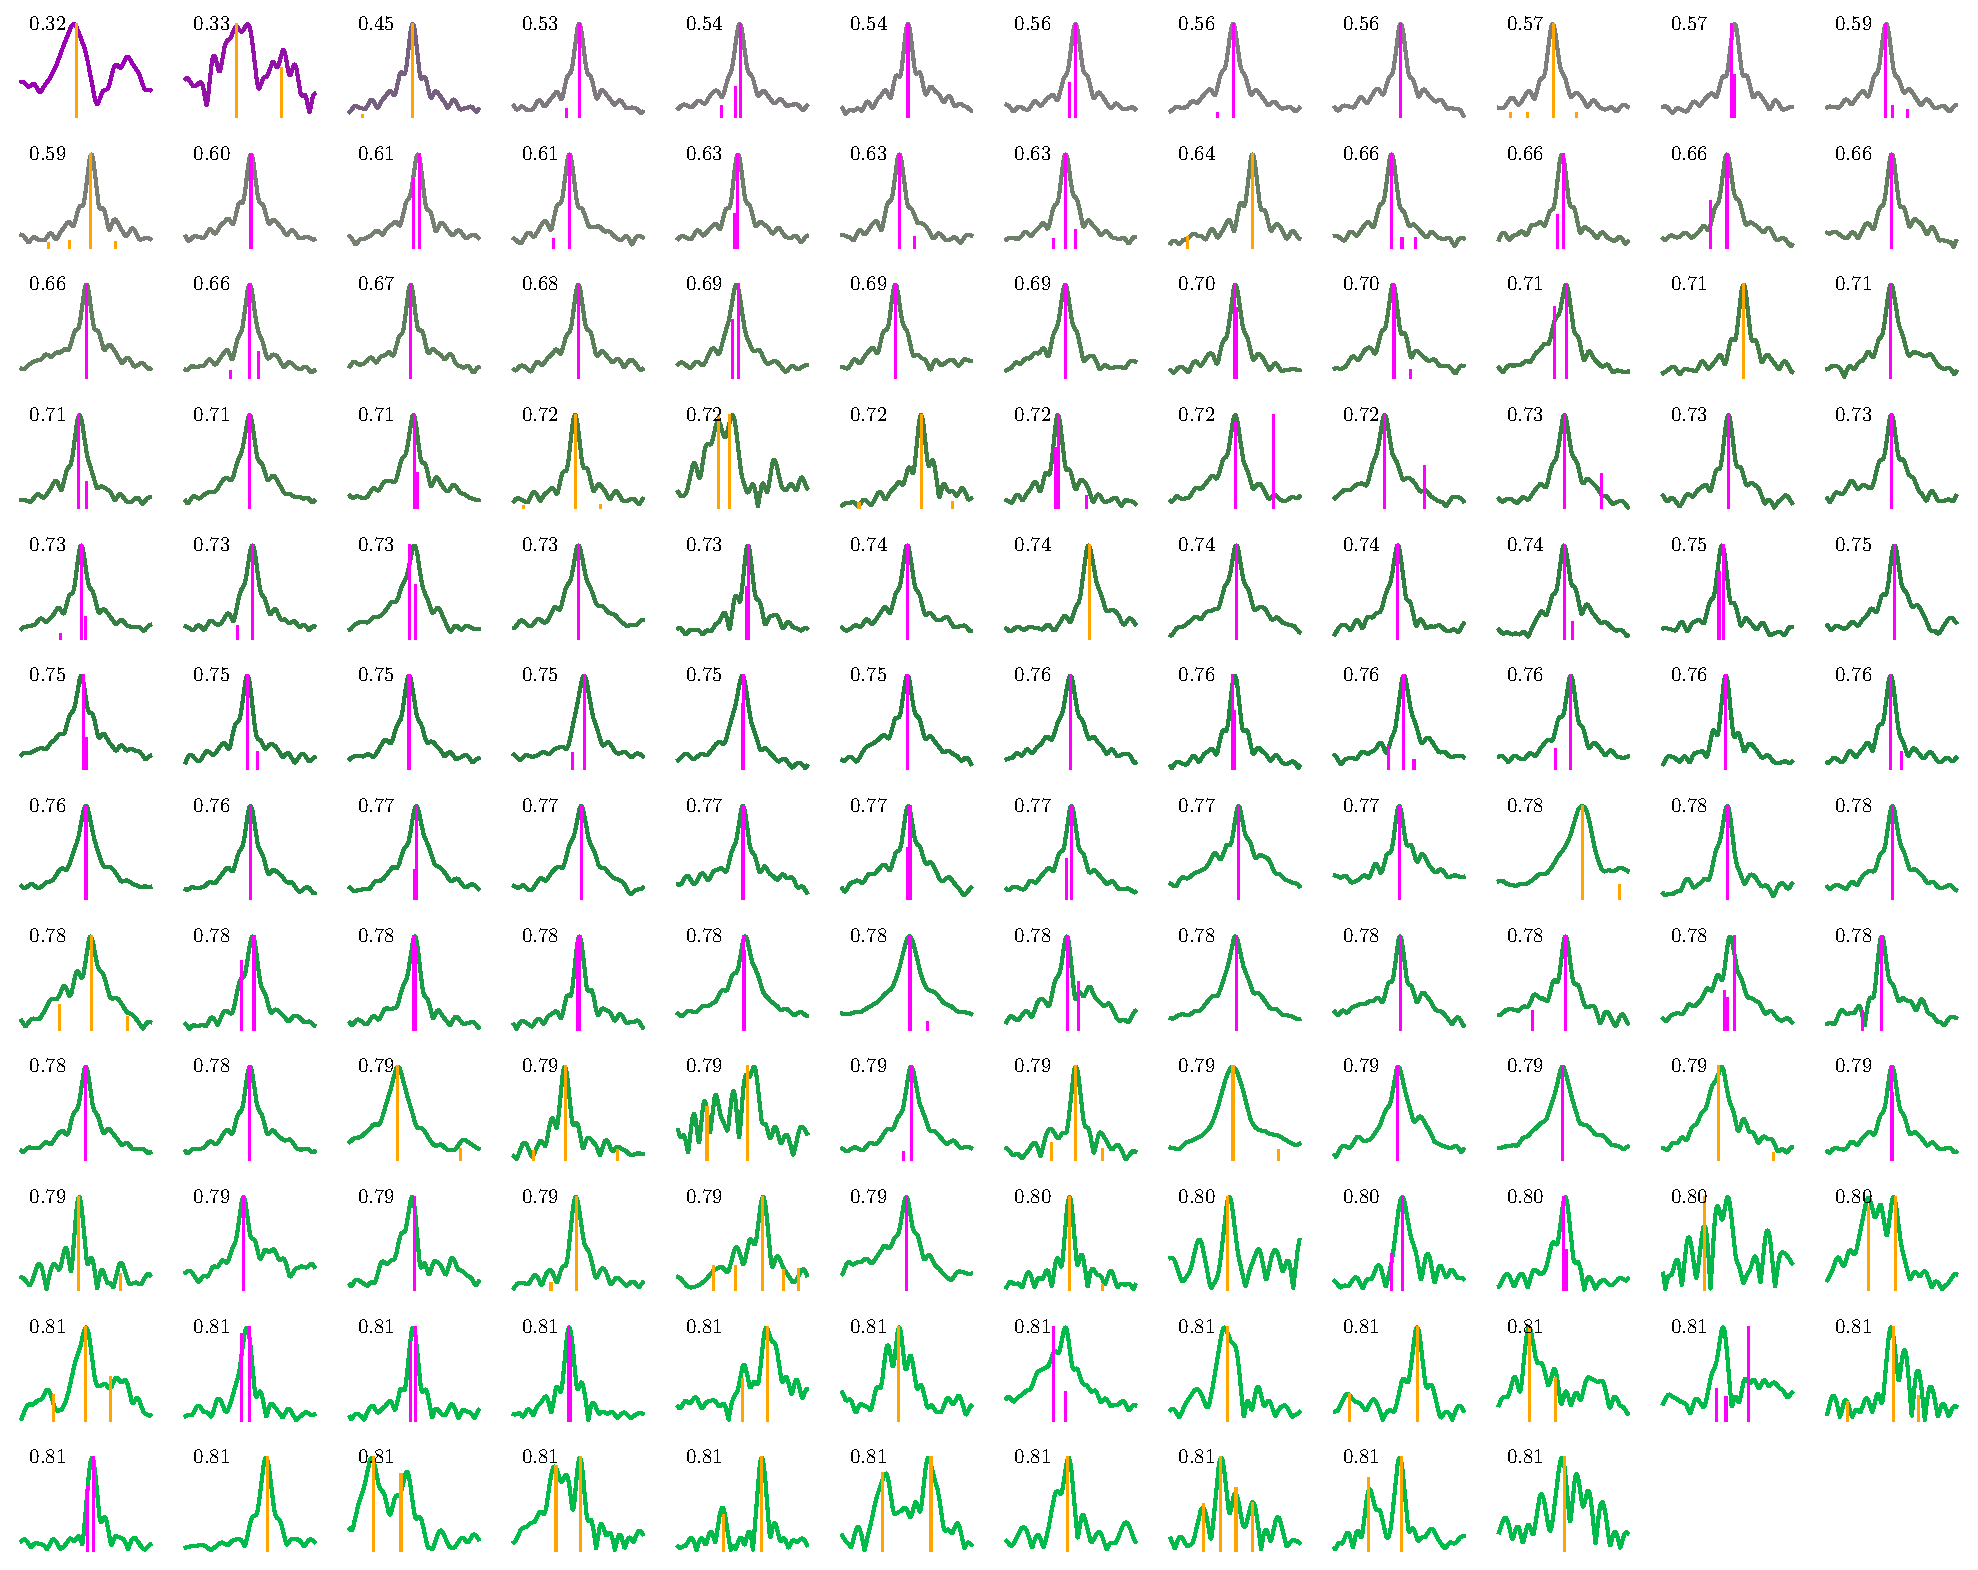
\includegraphics[width=\linewidth]{faraday-images/both_spectra_xgb.pdf}
    % \includegraphics[width=0.7\linewidth]{faraday-images/jack_spectra.pdf}
    \caption{The 142 observed FDFs ordered by XGB-estimated probability of being Faraday complex. Livingston-identified components are shown in orange while O'Sullivan-identified components are shown in magenta. Simpler FDFs are shown in purple while more complex FDFs are shown in green, and the numbers overlaid indicate the XGB estimate. A lower number indicates a lower probability that the corresponding source is complex, i.e. lower numbers correspond to simpler spectra.}
    \label{fig:all-observed-fdfs-xgb}
  \end{figure*}

\section{Simulating observed FDFs}
\label{sec:faraday-simulating}

  We simulated FDFs by approximating them by arrays of complex numbers. An FDF $F$ is approximated on the domain $[-\phi_{\max}, \phi_{\max}]$ by a vector $\vec F \in \mathbb R^d$:
    \begin{equation}
      \label{eq:faraday-vec-f}
      \vec F_j = \sum_{k = 0}^1 A_k \delta(-\phi_{\max} + j \delta \phi - \phi_k)
    \end{equation}
    where $\delta\phi = (\phi_{\max} - \phi_{\min}) / d$ and $d$ is the number of Faraday depth samples in the FDF.
    $\vec F$ is sampled by uniformly sampling its parameters:
    \begin{align}
      \label{eq:faraday-model-distributions}
      % p(\phi_0, \phi_1, A_0, A_1) = \frac{1}{(\phi_{\max} - \phi_{\min})^2} \begin{cases}
      %   1 & \phi_{0,1} \in [\phi_{\min} \phi_{\max}],\\
      %     & A_{0, 1} \in [0, 1];\\
      %   0 & \mathrm{otherwise}.
      % \end{cases}
      % p(\phi_k) &= \frac{1}{\phi_{\max} - \phi_{\min}} \begin{cases}
      %   1 & \phi_k \in [\phi_{\min} \phi_{\max}],\\
      %   0 & \mathrm{otherwise};
      % \end{cases}\\
      % p(A_k) &= \begin{cases}
      %   1 & \phi_k \in [0, 1],\\
      %   0 & \mathrm{otherwise};
      % \end{cases}
      \phi_k &\in [\phi_{\min}, \phi_{\min} + \delta\phi, \dots, \phi_{\max}]\\
      A_k &\sim \mathcal U(0, 1).
    \end{align}
    We then generate a vector polarisation spectrum $\vec P \in \mathbb R^m$ from $\vec F$ using a \autoref{eq:faraday-discrete-f-to-p}:
    \begin{equation}
      \label{eq:faraday-discrete-f-to-p}
      \vec P_\ell = \sum_{j = 0}^{j} F_j e^{2i(\phi_{\min} + j\delta_\phi)\lambda^2_\ell}\ \mathrm{d}\phi.
    \end{equation}
    $\lambda^2_\ell$ is the discretised value of $\lambda^2$ at the $\ell$th index of $\vec P$. This requires a set of $\lambda^2$ values, which depends on the dataset being simulated. These values can be treated as the channel wavelengths at which the polarisation spectrum was observed. We then add Gaussian noise with variance $\sigma^2$ to each element of $\vec P$ to obtain a discretised noisy observation $\hat{\vec{P}}$. Finally, we perform RM synthesis using the Canadian Initiative for Radio Astronomy Data Analysis \texttt{RM} package\footnote{\url{https://github.com/CIRADA-Tools/RM}}, which is a \texttt{Python} module that implements a discrete version of RM synthesis:
    \begin{equation}
      \label{eq:faraday-discrete-rm-synthesis}
      \hat{\vec{F}}_j = m^{-1} \sum_{\ell = 1}^m \vec{\hat P}_\ell e^{-2i(\phi_{\min} + j\delta_\phi)\lambda^2_\ell}.
    \end{equation}

\unappendix

  % If we were to run our classifiers at scale on the upcoming POSSUM survey, how would the limitations presented in \autoref{sec:faraday-results-simulated} affect derived statistics of Faraday complexity? 

  % \begin{itemize}
  %   \item Mention Brown cuts. What are the implications for POSSUM if we were to use our classifier? How does this affect what we can detect and can't?
  % \end{itemize}

  % \begin{itemize}
  %   \item (10) is a good example of noise being important but we can't explicitly factor it in yet - this is two peaks that are very different scales
  %   \item (27) is funky, we get a smooth-looking FDF but it's not obviously two peaks. see also (47)
  %   \item (38) has $\phi_s$ outside of the range! but it still looks good
  % \end{itemize}
%!tex engine=xelatex
%!tex root=./thesis.tex
\chapter{Conclusion}
\label{cha:conc}

% This chapter needs to
% \begin{itemize}
%     \item summarise the thesis
%     \item draw together works
%     \item link each chapter to theory and methodology
%     \item evaluate the contribution of this work to the field
%     \item discuss future work
% \end{itemize}

The future of radio astronomy is immensely exciting, with upcoming radio surveys like EMU and POSSUM sure to revolutionise our understanding of the violent Universe occupied by radio active galactic nuclei. In this thesis we have explored methods for identifying extragalactic radio sources in these future wide-area radio surveys.

\autoref{cha:cross-id} developed a new approach to cross-identifying radio components with their infrared host galaxies and applied this method to the CDFS and ELAIS-S1 ATLAS survey, a pilot survey for the upcoming ASKAP key survey EMU. This was the first ever application of machine learning to radio cross-identification. In the process, we demonstrated that our methods worked on ELAIS-S1 with similar performance to how they worked on CDFS, despite these being different parts of the sky. We also evaluated simple nearest-neighbour cross-identification on the ATLAS fields, showing better performance than either machine learning or Radio Galaxy Zoo volunteers on this dataset, which we suggest is because of how most objects in ATLAS are very compact. Our machine learning methods performed similarly whether they were trained on expert-provided or citizen science-provided labelled datasets, clearly demonstrating the benefit of citizen science labels to radio astroinformatics even if they may be less accurate than labels provided by experts. We showed that the algorithm we had developed could in principle perform much better than nearest-neighbours if only its binary accuracy could be raised, perhaps with a more complex or better-trained classifier. Finally, we concluded that ATLAS was an insufficiently complex dataset to train machine learning algorithms for future radio surveys: more complex and larger training sets would be necessary.

To further investigate our classification-based cross-identification algorithm we \linebreak needed a more complex dataset, and in \autoref{cha:rlfs} we turned to FIRST, a legacy survey containing around 900~000 radio components. Of these, 250~000 or so were not compact, compared to the vast majority of ATLAS. We increased the complexity of our machine learning model and trained it on this dataset along with 75~000 Radio Galaxy Zoo labels, far more than we had available for ATLAS. The resulting classifier could then be used to cross-identify every extended object in FIRST. Using the fact that any two radio components in the same radio source should also have the same host galaxy, we identified not only the host galaxies of our radio components but also their association to other radio components. This allowed us to produce a catalogue of over 150~000 extended radio sources, the largest existing catalogue of extended radio sources at the time of writing. Such a large catalogue enabled us to estimate a RLF for extended radio sources, the first time a RLF has been produced for just extended sources. We could also subdivide this RLF into a fractional RLF, and we were able to produce RLFs divided by the mid-infrared colour of the host galaxy, their physical extent, and their redshift. Extended radio sources ought to be the sources which contribute the most mechanical energy to their surrounding IGM, and with an RLF dedicated solely to extended sources we were able to estimate this energy contribution as $1.3 \times 10^{30}$ and $1.2 \times 10^{32}$~W~Mpc$^{-3}$. Perhaps most importantly, we showed our method works and used it to obtain a physically meaningful result. Our method can easily be extended to new surveys, as long as training data exist.

In \autoref{cha:faraday} we developed an interpretable Faraday complexity classifier. We constructed features that were easy to understand by measuring the distance of observations from a simple model of Faraday simple sources. Our resulting features could be calculated from both simulated and real observations. We demonstrated the effectiveness of our method on both simulated and real data and showed that on simulated data our simple methods matched the state-of-the-art CNN classifier despite having far less parameters. This was the first application of machine learning to real spectropolarimetric data. This method will be applicable to future surveys like POSSUM.

% \section{What we need to move forward}
% \label{sec:moving-forward}
    
%     What does radio astronomy need to be able to press ahead with astroinformatics? From my work what do we need to do to set ourselves up for a solid future field?

    % \begin{itemize}
    %     \item better training data
    %     \item more redshifts
    % \end{itemize}


\section{Future Work}
\label{sec:future}

    There are many ways that the research in this thesis can be extended in future. We will summarise some of these here.

    Our methods can be extended in a number of ways. These fall into two categories: further applications and extensions to the algorithms. An obvious target for future work is to apply our cross-identification algorithm to new and upcoming surveys like LoTSS and EMU. These promise a tremendous amount of data with new discoveries certain to be lying in wait within, and cross-identifying the radio emission with its corresponding infrared or optical host galaxy will be vital for uncovering those secrets. Similarly we would like to apply our Faraday complexity classifier to future spectropolarimetric surveys like POSSUM. Our methodology can also be improved. Better models almost certainly exist than the CNN we applied to BXID. As we demonstrated in \autoref{cha:faraday}, a well thought-out model and features may best a complex model like the CNN. How would our cross-identification approach worked if, say, we applied it to hand-selected features such as those chosen by \citet{proctor06}? Would a search over more CNN architectures, like that described by \citet{lukic_morphological_2019}, result in better classifiers and hence better cross-identifications? Perhaps we could even improve performance by pre-training on some unlabelled but larger dataset? A less obvious improvement to our BXID approach would be to change how the classification scores are aggregated. Currently this is a weighted maximisation over candidate host galaxies, but other methods are possible. The weights could be something other than a Gaussian function of distance, from other functions of distance to an entire separate classification model. Maybe we could aggregate the scores in bulk, using some kind of algorithm that assigns radio-host relationships based on not just the radio source itself but also on the other radio sources around it and how they have been paired to their own host galaxies.

    The way that our labels were generated for BXID could be improved. Our algorithms in \autoref{cha:cross-id} and \autoref{cha:rlfs} were trained on labels generated by Radio Galaxy Zoo. These labels were aggregated from multiple different labellers (usually 20) by majority vote, with the most common label for any give n radio object being assigned as the true label in Radio Galaxy Zoo. This is not the only possible aggregation strategy, though. We employed the Dawid-Skene method \citep{dawid79em} ourselves in \autoref{sec:rlfs-manual-validation} to help assess the performance of our cross-identification algorithm, and this model for example may also be applied to Radio Galaxy Zoo. There are in fact aggregation strategies that work in tandem with a machine learning model to get better labels, such as \citet{raykar_learning_2010}. These methods simultaneously take into account the labels and the labellers, and can accommodate for different levels of ability in the labellers, or different levels of difficulty in the examples being labelled.

    Our RLFs could be improved. The RLF calculations in \autoref{cha:rlfs} are severely limited by the availability of redshifts. We limit our analyses to host galaxies that do have available spectroscopic redshifts in SDSS, but we could also employ the less-reliable but considerably more prolific photometric redshifts. These are derived from regression models rather than direct observations of redshifted spectral lines, and so can be produced from photometric surveys without dedicated spectroscopy. However, without methods to handle the uncertainty introduced by photometric redshifts, the resulting RLFs would be unreliable. Developing ways to not only decrease the uncertainty in photometric redshifts but also to understand and incorporate the uncertainty into downstream calculations like those of the RLFs will allow these photometric redshifts to be used and tremendously increase sample sizes. This will be very important for surveys like EMU, which are both deep and wide with low redshift availability.

    The RGZ-Ex dataset (\autoref{cha:rlfs}) also lets us pose many other interesting science questions. We demonstrated in \autoref{sec:rlfs-giants} that rare galaxy classes can be identified from within this dataset, including examples that have never before been identified in the literature. Our dataset may be augmented with other features and used to identify unusual objects in a similar way. Besides this, our fractional RLFs could also be extended with any number of galaxy properties. One particularly interesting property could be morphology, as other algorithms in radio astroinformatics are developed which can automatically identify morphologies \citep[e.g.][]{wu19claran}: such a classifier could be used to segment RGZ-Ex and a fractional morphological RLF could be obtained. Of course, there are other properties that are more easily extracted, such as optical lines and colours which could be taken from SDSS using our SDSS cross-identifications.

     While creating features for FDFs in \autoref{cha:faraday} we demonstrated that W2 distance was a sensible distance measure between FDFs. This is useful for more than just feature construction, as it implies a geometry on the space of FDFs. This distance could be used to help gain insight on the behaviours of future algorithms that work on FDFs. A particularly exciting idea is to improve QU fitting by modifying the distance function to match ours. Our features could also be used to develop other methods for FDF analysis, like outlier detection or data visualisation.

     Further research is needed to close the domain gap for FDFs. This is an interesting case study as it is such a simple case, where we know essentially all the physics behind the observations and the observations are one-dimensional. Even this is not enough, and whether through unmodelled physics (e.g. more than two screens, depolarisation) or unmodelled observational properties (e.g. radio frequency interference) simulation and observation do not fully line up. This is critical if we want to train machine learning algorithms on simulations in the future, and we very much want to do this to augment our limited observational training data. Similarly the domain gap must be reduced for radio continuum imagery. Our results in \autoref{cha:cross-id} show that pilot surveys like ATLAS may not contain enough complex sources to train machine learning models, and while larger surveys like FIRST exist, transferring models from a survey undertaken with one set of observing parameters (telescope, frequency, depth, resolution...) is both non-trivial and as-yet relatively unexplored.

\section{Implications for radio citizen science}
\label{sec:implications-citizen-science}

    Our results in \autoref{cha:cross-id} demonstrated that machine learning methods trained on citizen science labels perform comparably to those trained on expert labels, even when those labels are lower quality than expert labels. We applied this insight in \autoref{cha:rlfs} to obtain scientific results, using machine learning to extrapolate the labels to a larger dataset. While Radio Galaxy Zoo alone was not enough to fully label FIRST, Radio Galaxy Zoo working in tandem with machine learning was. This is a pattern that may hold true for future surveys and applications, too. Future astronomical research at-scale may leverage the idea of people working with machine learning, sometimes called \defn{human-in-the-loop} \citep[e.g.][]{holzinger_interactive_2016} learning, to pore through data-at-scale.

\section{Implications for wide-area radio surveys}
\label{sec:implications-wide-area-radio-surveys}

    As we move toward larger and larger datasets, an important question is how applicable our models will be across the sky. Our results in \autoref{cha:cross-id} showed that we can expect some generalisation, as our model trained on one patch of sky was applicable to another without a great loss of performance. Similarly, our classifier trained on part of FIRST seemed to work well on the rest of the dataset. This is promising as it implies that limited area surveys may help develop training sets that generalise to the whole sky, potentially making the process of generating training sets considerably cheaper.

    Between \autoref{cha:cross-id} and \autoref{cha:rlfs} we demonstrated that a large set of good quality, complex data is required for training good astroinformatics algorithms. Pilot datasets like ATLAS will not work by themselves: the sources they contain are too simple and their complex sources are too few. A sensible question to ask is, could we simulate data for training purposes? We trained our classifier in \autoref{cha:faraday} on simulated data and found that it was difficult to bridge the domain gap between simulation and observation, even in a well-understood, one-dimensional case---let alone the complex three-dimensional projected morphologies we observe in imagery. Getting across this domain gap will be difficult and will necessarily be a major topic of research in the astroinformatics field in the near future.

    Tying observations, simulations, and models together are the representation of the data: features. Our results in \autoref{cha:faraday} show that judicious choice of features can outperform even complex and powerful models. This is good for two reasons. The first reason is that these features may be more easily interpreted. The meaning of the features may be understood to be representative of some physical property, or at least the relationship between physical reality and predictions may be more easily found. The second reason is that features may be selected which can generalise well to datasets beyond just the training set. In other words, features that are less overfit to the training set. This is of particular concern when developing predictive models on simulated training data, as features being less suited for real data than for simulations is one aspect that may contribute to the domain gap. Choosing good features in astronomy may be more important than in many other fields for which machine learning is applied, as while in most fields it is possible to conduct experiments, in astronomy we only have one Universe to look at. We need to make the best use we can of the limited radio sky.

    % - domain gap for training on simulated data for FDFs
    % - domain gap for simulated radio continuum data to augment surveys like ATLAS
    % - apply our cross-identification and Faraday complexity methods to EMU and POSSUM, as well as surveys like LoTSS and GLEAM-X
    % - improve our aggregation method for bxid
    % - generate alternative fractional RLFs, e.g. by ML-derived morphology
    % - incorporate photometric redshifts into calculations from rlf
    % - investigate the link between extended sources and their local environments
    % - apply other crowd aggregation strategies to RGZ
    % - use our insights into FDFs to do other interesting things, like outlier detection, data visualisation, or some new way of qu fitting


%%%%%%%%%%%%%%%%%%%%%%%%%%%%%%%%%%%%%%%%%%%%%%%%%%%%%%%%%%%%%%%%%%%%%%
% Here begins the end matter

%%% \appendix

\backmatter

\bibliographystyle{anuthesis}
\bibliography{thesis}

\printindex

\end{document}

